\documentclass[11pt]{article}

% ---------------- Packages ----------------
\usepackage[a4paper,margin=1in]{geometry}
\usepackage{amsmath,amssymb,amsfonts}
\usepackage{mathtools}
\usepackage{bm}
\usepackage{booktabs}
\usepackage{array}
\usepackage{longtable}
\usepackage{tabularx}
\usepackage{enumitem}
\usepackage{graphicx}
\usepackage{caption}
\usepackage{subcaption}
\usepackage{float}
\usepackage{xcolor}
\usepackage[colorlinks=true,linkcolor=blue,citecolor=blue,urlcolor=blue]{hyperref}
\usepackage[activate={true,nocompatibility},final,tracking=true,kerning=true,spacing=true,factor=1100,stretch=10,shrink=10,expansion=false,protrusion=true]{microtype}
\usepackage{setspace}
\usepackage{titlesec}
\usepackage{fancyhdr}
\usepackage{footmisc}
\usepackage{parskip}
\usepackage{url}
\usepackage{xspace}
\usepackage{authblk}
\usepackage[numbers,sort&compress]{natbib}

\emergencystretch=3em
\graphicspath{{figures_v4/}{figures_osd462/}}
\setlist[itemize]{leftmargin=1.6em,itemsep=0.25em,topsep=0.35em}
\setlist[enumerate]{leftmargin=1.6em,itemsep=0.25em,topsep=0.35em}
\titleformat{\section}{\Large\bfseries}{\thesection}{0.8em}{}
\titleformat{\subsection}{\large\bfseries}{\thesubsection}{0.8em}{}
\titleformat{\subsubsection}{\normalsize\bfseries\itshape}{\thesubsubsection}{0.6em}{}

\pagestyle{fancy}
\fancyhf{}
\fancyhead[L]{\small Mouse kidney spaceflight remodeling}
\fancyhead[R]{\small \thepage}
\renewcommand{\headrulewidth}{0.4pt}

\newcommand{\code}[1]{\texttt{#1}}
\newcommand{\pkg}[1]{\textsf{#1}}
\newcommand{\gene}[1]{\textit{#1}}
\newcommand{\RRRM}{RRRM-2\xspace}
\newcommand{\ISS}{ISS-T\xspace}
\newcommand{\LAR}{LAR\xspace}
\newcommand{\OSD}{OSDR\xspace}
\newcommand{\FDR}{FDR\xspace}

\title{\textbf{Cross-omic decoupling of transcriptomic remodeling and transporter activity in the mouse spaceflight kidney}\\[0.35em]
\large A recurrent matrix-high / DCT-low RNA context surrounds the established NCC/SPAK phosphorylation phenotype but does not propagate as a protein-abundance signature}
\author{Ibrahim Shahid}
\affil{Independent research draft for mentor feedback\\Authorship/collaboration structure pending}
\date{Draft v10, May 2026}

\begin{document}
\maketitle

% =====================================================================
\section*{Executive summary for mentor feedback}

\noindent\textbf{Purpose and scope of this draft.} This draft is framed as a \emph{cross-omic context-mapping study}. Its central finding --- and its organizing thesis --- is that spaceflight kidney remodeling is \emph{cross-omically decoupled}: the established distal-tubule NCC/SPAK transporter phenotype sits inside a recurrent kidney-wide RNA remodeling context, but that context does not propagate as a matching protein-abundance signature; it resolves most clearly at the regulatory-phosphorylation / activity layer. The definitive multi-omic, physiological, and morphological characterization of spaceflight-induced renal dysfunction, including the NCC dephosphorylation itself, has already been published as the Cosmic Kidney Disease study \citep{siew2024cosmic}; we do not re-discover it. Instead, the established phenotype is used as a fixed anchor, and the contribution is to ask what transcriptomic context surrounds it, at which omic layer it is expressed, and which stronger claims fail --- delineating honestly what transcriptomic pathway, regulator-activity, cell-type, and network analysis can and cannot add.

\vspace{0.6em}
\small
\begin{tabularx}{\textwidth}{>{\bfseries}p{0.22\textwidth}X}
\toprule
Question & Once the spaceflight DCT/NCC transporter phenotype is known, is it an isolated distal-tubule event, or does it sit inside a reproducible kidney-wide molecular context? If it sits inside a context, what is that context, at which omic layer is it expressed, and which stronger claims fail? \\
\midrule
Datasets & RRRM-2 / OSD-771 is the factorial bridge cohort (age $\times$ arm $\times$ flight). OSD-513 is an independent kidney flight recurrence cohort. OSD-253 is a metadata-aware strain/mechanism cohort (C57BL/6J vs C3H/HeJ). OSD-462 / RR-10 is the multi-omic anchor cohort (RNA-seq, proteomics, phosphoproteomics on the same animals); its kidney NCC dephosphorylation phenotype was first reported by \citet{siew2024cosmic}. Tabula Muris Senis kidney is an external aging reference. \\
\midrule
Relationship to prior work & The biological phenomenon --- spaceflight-associated renal transporter dephosphorylation and DCT remodeling --- is established by the Cosmic Kidney Disease study. This draft does not claim to discover it; it maps the reproducible RNA context around the established phenotype and the cross-omic boundaries that context obeys. \\
\midrule
Central finding & Spaceflight kidney remodeling is \emph{cross-omically decoupled}. A matrix-high / DCT-low RNA context recurs across RRRM-2 ISS-T, OSD-513, and OSD-462 RNA (pathway-vector cosine $0.87$, gate PASS). In OSD-462 it does \emph{not} translate to matrix or transporter protein abundance --- targeted concordance is null and matrix proteins move opposite their transcripts --- yet the WNK--SPAK/OSR1--NCC activating phosphorylation cluster is specifically and strongly suppressed, with total NCC protein flat. KSEA independently infers SPAK/OSR1 ($z=-6.31$) and WNK ($z=-4.12$) activity down. The recurrent transcriptomic context is real, but the measurable transporter lesion lives at the phosphorylation-activity layer, not at protein abundance. \\
\midrule
Cell-type bound & A marker-panel decomposition shows DCT identity \emph{and} transport fall while endothelial/stromal compartments rise recurrently across cohorts; per animal the endothelial score anti-correlates with NCC regulatory phosphorylation ($\rho=-0.76$, $p=0.0004$). The bulk DCT-low RNA signal therefore carries a genuine interstitial-expansion / composition component --- which is precisely why the phosphoproteome, not bulk RNA, is the reliable transporter readout. \\
\midrule
Evidence ladder & RNA-context recurrence $\rightarrow$ NCC/SPAK phospho-activity (measured, Tier 1) $\rightarrow$ DCT morphology (Cosmic Kidney Disease tNCC density $-48\%$, Tier 2 literature) $\rightarrow$ animal-matched physiology (Tier 3, absent here, named as future work). \\
\midrule
Boundaries & Animal-matched RNA$\leftrightarrow$NCC activity is concordant at group level but underpowered per-animal at $n=20$; an honest wrinkle (non-regulatory phosphosites also co-vary per-animal) is reported openly. Regulator-activity inference nominates no non-obvious upstream driver beyond expected injury programs; an endothelial/vascular TF axis is nominated only. LIONESS/node2vec network candidates do not translate to protein/phospho changes. RRRM-2 cannot support the original age-rewiring claim; OSD-253 shows TLR4/innate association, not requirement; the LAR arm attenuates rather than reverses. \\
\bottomrule
\end{tabularx}
\normalsize

\vspace{0.8em}
\noindent\textbf{Working claim structure.}
The sharp version of the central claim is one sentence: \emph{the established spaceflight DCT/NCC phenotype is embedded in a recurrent kidney-wide RNA remodeling context, but that context is cross-omically decoupled --- it recurs in transcriptomes, fails as a simple protein-abundance story, and converges most clearly on NCC/SPAK phosphorylation-activity suppression.} That is more interesting than ``matrix-high / DCT-low exists,'' because matrix and DCT biology are themselves expected; the contribution is the recurrent organization of that biology across spaceflight transcriptomes and its phospho-not-protein resolution in RR-10. The animal-matched and cell-type analyses bound the claim honestly: group-level RNA$\leftrightarrow$activity concordance is supported but per-animal prediction is underpowered, and the bulk DCT-low signal includes an interstitial-expansion component, so the regulatory-phosphosite layer is treated as the reliable transporter readout. Network methods and the original age-rewiring contrast are reported as negative boundaries, not protagonists.

\clearpage

\section*{Plain-language summary}

\noindent
Spaceflight harms the kidney. A recent landmark study, Cosmic Kidney Disease, showed using kidney tissue, urine, and blood from mice, rats, and astronauts that spaceflight chemically switches off a key salt-handling transporter in the distal kidney tubule, called NCC. This work does not try to re-discover that. Instead it asks a different question: once that ``switch-off'' is known, is it an isolated event, or does it sit inside a larger, repeating pattern of kidney change --- and if so, what does that pattern actually mean? Our main finding is what we call \emph{cross-omic decoupling}. Reading kidney genes (RNA), several \emph{separate} mouse spaceflight experiments show the same pattern: more matrix/scarring-type activity, less distal-tubule transport activity. But when, in the one cohort measured every way on the \emph{same kidneys}, we check whether that RNA pattern carries through to the proteins themselves, it does not --- protein amounts barely move, and some move the opposite way. The transporter ``switch-off'' shows up not as a change in how much protein there is, but as a change in a chemical modification that controls the protein's activity. A standard method confirms the upstream control kinases (WNK and SPAK) are turned down, as expected. We also looked at cell types: the RNA pattern partly reflects the distal tubule shrinking while scar-forming and blood-vessel cells expand --- which is exactly why the protein-modification layer, not bulk RNA, is the trustworthy readout of the transporter itself. We searched for a surprising hidden ``master switch'' behind all this and, honestly, did not find one beyond expected injury responses. The value of this paper is a careful, honest map of how a known transporter problem sits inside --- but is chemically decoupled from --- a wider kidney remodeling response.

\vspace{0.8em}

\begin{abstract}
\noindent
Prior multi-omic work --- the Cosmic Kidney Disease study --- established that spaceflight suppresses regulatory phosphorylation of the thiazide-sensitive Na--Cl cotransporter NCC and its activating kinases (SPAK/OSR1, WNK) in the distal convoluted tubule (DCT), defining a primary spaceflight tubulopathy \citep{siew2024cosmic}. What remains unclear is whether this transporter phenotype is an isolated distal-nephron event or part of a broader kidney-wide molecular context, and at which omic layer that context is expressed. We analyzed public mouse kidney spaceflight transcriptomes --- RRRM-2 (OSD-771), an age-by-arm-by-flight cohort, with the independent kidney flight cohorts OSD-513 and OSD-253 --- using a low-parameter contrast-vector framework, and anchored the resulting RNA context to matched RR-10 / OSD-462 RNA, TMT proteomic, and phosphoproteomic data acquired on the \emph{same animals}. We quantified the transporter phenotype as a kinase-activity endpoint by kinase-substrate enrichment analysis (KSEA), tested whether a phosphoproteomics-naive RNA score tracks measured NCC/SPAK phosphorylation animal-by-animal, decomposed the bulk RNA context into cell-type marker panels, and screened for non-obvious upstream regulators with the decoupler framework.

Across RRRM-2 ISS-T, OSD-513, and OSD-462 RNA, DCT/NCC-WNK transport suppression repeatedly co-occurred with ECM/stromal, adhesion, proteolytic, S1P/S1PR3, innate/macrophage, and stress-response programs, defining a recurrent matrix-high / DCT-low RNA context (OSD-462-vs-RRRM-2 pathway-vector cosine $0.87$, 95\% CI $0.65$--$0.90$; recurrence gate passed). In RR-10, however, this RNA context did \emph{not} translate into matrix or transporter protein-abundance change: pre-registered concordance was null for every targeted gene set, matrix proteins moved opposite their transcripts, and total NCC protein was unchanged ($+0.09$). Instead, the strongest molecular convergence was at the phosphorylation-activity layer: the WNK--SPAK/OSR1--NCC activating phosphosites were specifically suppressed (composite Ser65;Thr68 effect $-1.56$, $p=9.3\times10^{-7}$) while non-regulatory NCC sites were flat, and KSEA independently inferred SPAK/OSR1 ($z=-6.31$) and WNK ($z=-4.12$) activity loss. Spaceflight kidney remodeling is therefore \emph{cross-omically decoupled}: the recurrent transcriptomic context is real, but the measurable transporter lesion is post-translational rather than an abundance signature. A phosphoproteomics-naive RNA score and measured NCC regulatory phosphorylation were concordant at group level (flight lowers both; regulatory sites suppressed $\sim$4.3$\times$ more than non-regulatory sites) but the per-animal link was underpowered at $n=20$ (Spearman $\approx +0.33$, n.s.). A cell-type marker-panel decomposition showed DCT identity \emph{and} transport falling while endothelial and stromal compartments rose recurrently, with the per-animal endothelial score anti-correlating with NCC regulatory phosphorylation ($\rho=-0.76$, $p=0.0004$); the bulk DCT-low signal thus carries an interstitial-expansion component, reinforcing the phosphoproteome as the reliable transporter readout. Regulator-activity inference nominated no non-obvious upstream driver beyond expected injury programs, and LIONESS/node2vec network candidates did not translate to protein or phosphoprotein changes. These results position the known DCT/NCC spaceflight phenotype within a reproducible, cross-omically decoupled kidney remodeling context, and delineate honestly --- omic layer by omic layer --- what transcriptomic, regulator-activity, cell-type, and network analysis can and cannot establish.
\end{abstract}

\vspace{0.3em}
\noindent\textbf{Keywords:} spaceflight transcriptomics; mouse kidney; cross-omic decoupling; multi-omics; phenotype anchoring; OSD-771; RRRM-2; OSD-513; OSD-462; RR-10; cosmic kidney disease; proteomics; phosphoproteomics; distal convoluted tubule; NCC; SLC12A3; WNK-SPAK/OSR1; kinase-substrate enrichment; KSEA; cell-type decomposition; interstitial expansion; extracellular matrix; LIONESS; node2vec.

\clearpage
\tableofcontents
\clearpage

% =====================================================================
\section{Introduction}

\subsection{Spaceflight kidney biology is broader than kidney-stone risk}

Kidney risk has been part of human spaceflight medicine since early discussions of weightlessness-associated urolithiasis \citep{cockett1962astronautical}. Subsequent astronaut studies connected long-duration missions to altered calcium homeostasis, bone loss, and increased renal stone risk \citep{pietrzyk2007renal,smith2014men}. More recent space medicine has broadened this concern from stone formation alone to kidney remodeling, tubulopathy, solute handling, mitochondrial stress, vascular and interstitial changes, and multi-organ physiology \citep{siew2024cosmic,chouker2025impact,afshinnekoo2020fundamental}. Rodent spaceflight studies are central to this shift because kidney tissue can be collected directly and analyzed by histology, transcriptomics, and multi-omic profiling under controlled mission conditions \citep{daSilveira2020comprehensive,galazka2020rnaseq,finch2025strain}.

The biological question is not only whether spaceflight changes mean expression of individual genes. Kidney function depends on coordinated nephron-segment transport, immune activation, endothelial and interstitial remodeling, extracellular-matrix turnover, and stress-response programs. These processes can move together at module or pathway scale even when individual genes do not pass stringent differential-expression thresholds. Conversely, gene-level network metrics can look interesting without supporting a cohort-level biological program. The present study therefore treats network analysis as a multi-resolution problem: claims are strongest when pathway/module-scale direction, external recurrence, mechanism scoring, and exploratory gene prioritization point toward compatible biology.

\subsection{The Cosmic Kidney Disease study defines the phenotype this work maps}

The scientific framing of this manuscript is constrained by an important piece of prior work. \citet{siew2024cosmic} reported an integrated pan-omic, physiological, and morphological study of spaceflight-induced renal dysfunction --- termed Cosmic Kidney Disease --- using kidney tissue, urine, and serum from mice, rats, and astronauts. Among its central findings, that study reported that spaceflight induces renal transporter dephosphorylation, that two of the most strongly dephosphorylated proteins were the thiazide-sensitive Na--Cl cotransporter NCC (encoded by \gene{Slc12a3}) and related distal nephron transporters, and that the distal convoluted tubule undergoes structural remodeling with increased segment size but reduced overall tubule density. Critically, the mouse kidney phosphoproteomics in that work derives from the Rodent Research-10 (RR-10) mission, which is the same experiment deposited in the NASA Open Science Data Repository as OSD-462 and used as the multi-omic anchor cohort in the present analysis. The Cosmic Kidney Disease study therefore already establishes the biological phenomenon --- a primary spaceflight tubulopathy with NCC dephosphorylation --- at a level of evidence (multi-species, multi-omic, physiological, morphological) that the present transcriptomic analysis does not attempt to surpass.

This manuscript is consequently framed as a \emph{context-mapping} study rather than a discovery study. Because the Cosmic Kidney Disease study already establishes the transporter phenotype, the productive question is not whether the phenotype exists but what it means: once the DCT/NCC lesion is known, is it an isolated distal-tubule event, or does it sit inside a reproducible kidney-wide molecular context, and at which omic layer is that context expressed? That is not pure validation; it is interpretation and cross-omic triangulation around an established phenotype. Four questions follow. First, does a renal remodeling context compatible with the Cosmic Kidney Disease phenotype recur across mouse spaceflight RNA-seq cohorts that were not part of that study? Second, when that transcriptomic context is anchored against matched RR-10 protein and phosphoprotein data, does it propagate as protein abundance, or as regulatory-phosphorylation activity? Third, is the bulk RNA context a cell-autonomous transcriptional change or partly a shift in cell-type composition? Fourth, do regulator-activity inference and co-expression network methods nominate any non-obvious driver beyond expected injury biology? The answers, developed below, are: yes, the context recurs; it propagates as phosphorylation activity, not abundance --- the cross-omic decoupling that organizes this paper; it carries a genuine interstitial-expansion component; and no non-obvious driver emerges.

\subsection{Cross-omic decoupling, phenotype anchoring, and the evidence ladder}

The central finding and organizing thesis of this manuscript is \emph{cross-omic decoupling}. A recurrent transcriptomic remodeling context can exist --- and, as shown below, does --- without propagating to the protein-abundance layer in the way a naive reading of RNA would predict. In the spaceflight kidney, the matrix-high / DCT-low RNA context recurs across cohorts, but in the one cohort with matched proteomics and phosphoproteomics it does not become a matrix-protein or transporter-protein abundance change; the measurable transporter lesion instead resolves at the regulatory-phosphorylation / activity layer. This is more than the observation that ``matrix-high / DCT-low exists,'' which is biologically expected. It is a statement about how RNA, protein abundance, and phosphorylation behave in this specific setting, and it carries a concrete methodological warning: bulk-RNA recurrence should not be over-read as transporter-protein loss or matrix-protein deposition.

A persistent weakness of high-dimensional transcriptomic analysis is that its primary objects --- pathway scores, contrast vectors, network metrics --- are statistical constructs whose biological meaning is asserted rather than measured. A pathway score can move without any measured physiological consequence, and a moved score is not, by itself, a phenotype. This manuscript is therefore organized around a deliberate methodological choice: rather than letting a moved pathway score be the endpoint, the analysis is hung off an externally established, \emph{measured} molecular endpoint and asks whether the transcriptomic constructs co-vary with it. We refer to this as phenotype anchoring, by analogy with the anchoring of molecular signatures to imaging or histological endpoints in other organ systems; it is the method that lets cross-omic decoupling be stated as a graded result rather than an impression.

The anchor used here is the suppression of NCC/SPAK regulatory phosphorylation in the distal convoluted tubule. This endpoint is attractive for three reasons. It is measured directly by mass spectrometry rather than inferred from RNA; it is mechanistically specific, because the SPAK/OSR1-target phosphosites on NCC have defined activating roles in the WNK--SPAK/OSR1--NCC signaling chain \citep{ge2016wnk,castaneda2024dct}; and it is externally established as a genuine spaceflight phenotype by the Cosmic Kidney Disease study \citep{siew2024cosmic}, so anchoring to it does not depend on the present analysis being correct about the anchor itself.

The analysis is then structured as an explicit evidence ladder, in which each rung is a distinct and honestly graded level of evidence. The first rung is cross-cohort RNA-state recurrence: a matrix-high / DCT-low transcriptomic direction that recurs across independent mouse kidney spaceflight cohorts. The second rung, and the Tier-1 anchor, is the measured NCC/SPAK regulatory-phosphorylation activity in OSD-462 (RR-10), quantified here both as targeted phosphosite effects and, independently, by kinase-substrate enrichment analysis. The third rung is DCT morphology --- increased segment size with reduced tubule density --- which is a Tier-2 literature anchor taken directly from the Cosmic Kidney Disease study rather than measured here. The fourth rung is physiology --- urine and serum electrolyte handling, blood pressure --- which is not available in these datasets and is named explicitly as future work. Stating the ladder openly is itself part of the contribution: it makes precise which claims are measured, which are reproduced from literature, and which are aspirational.

The strongest test the available data permit is the link between the first and second rungs. Because OSD-462 / RR-10 ran kidney RNA-seq and phosphoproteomics on the \emph{same animals}, a per-animal DCT transport RNA score and a per-animal NCC regulatory-phosphorylation activity score can be matched by animal and compared directly. This animal-matched comparison is the closest this work comes to tying a transcriptomic construct to a measured phenotype, and its result --- group-level concordant, animal-level suggestive but underpowered --- is reported with that confidence label attached throughout.

One further caveat shapes the interpretation and is built into the analysis rather than left to the discussion. Bulk kidney RNA reflects not only transcriptional state within DCT cells but also nephron-segment composition, interstitial expansion, and immune infiltration. A ``DCT-low'' bulk signal could therefore be cell-autonomous transport suppression, a loss or dedifferentiation of DCT cells, or dilution of tubule transcripts by expanding non-tubule compartments. We address this directly with a cell-type marker-panel decomposition that separates DCT identity from the DCT transport program and tracks endothelial, stromal/fibroblast, and immune compartments. As shown below, the bulk DCT-low context carries a real interstitial-expansion component --- which does not overturn the cross-omic decoupling thesis but explains it, by showing why the phosphoproteome, normalized within itself, is the cleaner transporter readout than composition-confounded bulk RNA.

\subsection{RRRM-2 defines a clean factorial contrast with limited per-cell precision}

NASA RRRM-2 (OSD-771) is a rare mouse kidney RNA-seq cohort with Age, mission Arm, and Environment Group represented in the same study. Young and old female C57BL/6NTac mice were sampled across flight, habitat ground-control, vivarium, and basal contexts, with ISS terminal dissection (ISS-T) and live animal return (LAR) arms. This design naturally invites a factorial question: does spaceflight amplify, dampen, or redirect age-associated kidney transcriptional network patterns differently in ISS-T and LAR?

For an arm $a\in\{\mathrm{ISS\mbox{-}T},\mathrm{LAR}\}$, the within-arm control-aging vector and flight-aging vector can be written as
\begin{equation}
A^a_{GC}=\bar{X}_{\mathrm{Old},a,GC}-\bar{X}_{\mathrm{Young},a,GC},
\qquad
A^a_{FLT}=\bar{X}_{\mathrm{Old},a,FLT}-\bar{X}_{\mathrm{Young},a,FLT}.
\end{equation}
The original scientific aim was to compare $A^a_{FLT}$ with $A^a_{GC}$. Projection of $A^a_{FLT}$ onto $A^a_{GC}$ would quantify aging-like amplification or dampening, while the residual component would quantify redirection. This is a clean conceptual formulation. The statistical difficulty is that $A^a_{GC}$ itself is estimated from only ten mice within each arm (five young GC and five old GC). A noisy control-aging direction makes downstream claims about amplification or redirection unstable.

This is a property of the estimand. High-dimensional contrast-of-contrasts are harder than simple flight-versus-ground comparisons, especially for network features whose uncertainty is already larger than mean-expression uncertainty. The analysis below therefore separates the original age-rewiring hypothesis from the cross-cohort flight-remodeling question that RRRM-2 can answer when paired with independent OSDR cohorts.

\subsection{Role of WGCNA and sample-specific network analyses}

Weighted gene co-expression network analysis (WGCNA) is useful for identifying co-expression modules, module eigengenes, hub genes, module-trait associations, and module preservation \citep{langfelder2008wgcna,langfelder2011preservation}. It is a sensible structural annotation method for kidney transcriptomics. However, standard WGCNA does not naturally test the factorial interaction at the heart of this project. A module eigengene can show age association, flight association, or arm association, but the method summarizes a module by its dominant variance axis. A smaller-variance interaction pattern within a module can be blurred by the eigengene. WGCNA is therefore valuable here as a module-scale biological layer, not as the sole primary inferential engine for age-dependent network rewiring.

Sample-specific network methods such as LIONESS estimate how each sample contributes to a shared network structure \citep{kuijjer2019estimating}. Embedding methods such as node2vec provide low-dimensional summaries of graph neighborhoods \citep{grover2016node2vec}. These approaches are useful for asking whether a gene's local network context changes, in addition to whether its mean expression changes. Given the cohort size and multiple-testing burden, this manuscript uses LIONESS/node2vec as exploratory local-neighborhood prioritization after establishing the pathway/module-level recurring direction.

\subsection{A cross-cohort contrast strategy}

The strategy in this manuscript is to pair RRRM-2 with external OSDR cohorts at the level of comparable pathway contrasts. RRRM-2 supplies the factorial bridge: it defines ISS-T and LAR flight directions under a controlled design. OSD-513 supplies an independent flight-vector recurrence test. OSD-253 supplies mechanistic and metadata-aware context because it includes C57BL/6J and C3H/HeJ mice and because C3H/HeJ has defective TLR4 signaling, making it useful for constraining TLR4-dependent interpretations. OSD-253 is analyzed as a mechanism-context cohort because original and rerun ground-control definitions trade off light history and sequencing/read-length comparability, and rodent spaceflight transcriptomes are known to be sensitive to sample collection and preservation factors \citep{galazka2020rnaseq,preserve2016}. Finally, OSD-462 (RR-10) supplies the multi-omic anchor: it is the only cohort in this analysis with matched kidney RNA-seq, TMT proteomics, and phosphoproteomics, and it is the cohort whose NCC phenotype was characterized by the Cosmic Kidney Disease study \citep{siew2024cosmic}. It therefore allows the transcriptomic remodeling direction to be tested against protein and phosphoprotein evidence and against an externally established benchmark.

The resulting analysis is organized as a deliberate claim hierarchy. First, RRRM-2 is tested for the original age-rewiring claim. Second, RRRM-2 arm-specific flight vectors are tested against OSD-513. Third, the aligned direction is decomposed into a matrix-high / DCT-low tubulointerstitial state. Fourth, LAR is tested against three competing models: attenuation, true reversal, and mechanism switch. Fifth, OSD-253 is used to ask whether the state is TLR4-associated or TLR4-dependent. Sixth, WGCNA, LIONESS, and node2vec are used to annotate and prioritize genes within the pathway-level program. Seventh, the pre-registered OSD-462 multi-omic anchor tests whether the RNA direction reproduces and whether it corresponds to protein-abundance or phosphorylation-level evidence of transporter remodeling. Eighth, the measured phenotype is quantified as a regulator-activity endpoint by KSEA, and the transcriptomic DCT transport program is compared --- animal-by-animal within RR-10 --- against the measured NCC regulatory-phosphorylation activity, completing the phenotype-anchoring link. Every step records which claims it supports and, equally, which it does not.

% =====================================================================
\section{Methods}

\begin{figure}[H]
\centering
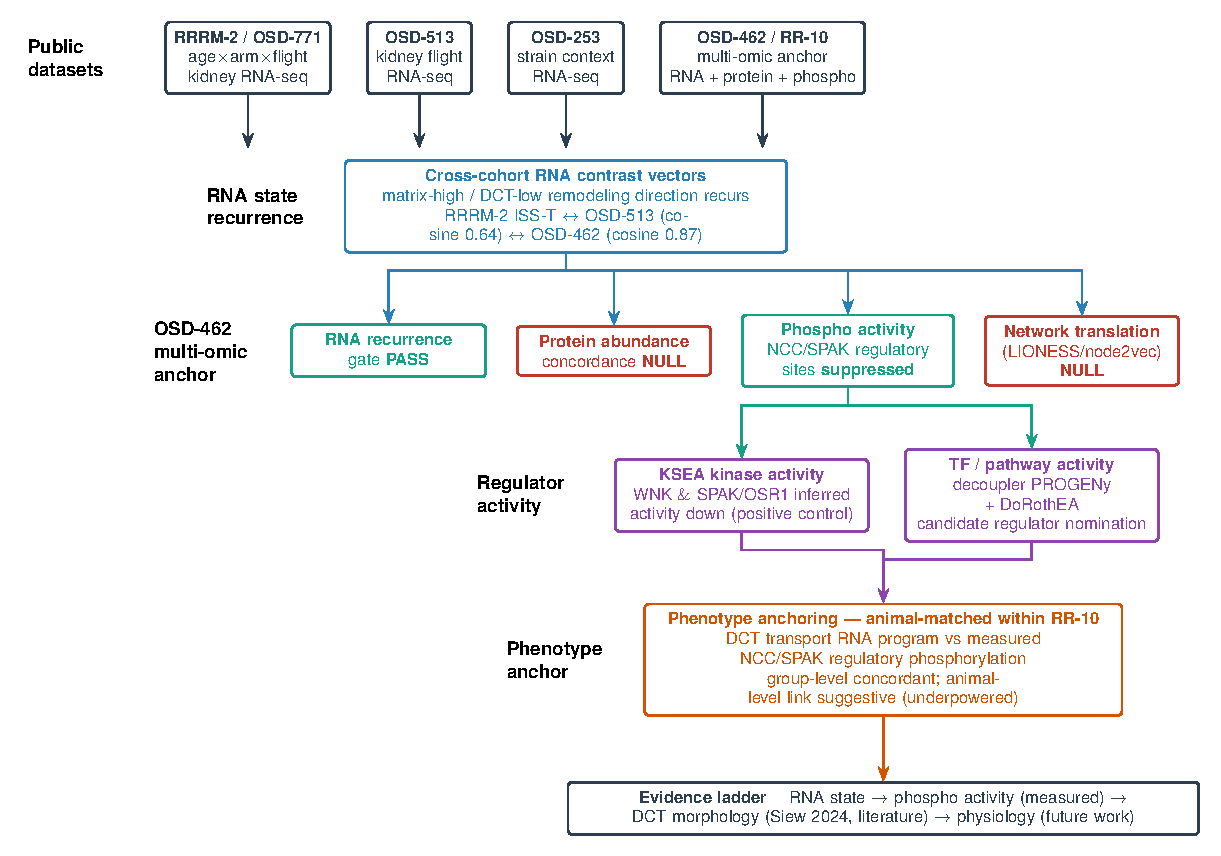
\includegraphics[width=\textwidth]{methodology_overview.pdf}
\caption{\textbf{Methodology overview --- the phenotype-anchored evidence ladder.} Four public mouse kidney spaceflight datasets feed a cross-cohort RNA-state contrast in which a matrix-high / DCT-low remodeling direction recurs (RRRM-2 ISS-T $\leftrightarrow$ OSD-513 $\leftrightarrow$ OSD-462). The OSD-462 / RR-10 cohort serves as the multi-omic anchor: the RNA recurrence gate passes, protein-abundance concordance is null, the WNK--SPAK/OSR1--NCC regulatory phosphosites are suppressed, and LIONESS/node2vec network translation is null. Regulator-activity inference (KSEA kinase activity as a positive control; decoupler PROGENy/DoRothEA for candidate TF/pathway nomination) and the animal-matched phenotype-anchoring comparison (DCT transport RNA program versus measured NCC/SPAK regulatory phosphorylation, within RR-10) sit on top of the anchor. The whole structure is read as an evidence ladder: RNA state $\rightarrow$ phospho activity (measured, Tier 1) $\rightarrow$ DCT morphology (literature, Tier 2) $\rightarrow$ physiology (Tier 3, future work).}
\label{fig:methodology}
\end{figure}

\subsection{Datasets and metadata handling}

\subsubsection{RRRM-2 / OSD-771}

RRRM-2 (OSD-771) was the discovery and factorial bridge cohort. The analysis used kidney RNA-seq from female C57BL/6NTac mice in a design crossing Age (Young and Old), mission Arm (ISS-T and LAR), and Environment Group (FLT, Habitat Ground Control, Vivarium Control, Basal), with $n=5$ biological replicates per Age $\times$ Arm $\times$ Environment cell. ISS-T and LAR were treated as distinct mission-arm/recovery-context strata rather than as a simple duration contrast. Primary flight contrasts used FLT and Habitat Ground Control samples. Vivarium and Basal samples were retained for preprocessing context and metadata completeness but were not pooled into the primary FLT-versus-GC vectors.

\subsubsection{OSD-513}

OSD-513 was used as the primary external recurrence cohort because it contains a powered mouse kidney flight comparison with $n=9$ FLT and $n=9$ Habitat Ground Control samples, plus additional context samples. It is not identical to RRRM-2 in sex, mission, strain substrain, or metadata, so it was not pooled with RRRM-2 at raw-expression level. Instead, the OSD-513 flight-minus-ground pathway vector was compared to RRRM-2 arm-specific flight vectors.

\subsubsection{OSD-253}

OSD-253 was used as a mechanistic and metadata-aware context cohort. It contains C57BL/6J and C3H/HeJ samples and therefore provides an opportunity to ask whether an ISS-T-aligned remodeling score is attenuated in a TLR4-impaired strain background. However, OSD-253 also has control-definition complexity. Original ground controls are closer to the original sequencing context but have light-history mismatch, whereas 2021 white-LED rerun controls improve the light comparison but introduce read-length/library comparability concerns. Therefore, both scenarios were run, and OSD-253 was not treated as a single clean validation endpoint.

\subsubsection{External kidney aging reference}

Tabula Muris Senis kidney data were used to construct an independent mouse kidney aging axis \citep{tabula2020}. Female kidney single-cell profiles were aggregated to donor-level pseudobulk expression, and the primary external aging vector was defined as 18-month minus 3-month donor expression. This reference is useful because it prevents the small RRRM-2 GC aging direction from being the only definition of kidney aging, but it differs from RRRM-2 in age range, platform, and cell capture.

\subsection{Expression preprocessing and residualized matrix}

All primary RRRM-2 analyses used the residualized expression matrix and matched sample metadata generated by the project preprocessing pipeline. Upstream preprocessing included expression filtering, variance-stabilizing transformation, cell-type deconvolution, and residualization against technical and cellular-composition covariates. The purpose of residualization was to reduce the chance that apparent network or pathway shifts were driven only by changes in estimated kidney cell-type proportions. The residualized matrix was used for pathway scoring, module projection, and sample-specific node summaries.

External OSDR cohorts were processed with study-specific expression resources. Because OSDR studies differ in mission design, sequencing details, strain, sex, and metadata structure, external cohorts were compared at the level of within-study contrasts rather than by pooled sample-level modeling.

\subsection{Feature resolutions}

Four feature resolutions were used.

\textbf{Pathway resolution.} Curated kidney-relevant gene sets were scored per sample by averaging residualized expression across genes represented in the feature universe. The main pathway panel included DCT/NCC-WNK transport, ECM remodeling, fibrosis, apoptosis, oxidative stress, inflammation, calcium handling, lipid metabolism, and broad ion transport. DCT/NCC-WNK was designated as the primary tubular-transport feature because it is more mechanistically coherent than broad ion transport.

\textbf{Module resolution.} WGCNA module eigengenes from the existing module run were used as module-level features. WGCNA modules were used to annotate coherent gene programs and to ask whether pathway-scale effects map onto unsupervised co-expression architecture.

\textbf{Gene resolution.} Gene-level expression features were retained for sensitivity and exploratory analyses. Gene-level analyses were never used to override module/pathway stability because they carry larger multiple-testing and interpretability burdens.

\textbf{LIONESS-node and node2vec resolution.} LIONESS sample-specific networks were built on a shared topology/backbone. Per-sample incident edge strengths were aggregated to gene-level node-strength features. Separately, condition-level graph embeddings were aligned by Procrustes transformation and used to compute local-neighborhood displacement. These quantities were used only for exploratory candidate prioritization.

\subsection{Within-RRRM age-vector stability and decomposition}

For each arm and feature resolution, a control-aging vector was computed as Old GC minus Young GC:
\begin{equation}
A^a_{GC}=\bar{X}_{\mathrm{Old},a,GC}-\bar{X}_{\mathrm{Young},a,GC}.
\end{equation}
Bootstrap resampling was stratified by Age, Arm, and Environment Group. Each bootstrap replicate rebuilt $A^a_{GC}$ and computed its cosine similarity to the full-sample vector. Module and pathway resolutions were treated as primary biological resolutions. Gene and LIONESS-node resolutions were treated as secondary.

If a primary control-aging direction was stable, the planned decomposition would compare the flight-aging vector
\begin{equation}
A^a_{FLT}=\bar{X}_{\mathrm{Old},a,FLT}-\bar{X}_{\mathrm{Young},a,FLT}
\end{equation}
to $A^a_{GC}$. The projection coefficient
\begin{equation}
\beta^a = \frac{A^a_{FLT}\cdot A^a_{GC}}{\lVert A^a_{GC}\rVert^2}
\end{equation}
would quantify alignment along the control-aging axis: $\beta>1$ suggests amplification, $0<\beta<1$ suggests dampening, $\beta<0$ suggests reversal, and a large orthogonal residual suggests redirection. In the production run, primary module/pathway stability did not pass consistently, so this decomposition is not promoted as a main biological claim.

\subsection{Cross-OSDR flight-vector recurrence}

The arm-specific RRRM-2 flight vector at pathway resolution was computed as age-pooled FLT minus GC within each arm:
\begin{equation}
F^{\mathrm{RRRM2},a}=\bar{X}_{\mathrm{FLT},a}-\bar{X}_{\mathrm{GC},a}.
\end{equation}
For an external study $s$, the corresponding flight vector was
\begin{equation}
F^s=\bar{X}^s_{\mathrm{FLT}}-\bar{X}^s_{\mathrm{GC}}.
\end{equation}
Vectors were compared using cosine similarity over shared pathway features. External uncertainty was estimated by bootstrap resampling within FLT and GC strata. A label-permutation sensitivity was also added for each external study/scenario by shuffling FLT/GC labels within the external cohort while holding the RRRM-2 arm-specific reference vector fixed. Directional permutation $p$ values report the fraction of shuffled external contrasts with cosine at least as positive as the observed value for positive alignments, or at least as negative for anti-alignments. OSD-513 was interpreted under a recurrence boundary. OSD-253 was interpreted under a context-sensitivity boundary because of metadata and control-scenario caveats.

\subsection{Recurrent remodeling-axis construction}

A recurrent ISS-T remodeling axis was constructed from pathways that were concordant between RRRM-2 ISS-T and OSD-513. Let $u_p$ be the unit-normalized RRRM-2 ISS-T effect for pathway $p$ and $v_p$ the unit-normalized OSD-513 effect. The raw pathway weight was the mean directional contribution from the two cohorts. The final axis was oriented so ECM/fibrosis activity was positive and DCT/NCC-WNK transport suppression was negative. Pathways with discordant signs were excluded from the primary axis. Broad ion transport was retained only as a sensitivity feature when its direction was mixed.

For each sample $i$, a scalar remodeling score was computed as
\begin{equation}
S_i = \sum_{p\in P_{\mathrm{axis}}} z(X_{ip})w_p,
\end{equation}
where $z(X_{ip})$ is the standardized pathway activity and $w_p$ is the unit-normalized recurrent-axis weight. Higher $S_i$ indicates a sample that is more similar to the recurrent ISS-T/OSD-513 remodeling direction.

\subsection{Mechanism scoring}

Mechanism signatures were defined in the versioned mechanism gene-set configuration file. Signatures included TLR4/innate immune signaling, TGF-beta/EMT/fibrosis, ECM organization, integrin/cell adhesion, S1P/S1PR3 signaling, MMP/ADAM proteolysis, DCT/NCC-WNK transport, broad tubular transport, oxidative stress/NRF2, macrophage/inflammatory context, and preservation/sample-stress response. Signatures were assigned roles as outcome anchors, candidate upstream mechanisms, or candidate context signatures.

To reduce circularity, axis-defining genes were dropped from mechanism signatures where possible before scoring. Coverage reports recorded requested genes, matched genes, scored genes, axis-overlap removals, and dropped genes. Mechanism scores were then tested against the scalar remodeling score by Spearman correlation within RRRM-2, OSD-513, and OSD-253. RRRM-2 and OSD-513 flight-minus-ground effects were also computed for mechanism scores.

\subsection{Tubulointerstitial state-space analysis}

The recurrent remodeling axis was also represented as a two-dimensional tubulointerstitial state space. This step was designed to make the biology legible without sign-flipping the DCT/NCC-WNK component. For each sample, mechanism scores were standardized within each study/scenario context. The matrix component was defined as
\begin{equation}
M_i=\frac{z(\mathrm{ECM}_i)+z(\mathrm{Integrin/adhesion}_i)+z(\mathrm{MMP/ADAM}_i)}{3}.
\end{equation}
The DCT transport component was defined in its native direction:
\begin{equation}
T_i=z(\mathrm{DCT/NCC\mbox{-}WNK}_i),
\end{equation}
where higher $T_i$ means stronger DCT/NCC-WNK transport signature. The plotted state space uses $M_i$ on the x-axis and $T_i$ on the y-axis. The matrix-high / DCT-low remodeling direction is therefore rightward and downward. A scalar state score was defined separately as
\begin{equation}
R_i=M_i-T_i.
\end{equation}
Higher $R_i$ means higher ECM/adhesion/proteolysis activity and lower DCT/NCC-WNK transport.

Two context components were computed in parallel: an immune-context component, defined as the mean of TLR4/innate and macrophage/inflammation z-scores, and a preservation-stress component, defined as the preservation/sample-stress z-score. FLT-minus-GC effects were computed for RRRM-2 ISS-T and LAR, age-pooled and age-stratified; OSD-513 FLT versus habitat ground control; and OSD-253 C57BL/6J and C3H/HeJ under both original-GC and white-LED rerun control definitions.

RRRM-2 state-space scores were joined to existing deconvolution outputs for DCT, fibroblast, immune, endothelial, proximal tubule, and TAL/LOH proportions. Spearman correlations tested whether $M_i$, $T_i$, immune context, preservation stress, or $R_i$ tracked estimated cell proportions. A targeted renal gene panel was extracted from the residualized RRRM-2 expression matrix for ECM/adhesion/proteolysis genes, TLR/innate/macrophage genes, DCT/NCC-WNK transport genes, and tubular/metabolic/network-priority genes observed in earlier analyses. This panel was used for biological visualization, not as an additional genome-wide discovery test.

\subsection{Live-return arm attenuation/divergence analysis}

The LAR anti-alignment raised a separate biological question: does live animal return simply attenuate the ISS-T remodeling response, move in the opposite direction, or switch into another program? We therefore defined three competing models before interpreting the data. Model A was attenuation or recovery-to-baseline, where the LAR FLT-minus-GC vector is near zero relative to ISS-T. Model B was true reversal, where the LAR vector is stably opposite to ISS-T and the LAR effect itself is non-zero. Model C was mechanism switch, where LAR is not simply the negative of ISS-T but instead loads onto other programs such as clock/DCT transcriptional state, S1P/vascular-interstitial signaling, preservation/cold-stress context, immune resolution, or persistent tubular transport disruption.

For each feature set $X$, arm-specific flight vectors were defined as
\begin{equation}
v_{\mathrm{ISS}}=\bar{X}_{\mathrm{ISS},FLT}-\bar{X}_{\mathrm{ISS},GC},
\qquad
v_{\mathrm{LAR}}=\bar{X}_{\mathrm{LAR},FLT}-\bar{X}_{\mathrm{LAR},GC}.
\end{equation}
Age-pooled effects were computed as the mean of young and old age-stratified FLT-minus-GC contrasts to keep age strata balanced. Reversal was quantified by
\begin{equation}
\cos(v_{\mathrm{LAR}},v_{\mathrm{ISS}})
\end{equation}
and by the projection coefficient
\begin{equation}
\beta_{\mathrm{LAR}\rightarrow \mathrm{ISS}}
=\frac{v_{\mathrm{LAR}}\cdot v_{\mathrm{ISS}}}{\lVert v_{\mathrm{ISS}}\rVert^2}.
\end{equation}
Negative cosine indicates an opposite direction; negative $\beta$ indicates movement opposite the ISS-T direction with magnitude interpretable on the ISS-T scale. Bootstrap confidence intervals resampled samples within Arm $\times$ Age $\times$ condition cells. Permutation sensitivities shuffled FLT/GC labels within Arm $\times$ Age strata. For state-space vector geometry, \code{matrix\_minus\_dct} was excluded from the feature vector because it is exactly \code{matrix\_component} minus \code{dct\_transport\_component}; it was retained only as a scalar readout in effect and interaction tables.

The reversal test was run at state-space, mechanism-score, WGCNA-module eigengene, all-gene residual-expression, and exploratory LIONESS/node2vec-summary levels. A feature set was labeled as a reversal candidate when the LAR/ISS-T cosine was negative with bootstrap CI excluding zero and $\beta_{\mathrm{LAR}\rightarrow \mathrm{ISS}}\leq -0.25$. A feature set was labeled attenuation when LAR magnitude was small relative to ISS-T and $|\beta|<0.25$. Intermediate negative cosines were labeled partial reversal or switch.

Component-level arm-by-flight interactions were computed for matrix component, DCT transport, immune context, preservation stress, matrix-minus-DCT, ECM organization, S1P/S1PR3, clock-gene scores, Rbm3/preservation scores, and related targeted panels. For each feature $f$, the interaction was
\begin{equation}
\Delta_f=(\mathrm{FLT}-\mathrm{GC})_{\mathrm{ISS}}-(\mathrm{FLT}-\mathrm{GC})_{\mathrm{LAR}}.
\end{equation}
Bootstrap intervals resampled within Arm $\times$ Age $\times$ condition cells, and permutation $p$ values shuffled FLT/GC labels within Arm $\times$ Age strata. BH correction was applied across the component-interaction family. This component-interaction test is equivalent in estimand to a standard linear-model interaction on a gene-set score and is interpreted as differential gene-set activity rather than a network-specific discovery test.

Mechanism-context projections placed ISS-T and LAR effects onto hand-defined axes in mechanism-score space: matrix-high/DCT-low, clock-DCT state, S1P/matrix, preservation/cold-stress, immune/TLR4/macrophage, and transport rebound. These projections are descriptive and carry no independent confirmatory claim without component-level support. The clock-DCT axis included core clock genes (\gene{Arntl}/\gene{Bmal1}, \gene{Clock}, \gene{Npas2}, \gene{Per1}, \gene{Per2}, \gene{Per3}, \gene{Cry1}, \gene{Cry2}, \gene{Nr1d1}, \gene{Nr1d2}, \gene{Rora}, \gene{Rorc}, \gene{Dbp}, \gene{Tef}, \gene{Hlf}) and DCT/WNK context genes. Without time-of-day metadata, this was interpreted as a clock-gene-associated transcriptional state, not as circadian phase. S1P analysis included sphingosine metabolism and receptor genes, with \gene{S1pr3} emphasized because it was a WGCNA hub. Rbm3 analysis evaluated \gene{Rbm3} as both candidate biology and preservation/cold-stress context marker.

\subsection{OSD-253 TLR4 discriminator}

OSD-253 was analyzed under two control scenarios: original ground controls and 2021 white-LED rerun ground controls. For each scenario and score, bootstrap estimates were computed for the C57BL/6J flight effect, the C3H/HeJ flight effect, and the C3H-minus-C57 strain delta. Interpretive labels were assigned as follows. A score was labeled \code{tlr4\_supported} only if the C57BL/6J effect was positive, the C3H/HeJ effect was attenuated, and the strain delta supported attenuation. A score was labeled \code{tlr4\_associated} if the score tracked the remodeling axis but remained positive in C3H/HeJ without a strain delta. Otherwise, it was labeled \code{inconclusive}. These labels summarize the strain-discriminator result for downstream interpretation.

\subsection{Exploratory LIONESS/node2vec local-neighborhood prioritization}

For each gene $g$, node2vec local-neighborhood displacement was computed separately in ISS-T and LAR:
\begin{equation}
D_g^{ISS}=1-\cos(v^{ISS,FLT}_g,v^{ISS,GC}_g),
\qquad
D_g^{LAR}=1-\cos(v^{LAR,FLT}_g,v^{LAR,GC}_g).
\end{equation}
ISS-T-specific embedding displacement was
\begin{equation}
\mathrm{Spec}_g=z(D_g^{ISS})-z(D_g^{LAR}).
\end{equation}
LIONESS node-strength effects were computed as FLT-minus-GC node-strength differences within each arm:
\begin{equation}
N_g^{ISS}=\bar{N}_{g,ISS,FLT}-\bar{N}_{g,ISS,GC},
\qquad
N_g^{LAR}=\bar{N}_{g,LAR,FLT}-\bar{N}_{g,LAR,GC}.
\end{equation}
The exploratory composite score was
\begin{equation}
C_g=z(D_g^{ISS})-z(D_g^{LAR})+z(|N_g^{ISS}|)-z(|N_g^{LAR}|)+0.5z(\mathrm{OSD513\ support}_g).
\end{equation}
An optional silent-shifter score penalized genes with strong ISS-T differential expression:
\begin{equation}
C^{silent}_g=C_g-z(|\log FC_g^{ISS}|).
\end{equation}
These scores nominate local network-neighborhood contributors to the recurrent remodeling program and are reported as prioritization metrics rather than formal gene-level discovery tests.

\subsection{Gene-priority enrichment and sensitivity}

Reported top-k enrichment used proportional thresholds only: top 1\%, 2\%, 5\%, and 10\% of the phase-specific gene universe. These correspond to 25, 50, 125, and 250 genes in the 2,500-gene production universe, and 50, 100, 250, and 500 genes in the 5,000-gene sensitivity universe. Fisher exact tests used the phase-specific gene universe as background and were BH-corrected across mechanism signatures within each ranking-score/threshold family. Ranked-list enrichment used a Mann-Whitney approach comparing composite scores inside versus outside each mechanism signature, with BH correction across signatures within each ranking score.

\subsection{OSD-462 multi-omic anchor: pre-registered design}

The multi-omic anchor was specified as a pre-registered analysis plan before any OSD-462 protein or phosphoprotein effect was computed; the plan, including falsification rules, is archived in the project repository (\path{docs/osd462_multiomics_analysis_plan.md}). OSD-462 (RR-10) comprises female B6129SF2/J mice, kidney, sampled in Basal, Ground Control, Space Flight, and Vivarium conditions, with matched bulk RNA-seq, TMT proteomics ($7{,}861$ proteins, two TMT plexes), and phosphoproteomics. Because OSD-462 differs from RRRM-2 in strain, age structure, and mission, and because proteomics is a different modality, no sample-level pooling was performed; the comparison was strictly at the level of flight-effect direction, consistent with the cross-cohort contrast-vector logic used for OSD-513.

Four pre-registered hypotheses were declared with explicit falsification rules. H1: matrix/ECM transcripts and proteins are concordant in flight. H2: DCT/NCC-WNK transcripts and proteins are concordant. H3: the WNK--SPAK/OSR1--NCC phospho-axis is suppressed in flight. H4: RRRM-2 LIONESS/node2vec network candidates are enriched for OSD-462 protein- or phosphoprotein-changing genes. A null outcome for any hypothesis was defined in advance as a reportable result.

The anchor was computed in five layers. Layer~0 harmonized identifiers (ENSMUSG for RNA in both cohorts; gene symbol for proteomics, bridged through the project identifier map) and defined flight effects as Space~Flight minus Ground~Control. Proteomics flight effects were estimated within each TMT plex and then combined, with plex treated as a batch factor and a minimum of two quantified peptides required for inclusion. Layer~4 (run as a gate) tested whether the OSD-462 RNA flight effect reproduced the RRRM-2 ISS-T matrix-high / DCT-low pathway direction by cosine similarity with bootstrap confidence intervals and leave-one-pathway-out diagnostics. Layer~1 tested protein-abundance concordance for curated matrix, DCT/NCC-WNK, TLR4/innate, and S1P gene sets, each evaluated against an abundance- and peptide-count-matched random-gene-set null ($10{,}000$ draws), because genome-wide RNA--protein flight-effect correlation is generically weak and only relative enrichment over matched genes is interpretable. Layer~2 tested the phospho-axis: phosphosite flight effects were estimated per site with linear models and confidence intervals, restricted to the WNK--SPAK/OSR1--NCC chain, with a hard checkpoint requiring that NCC and SPAK/OSR1 regulatory phosphosites were actually quantified before any activity claim was permitted. Total NCC protein abundance was used as a control so that a phosphosite change could be interpreted as altered phosphorylation stoichiometry rather than altered transporter abundance. Layer~3 tested network-candidate translation by asking whether RRRM-2 network-prioritized genes were enriched among OSD-462 protein- or phosphoprotein-changing genes, against the same matched-null machinery.

\subsection{Regulator-activity inference: KSEA kinase activity}

To quantify the Tier-1 phenotype as a regulator-activity endpoint rather than as a list of individual phosphosite effects, kinase activity was inferred from the OSD-462 phosphoproteome by kinase-substrate enrichment analysis (KSEA) \citep{casado2013kinase}. KSEA scores a kinase by the mean flight effect of its annotated substrate phosphosites, standardized against the distribution of all quantified sites: for a kinase with $m$ quantified substrate sites, $z = (\bar{s}_{\mathrm{kinase}} - \bar{s}_{\mathrm{all}})\sqrt{m}/\sigma_{\mathrm{all}}$, where $\bar{s}$ and $\sigma$ are the mean and standard deviation of per-site Space~Flight minus Ground~Control effects. A negative $z$ indicates inferred loss of kinase activity in flight. The kinase-substrate relationships were taken from a small, curated, individually cited renal kinase-substrate network restricted to the WNK--SPAK/OSR1--NCC chain (SPAK/OSR1 acting on NCC \gene{Slc12a3} Thr53/Thr58/Thr65/Thr68; WNK acting on SPAK \gene{Stk39} Ser382/Ser383 and OSR1 \gene{Oxsr1} Ser339), archived in the repository with a SHA-256 checksum. This layer was designed as a \emph{positive control}: because the Cosmic Kidney Disease study \citep{siew2024cosmic} establishes that NCC and its regulatory kinases are dephosphorylated in flight, a valid KSEA implementation must return SPAK/OSR1 and WNK activity as significantly down; failure of that control would invalidate the activity-inference layer. A supporting transcription-factor and pathway-activity layer (decoupler univariate linear model with the PROGENy pathway-response and DoRothEA/CollecTRI regulon priors \citep{badia2022decoupler,schubert2018progeny,garcia2019benchmark}) was implemented to nominate candidate upstream regulators of the RNA remodeling program; it is reported as a suggestive, ranked candidate-list deliverable rather than as a confirmatory result, and is detailed in the next subsection.

\subsection{Regulator-activity inference: transcription-factor and pathway activity across cohorts}

Beyond the curated KSEA positive control, transcription-factor and pathway activity were inferred from RNA to ask whether a non-obvious upstream regulator tracks the matrix-high / DCT-low remodeling axis across cohorts. Activity was estimated with the decoupler univariate linear model \citep{badia2022decoupler} against two mouse priors: PROGENy pathway-response signatures \citep{schubert2018progeny} and CollecTRI/DoRothEA regulons \citep{garcia2019benchmark}, whose targets are gene symbols. Inference was run \emph{within each cohort} on a per-gene flight-effect statistic --- a Wald-style $z$ (shrunken log$_2$ fold change over its standard error) for the RRRM-2 \ISS{} and \LAR{} arms, the OSDR-provided moderated statistic for OSD-462, and a per-gene Welch $t$ (Space~Flight versus Ground~Control) computed from the variance-stabilized matrix for OSD-513 and OSD-253. No cross-study pooling was performed. Cross-cohort recurrence was evaluated over the four terminal-flight cohorts (RRRM-2 \ISS, OSD-462, OSD-513, OSD-253); the RRRM-2 \LAR{} live-return arm was held out and reported separately as a recovery contrast. A regulator was called recurrent only with a consistent activity sign and an absolute univariate-linear-model score $\geq 2$ in at least two cohorts. Recurrent regulators were classified against a curated list of factors expected from generic kidney injury/inflammation/fibrosis/stress (NF-$\kappa$B, TNF$\alpha$, JAK-STAT, hypoxia, TGF-$\beta$/SMAD, AP-1, p53, and ubiquitous factors) so that a recurrent \emph{non-obvious} candidate could be distinguished from literature-expected injury programs. The output is a ranked nomination, not a causal claim.

\subsection{Phenotype-anchoring: animal-matched RNA-state versus NCC-activity}

The phenotype-anchoring layer is the central animal-matched comparison. OSD-462 / RR-10 acquired kidney bulk RNA-seq and phosphoproteomics from the \emph{same animals}; phosphoproteomics TMT channels (\code{FL-01}, \code{GC-12}, \code{BL-09}, $\ldots$) and RNA sample names (\code{RR10\_KDN\_WT\_FLT\_F1}, $\ldots$) were mapped to a common (condition, animal-number) key, and a unit test enforces that, for example, channel \code{FL-01} and RNA sample \code{FLT\_F1} resolve to the same animal. Twenty Space~Flight and Ground~Control animals carried both modalities and entered the matched comparison (a further ten Basal animals were scored but excluded from the flight-versus-ground statistics).

Two per-animal scores were built. The \emph{NCC regulatory-phosphorylation activity score} is the mean $z$-scored log$_2$ intensity, across animals, of the pre-specified SPAK/OSR1-target activating phosphosites (\gene{Slc12a3} Thr53/Thr58/Thr65/Thr68 and \gene{Stk39} Ser382/Ser383); a sensitivity variant adds \gene{Slc12a3} Thr89. The \emph{DCT transport RNA score} is the mean $z$-scored variance-stabilized expression of a project-standard DCT/NCC-WNK transport gene panel (\gene{Slc12a3}, \gene{Wnk1}, \gene{Wnk4}, \gene{Stk39}, \gene{Oxsr1}, \gene{Klhl3}, \gene{Cul3}, \gene{Calb1}, \gene{Kcnj10}, \gene{Kcnj16}, \gene{Sgk1}, \gene{Nedd4l}); technical-replicate RNA columns were collapsed to one value per animal. Both scores are signed in the same biological direction, so that higher means more DCT transport program and more NCC-activating phosphorylation; a concordant flight-suppressed state therefore lowers both and yields same-sign group effects and a positive correlation.

The two scores were compared at three levels of stringency. The \emph{group level} compares Space~Flight versus Ground~Control means and is the primary, robust claim. The \emph{all-sample correlation} is a descriptive Spearman correlation across all matched animals; it is inflated by the group-mean separation and is reported as descriptive only. The \emph{condition-adjusted correlation} is the real test of an animal-level link: it is a Spearman correlation on within-condition-centered residuals, which removes the group-mean structure, and is expected to be underpowered at roughly ten animals per condition. Two pre-specified controls accompany the comparison. A \emph{non-regulatory-site control} repeats the comparison using NCC phosphosites without defined activating roles (\gene{Slc12a3} Ser96/Ser120/Ser122/Ser124), which should not specifically track the DCT transport program if the regulatory-site signal is genuine. A \emph{Slc12a3-removed control} recomputes the RNA score with the \gene{Slc12a3} transcript dropped, so that any RNA$\leftrightarrow$phospho link cannot be one gene covarying with its own phosphosites. The interpretation rule was fixed in advance: same-direction group effects with a significant condition-adjusted correlation would be labelled an animal-level link supported; same-direction group effects without it would be labelled group-level concordant, animal-level underpowered; opposite-direction group effects would be labelled no consistent link.

\subsection{Cell-type marker-panel decomposition}

Because bulk kidney RNA cannot by itself separate a transcriptional program change within DCT cells from a change in nephron-segment composition or dilution by infiltrating/interstitial RNA, a curated marker-panel decomposition was used to bound that ambiguity without new single-cell data. Mouse marker panels were assembled for DCT \emph{identity} (\gene{Pvalb}, \gene{Trpm6}, \gene{Calb1}, \gene{Egf}, \gene{Tmem52b}, \gene{Klhl3}) deliberately separated from the DCT \emph{transport} program (\gene{Slc12a3}, \gene{Wnk1}, \gene{Wnk4}, \gene{Stk39}, \gene{Oxsr1}, \gene{Sgk1}, \gene{Nedd4l}, \gene{Kcnj10}, \gene{Kcnj16}), and for proximal tubule, thick ascending limb, connecting tubule/collecting duct, podocyte, endothelial, stromal/fibroblast, and macrophage/immune compartments. Per cohort, the mean flight statistic of each panel was computed from the same per-gene effect tables used for regulator inference; within OSD-462, per-sample mean-$z$ panel scores were computed from the variance-stabilized matrix and tested Space~Flight versus Ground~Control with Welch $t$, and each compartment score was correlated per animal with the measured NCC regulatory-phosphorylation score. The pre-specified reading followed standard logic: DCT transport falling while DCT identity is preserved indicates transcriptional suppression of the transport program; both falling together indicates possible segment loss or composition shift; and a rise in interstitial/immune compartments that explains the DCT-low score indicates a tissue-context/dilution component.

\subsection{Multiple testing and uncertainty accounting}

Benjamini-Hochberg correction was applied within explicitly defined test families \citep{benjamini1995controlling}. For mechanism-score correlations, FDR correction was applied across all non-missing score-versus-remodeling Spearman tests across the three study/scenario contexts reported in the mechanism association table. For OSD-513 mechanism flight effects, FDR correction was applied across the mechanism signatures tested in the OSD-513 FLT-versus-GC contrast. For the LAR attenuation/divergence analysis, vector-level permutation statistics were reported with BH-adjusted values across the vector-summary table, but these q-values are treated as descriptive because feature sets and age scopes are nested and overlapping. Component-interaction permutation tests were corrected across the tested state/mechanism/targeted components and interpreted as gene-set-score interaction tests. Age-stratified arm-specific component effects were reported as descriptive FLT-minus-GC estimates unless explicitly tied to an interaction statistic. For the OSD-253 strain discriminator, FDR correction was applied separately within each control scenario and within each endpoint family: C57BL/6J flight effect, C3H/HeJ flight effect, and C3H-minus-C57 strain delta. For the exploratory gene-priority layer, top-k Fisher tests were corrected separately for each ranking score and proportional top-k threshold across mechanism signatures; ranked-list tests were corrected separately for each ranking score across mechanism signatures. WGCNA module-overlap tests were corrected across tested modules. Bootstrap confidence intervals for vector alignment, stability, and OSD-253 score effects were interpreted as uncertainty intervals rather than multiple-testing-adjusted significance tests. Cross-OSDR label-permutation $p$ values were reported as contrast-level sensitivity statistics and were not pooled into the mechanism-score FDR families.

The bootstrap resampled biological samples within fixed analysis definitions. It therefore captures sampling variability under the chosen preprocessing, residualization model, gene sets, pathway panel, and cohort metadata rules. It does not propagate uncertainty from gene-set curation, cell-type deconvolution reference choice, residualization model selection, feature-universe choice, or pathway-selection decisions. Sensitivity analyses addressed part of this fixed-pipeline uncertainty by using both OSD-253 control scenarios, a 2,500-gene production network universe and 5,000-gene sensitivity universe, proportional top-k thresholds, and leave-one-pathway-out cosine diagnostics. These sensitivity analyses do not replace prospective validation.

\subsection{Statistical software and reproducibility}

Analyses were implemented as a reproducible Python/R pipeline with versioned configuration files, run manifests, and scripted figure generation. Differential-expression and RNA-seq preprocessing resources follow standard Bioconductor practices \citep{ritchie2015limma,love2014deseq2,robinson2010edger}. Repository-internal commands, run identifiers, and output paths are listed in the Data and code availability section rather than in the main Methods text.

% =====================================================================
\section{Results}

\subsection{RRRM-2 cannot resolve the original age-rewiring contrast at primary resolution}

RRRM-2 was designed well for a factorial question, but its per-cell sample size is small for estimating high-dimensional aging directions. Bootstrap stability of within-arm GC aging vectors showed that primary module/pathway control-aging directions were unstable in three of four arm-resolution settings (Table~\ref{tab:stability}). LAR module passed, and gene/LIONESS-node summaries passed as secondary resolutions.

\begin{table}[H]
\centering\small
\begin{tabular}{llrrrrc}
\toprule
Arm & Resolution & Full norm & Median cosine & Lower CI & Required lower & Passed \\
\midrule
ISS-T & pathway & 0.167 & 0.787 & 0.248 & 0.400 & no \\
ISS-T & module & 0.325 & 0.750 & 0.056 & 0.400 & no \\
ISS-T & gene & 10.152 & 0.746 & 0.545 & 0.200 & yes \\
ISS-T & LIONESS-node & 10.152 & 0.745 & 0.549 & 0.200 & yes \\
LAR & pathway & 0.221 & 0.890 & 0.345 & 0.400 & no \\
LAR & module & 0.353 & 0.774 & 0.493 & 0.400 & yes \\
LAR & gene & 9.687 & 0.742 & 0.563 & 0.200 & yes \\
LAR & LIONESS-node & 9.687 & 0.737 & 0.556 & 0.200 & yes \\
\bottomrule
\end{tabular}
\caption{\textbf{Bootstrap angular stability of RRRM-2 control-aging vectors.} Module and pathway are the primary biological resolutions. Gene and LIONESS-node are secondary exploratory resolutions.}
\label{tab:stability}
\end{table}

This result sets the scale of the manuscript. RRRM-2 provides an arm-stratified flight contrast that can be tested for recurrence in external OSDR cohorts. The secondary stability of gene and LIONESS-node features motivates exploratory local-neighborhood prioritization, while the pathway/module claim rests on cross-cohort flight-vector recurrence.

\begin{figure}[H]
\centering
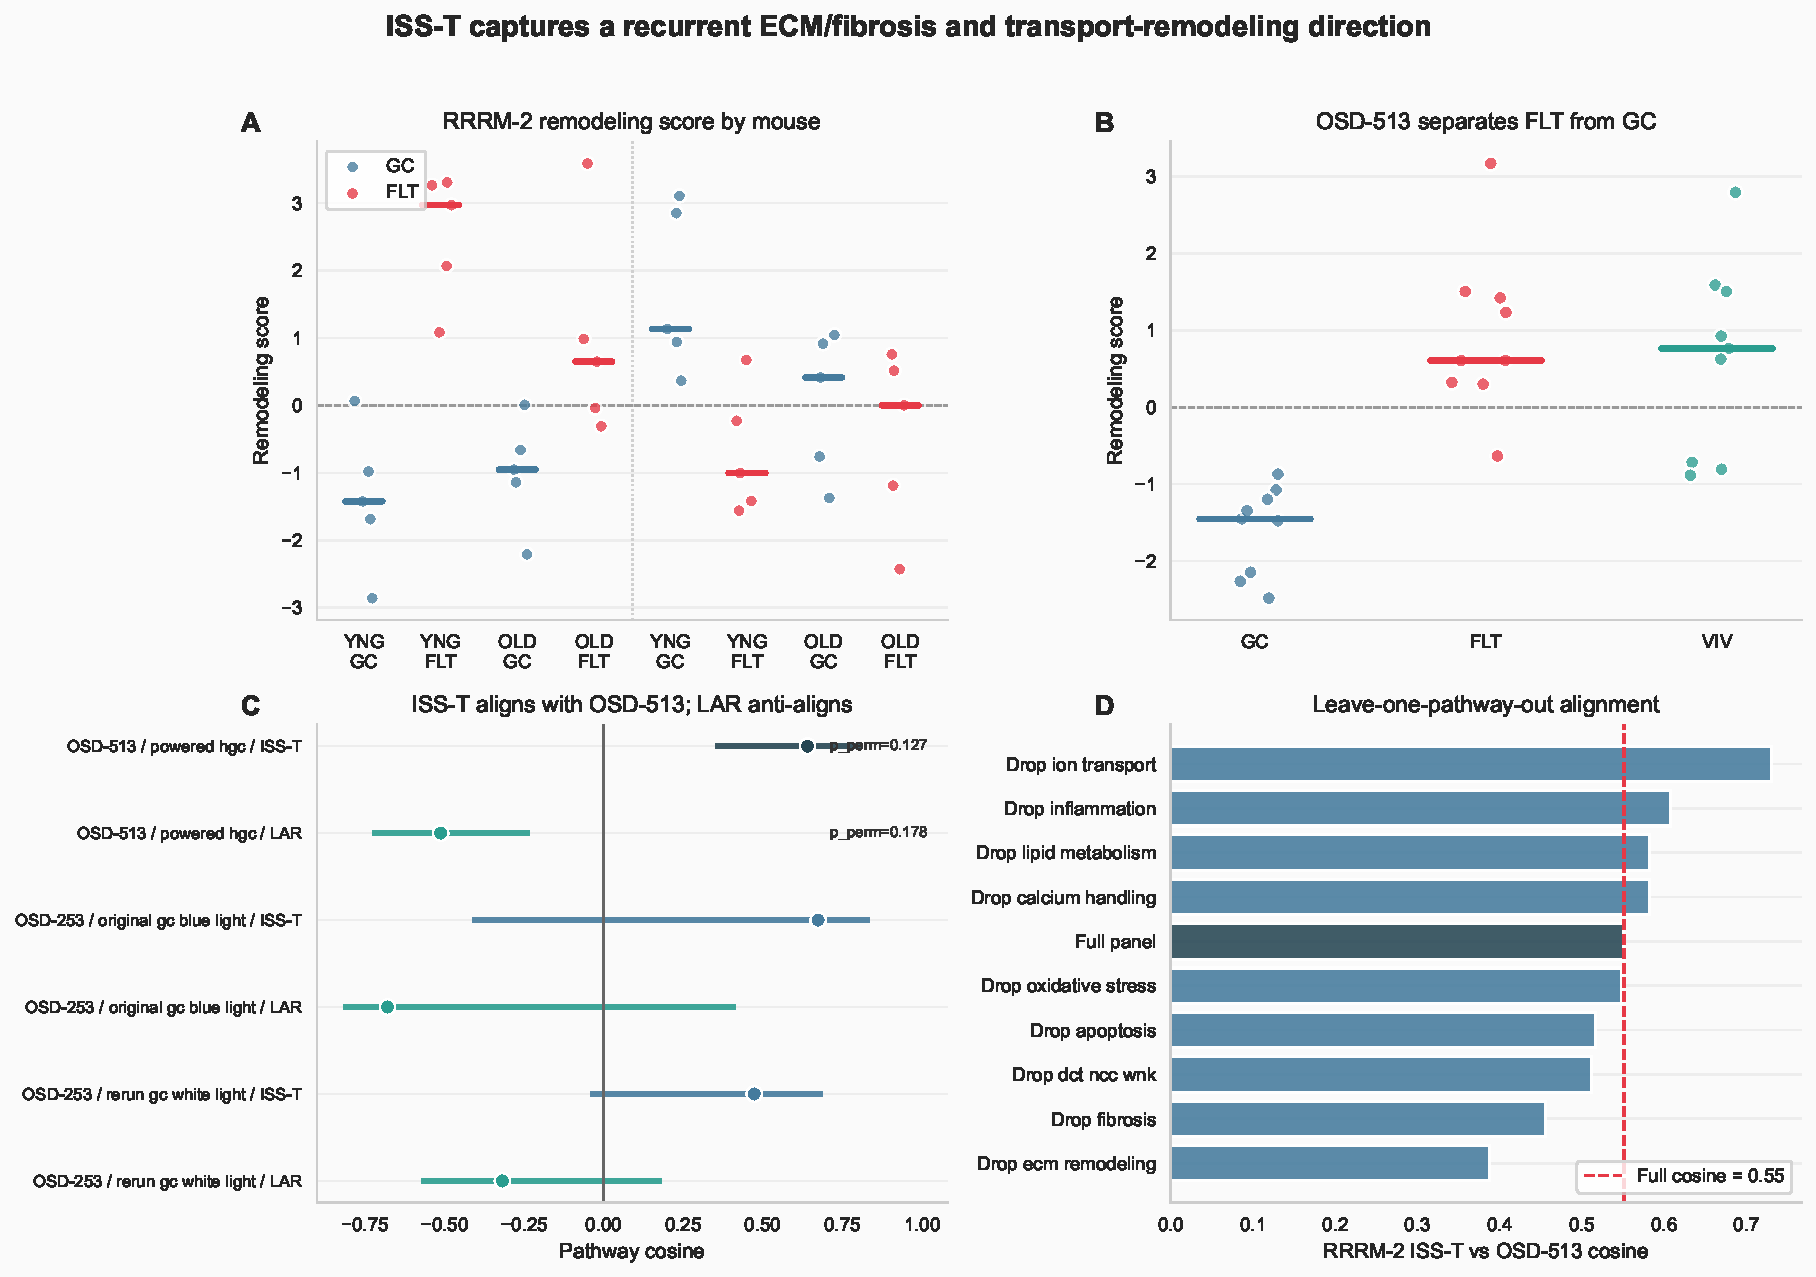
\includegraphics[width=\textwidth]{fig1_main_result_multipanel.pdf}
\caption{\textbf{Main result overview.} (A) RRRM-2 mouse-level remodeling scores by arm, age, and flight group. Points are individual mice; colored bars are group medians. (B) OSD-513 mouse-level separation on the same remodeling score. (C) Cross-OSDR pathway-vector alignment shows ISS-T alignment with OSD-513 and LAR anti-alignment. (D) Leave-one-pathway-out analysis shows that the alignment is not driven by a single pathway alone.}
\label{fig:mainresult}
\end{figure}

\subsection{ISS-T aligns with OSD-513; LAR anti-aligns}

The strongest positive result was arm-specific cross-OSDR alignment at pathway resolution. The RRRM-2 ISS-T flight vector aligned with the OSD-513 flight vector with cosine 0.641 and bootstrap 95\% CI 0.351 to 0.814. In the label-permutation sensitivity, the OSD-513 ISS-T cosine was above the null median near zero but did not reach a 0.05 directional permutation threshold ($p_{\mathrm{perm}}=0.127$). The RRRM-2 LAR vector was anti-aligned with OSD-513, with cosine $-0.511$, CI $-0.726$ to $-0.231$, and directional permutation $p=0.178$ (Table~\ref{tab:crossosdr}; Figure~\ref{fig:alignment}). OSD-253 C57BL/6J comparisons had positive ISS-T point estimates under both control definitions but wide confidence intervals crossing zero, so OSD-253 was carried forward as mechanism/context rather than recurrence evidence.

\begin{table}[H]
\centering\small
\resizebox{\textwidth}{!}{%
\begin{tabular}{lllrrrrrcc}
\toprule
Study & Scenario & Arm & Point & Median & Lower CI & Upper CI & $p_{\mathrm{perm}}$ & Boundary & Claimable \\
\midrule
OSD-513 & powered HGC & ISS-T & 0.641 & 0.625 & 0.351 & 0.814 & 0.127 & recurrence & yes \\
OSD-513 & powered HGC & LAR & -0.511 & -0.498 & -0.726 & -0.231 & 0.178 & recurrence & no \\
OSD-253 & original GC blue light & ISS-T & 0.674 & 0.602 & -0.411 & 0.836 & 0.141 & context & no \\
OSD-253 & original GC blue light & LAR & -0.679 & -0.608 & -0.816 & 0.415 & 0.125 & context & no \\
OSD-253 & rerun GC white light & ISS-T & 0.474 & 0.470 & -0.040 & 0.688 & 0.269 & context & no \\
OSD-253 & rerun GC white light & LAR & -0.318 & -0.309 & -0.572 & 0.183 & 0.344 & context & no \\
\bottomrule
\end{tabular}
}
\caption{\textbf{Cross-OSDR pathway-vector alignment.} OSD-513 is interpreted as directional recurrence. OSD-253 is interpreted as context sensitivity because of control-scenario caveats. $p_{\mathrm{perm}}$ is the directional external-label permutation sensitivity with the RRRM-2 reference vector held fixed.}
\label{tab:crossosdr}
\end{table}

\begin{figure}[H]
\centering
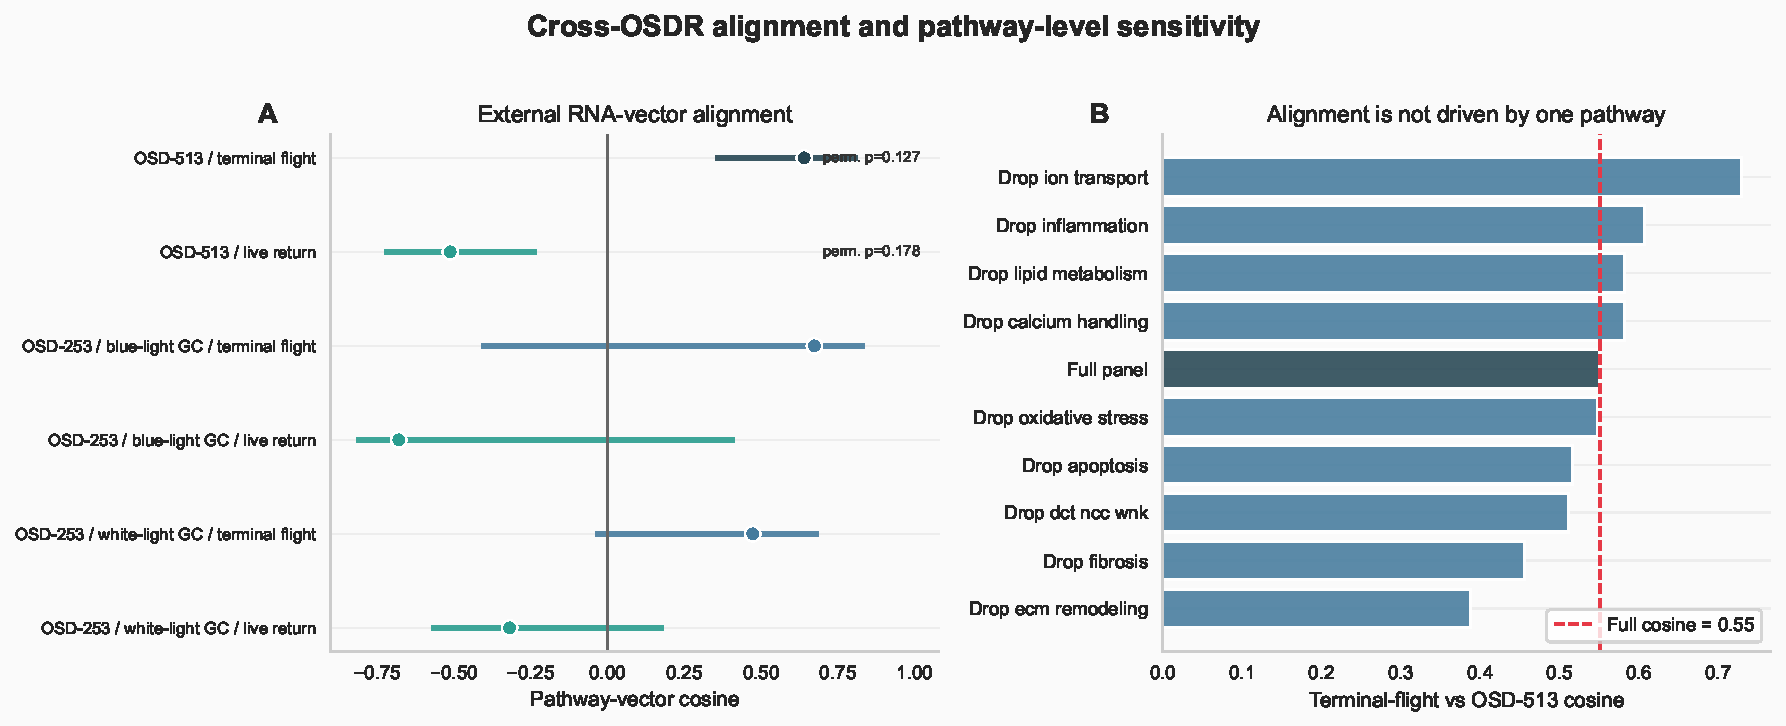
\includegraphics[width=\textwidth]{fig4_cross_alignment_leave_one_out.pdf}
\caption{\textbf{Cross-OSDR alignment and leave-one-pathway-out sensitivity.} (A) RRRM-2 arm-specific flight vectors compared with external OSDR pathway vectors. ISS-T aligns with OSD-513, whereas LAR anti-aligns; OSD-513 labels show directional external-label permutation $p$ values. (B) Leave-one-pathway-out cosines show that the RRRM-2 ISS-T/OSD-513 alignment is distributed across the pathway panel rather than fully dependent on a single component.}
\label{fig:alignment}
\end{figure}

The arm-specific sign pattern is the key biological finding. The terminal-flight arm captures a recurring flight-associated kidney remodeling direction. The return/recovery arm does not recapitulate that direction and is directionally opposite to OSD-513 in the pathway-vector comparison, especially for ECM/fibrosis features. This distinction is consistent with live-return attenuation or context-dependent divergence, while still leaving recovery timing and collection context as linked explanations.

\subsection{The recurrent axis is ECM/fibrosis-positive and DCT/NCC-WNK-negative}

Pathway-level decomposition identified the features that define the recurring ISS-T/OSD-513 direction. Concordant positive pathways were ECM remodeling, fibrosis, apoptosis, and oxidative stress. DCT/NCC-WNK transport was concordantly negative and therefore received a negative weight. Calcium handling, inflammation, broad ion transport, and lipid metabolism were excluded from the primary axis because they were discordant or mixed. Broad ion transport was retained as sensitivity only. The sample-level pathway scores show the same biological direction: ECM organization increases and DCT/NCC-WNK transport decreases most clearly in the RRRM-2 ISS-T and OSD-513 flight comparisons (Figure~\ref{fig:pathwayscores}).

\begin{figure}[H]
\centering
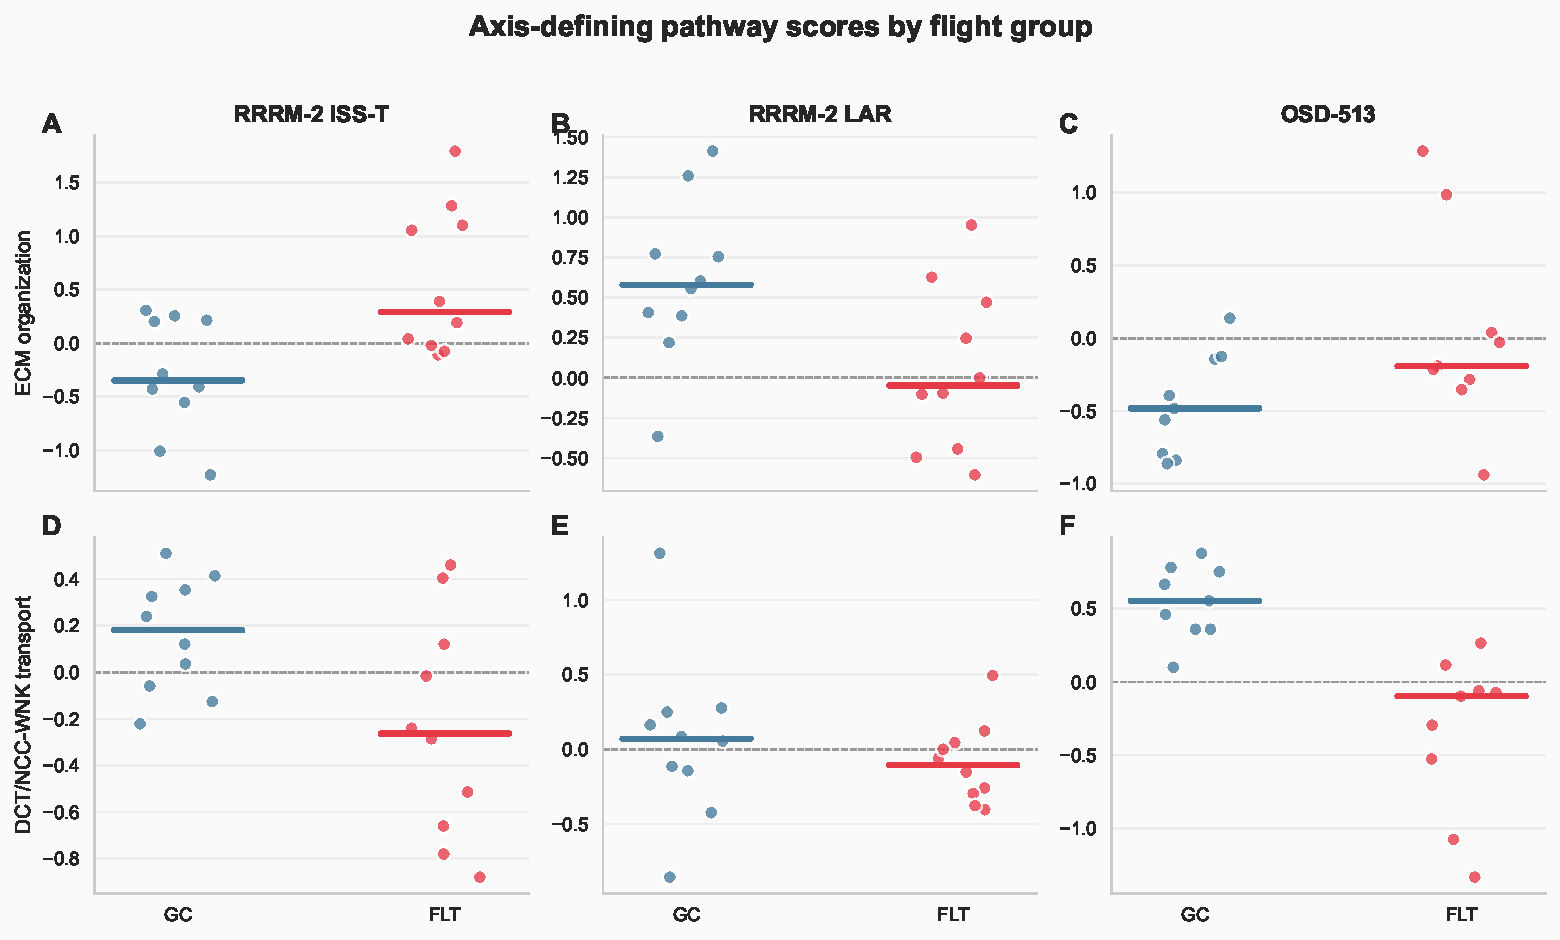
\includegraphics[width=\textwidth]{fig3_pathway_scores_by_flight.pdf}
\caption{\textbf{Axis-defining pathway scores by flight group.} Points are individual mice, and colored bars show medians. ECM organization increases and DCT/NCC-WNK transport decreases in the aligned RRRM-2 ISS-T and OSD-513 flight contexts.}
\label{fig:pathwayscores}
\end{figure}

\begin{table}[H]
\centering\small
\begin{tabular}{lrrrc}
\toprule
Pathway & RRRM-2 ISS-T effect & OSD-513 effect & Axis weight & Primary axis \\
\midrule
ECM remodeling & 0.949 & 0.801 & 0.622 & yes \\
Fibrosis & 0.764 & 0.652 & 0.504 & yes \\
DCT/NCC-WNK & -0.398 & -0.889 & -0.452 & yes \\
Apoptosis & 0.674 & 0.386 & 0.378 & yes \\
Oxidative stress & 0.198 & 0.104 & 0.108 & yes \\
Inflammation & 0.561 & -0.092 & 0.000 & no \\
Ion transport & 0.329 & -0.762 & 0.000 & sensitivity \\
Lipid metabolism & -0.320 & 0.156 & 0.000 & no \\
Calcium handling & 0.003 & -0.550 & 0.000 & no \\
\bottomrule
\end{tabular}
\caption{\textbf{Pathway construction of the recurrent ISS-T remodeling axis.} Effects are pathway-scale FLT-minus-GC contrasts. The final axis is oriented so ECM/fibrosis is positive and DCT/NCC-WNK suppression is negative.}
\label{tab:axisweights}
\end{table}

This axis provides the biological language for the rest of the manuscript: an ECM/fibrosis-positive and DCT/NCC-WNK-negative remodeling score that recurs between RRRM-2 ISS-T and OSD-513.

\subsection{A matrix-high / DCT-low tubulointerstitial state emerges across cohort context}

The recurrent axis can be read more directly as a two-dimensional tissue-state shift. The matrix component summarizes ECM organization, integrin/cell adhesion, and MMP/ADAM proteolysis. The DCT transport component is kept in its native biological direction, so higher values mean stronger DCT/NCC-WNK transport. The remodeling direction is therefore rightward and downward in state space, and the scalar \code{matrix\_minus\_dct} is defined as matrix component minus DCT transport component (Figure~\ref{fig:statespace}).

\begin{figure}[H]
\centering
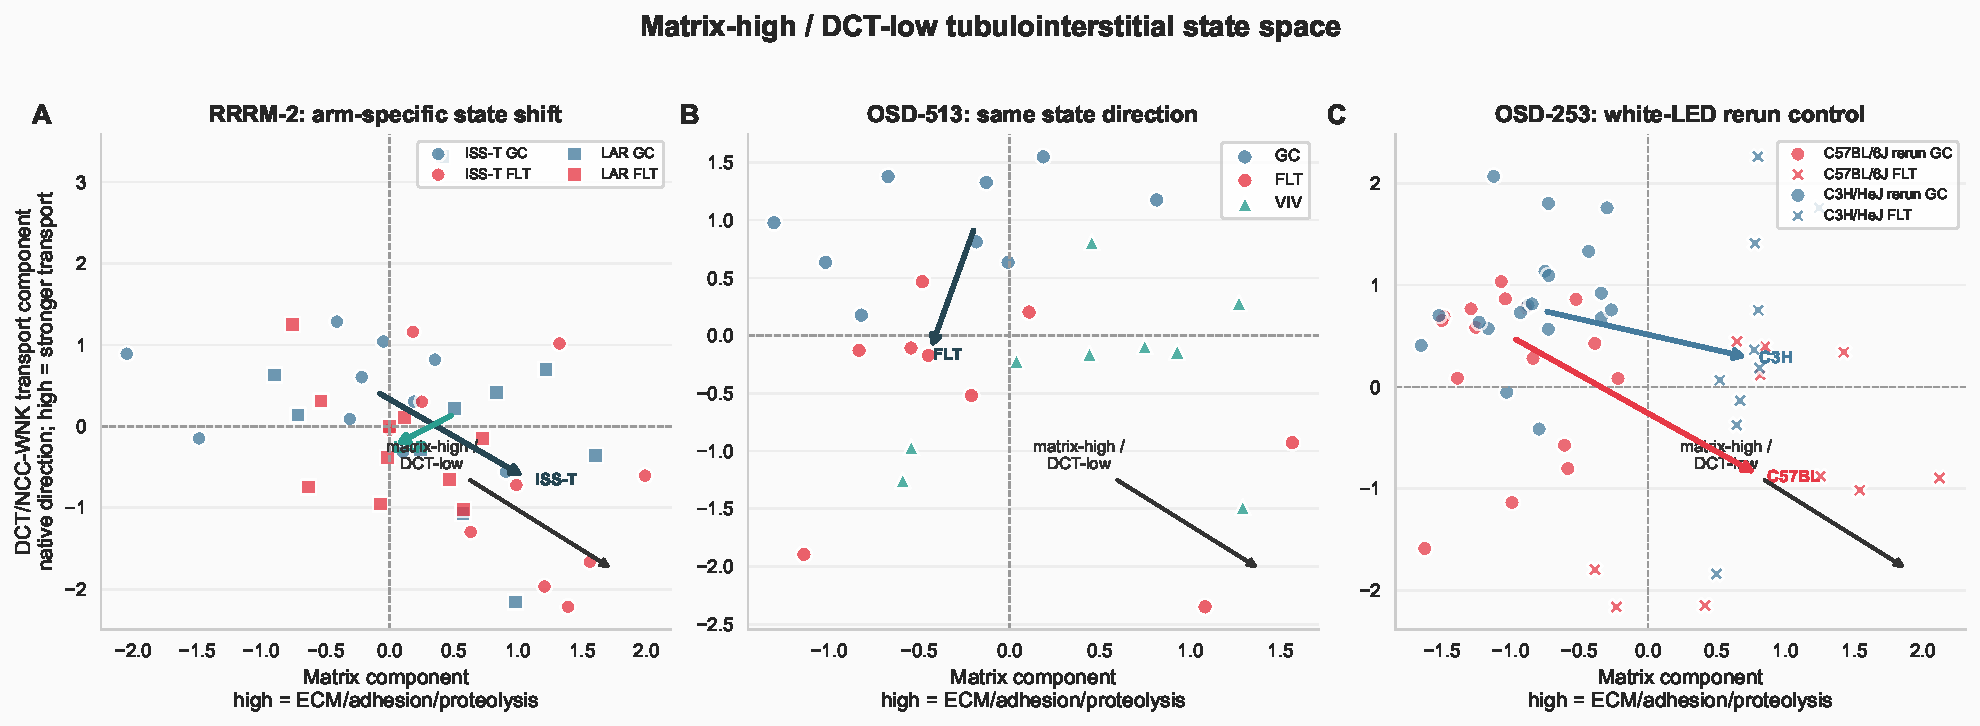
\includegraphics[width=\textwidth]{fig8_tubulointerstitial_state_space.pdf}
\caption{\textbf{Matrix-high / DCT-low tubulointerstitial state space.} The x-axis is the matrix component, where higher values indicate higher ECM/adhesion/proteolysis activity. The y-axis is the DCT/NCC-WNK transport component in native direction, where higher values indicate stronger DCT transport signature. The remodeling direction is rightward and downward. Points are individual mice. Arrows connect group medians from control to flight within the plotted context.}
\label{fig:statespace}
\end{figure}

The state-space effects sharpen the biological interpretation (Figure~\ref{fig:stateeffects}). RRRM-2 ISS-T showed a positive matrix shift (FLT-minus-GC effect $=1.25$, $q=0.0158$), a negative DCT transport shift ($-1.00$, $q=0.102$), and a strong positive matrix-minus-DCT state shift ($2.25$, $q=0.0163$). Immune-context and preservation-stress components were also higher in ISS-T flight ($1.16$, $q=0.0012$; $1.06$, $q=0.0310$). RRRM-2 LAR did not show the same state shift: matrix-minus-DCT was near zero ($-0.11$, $q=0.904$).

OSD-513 was directionally consistent at the scalar state level, with matrix-minus-DCT increasing in flight ($1.81$, $q=0.0310$). This OSD-513 state shift was driven most strongly by DCT/NCC-WNK suppression ($-1.57$, $q=0.0082$), while the matrix component was positive but not significant ($0.25$, $q=0.627$). This distinction matters: OSD-513 supports the same matrix-high/DCT-low direction, but it does not independently reproduce every component with equal strength. The OSD-513 label-permutation caveat remains part of the interpretation.

Under the OSD-253 white-LED rerun control scenario, both strains moved toward the matrix-high/DCT-low state. C57BL/6J showed a strong scalar effect ($2.68$, $q=2.3\times10^{-4}$) with matrix increase ($1.64$, $q=8.7\times10^{-4}$) and DCT decrease ($-1.04$, $q=0.072$). C3H/HeJ also showed a positive scalar effect ($1.82$, $q=0.0031$) and matrix increase ($1.51$, $q=3.1\times10^{-6}$), while its DCT component was only weakly negative ($-0.31$, $q=0.612$). Under the original-GC scenario, the scalar effects were weaker (C57BL/6J $0.79$, $q=0.229$; C3H/HeJ $-0.29$, $q=0.633$), reinforcing that OSD-253 is sensitive to control definition.

\begin{figure}[H]
\centering
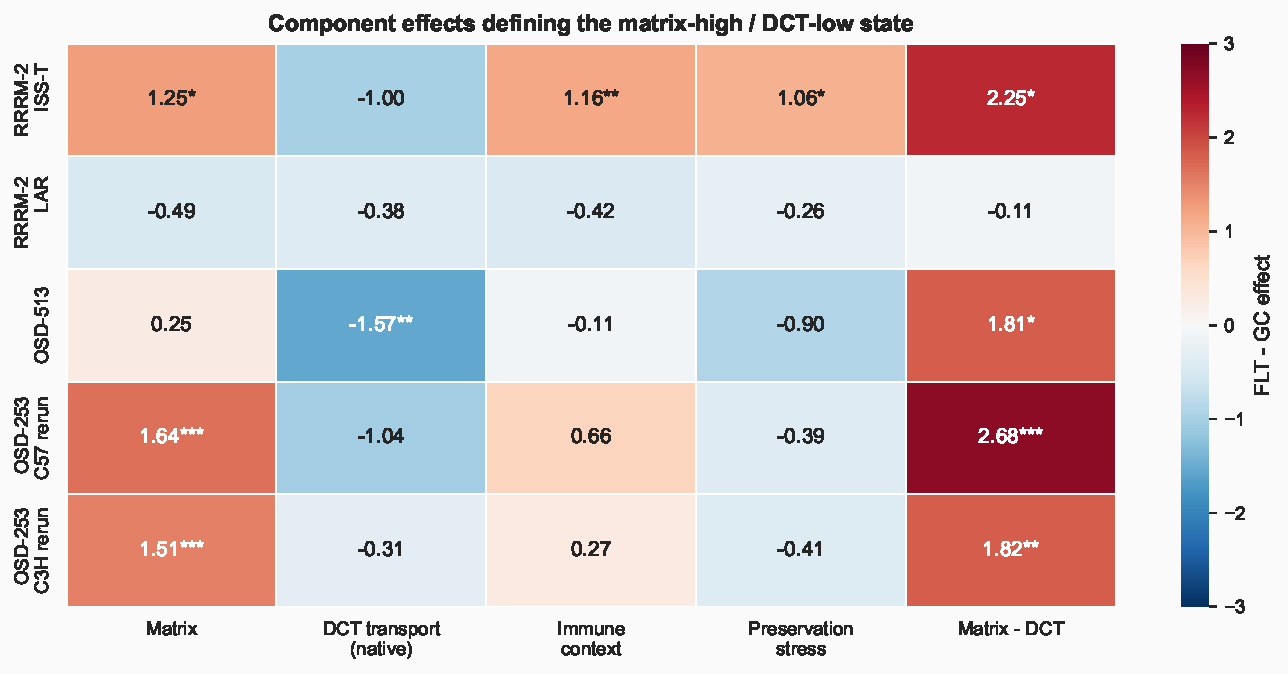
\includegraphics[width=\textwidth]{fig11_state_component_effects.pdf}
\caption{\textbf{Component effects defining the matrix-high / DCT-low state.} Values are FLT-minus-GC effects in standardized component units. Asterisks indicate BH-adjusted thresholds within the component-effect table. DCT transport is shown in native direction, so negative values indicate lower DCT/NCC-WNK transport signature in flight.}
\label{fig:stateeffects}
\end{figure}

RRRM-2 deconvolution estimates did not materially track the state components (Figure~\ref{fig:deconvoverlay}). All 80 RRRM-2 samples joined to the deconvolution table. Across tested state-component/cell-proportion pairs, the largest absolute Spearman correlation was small ($|\rho|=0.120$ for matrix component versus CLR fibroblast estimate), and all BH-adjusted $q$ values were approximately 0.99. Within the available deconvolution model, the matrix-high/DCT-low state is therefore not simply a readout of estimated DCT or fibroblast fraction.

\begin{figure}[H]
\centering
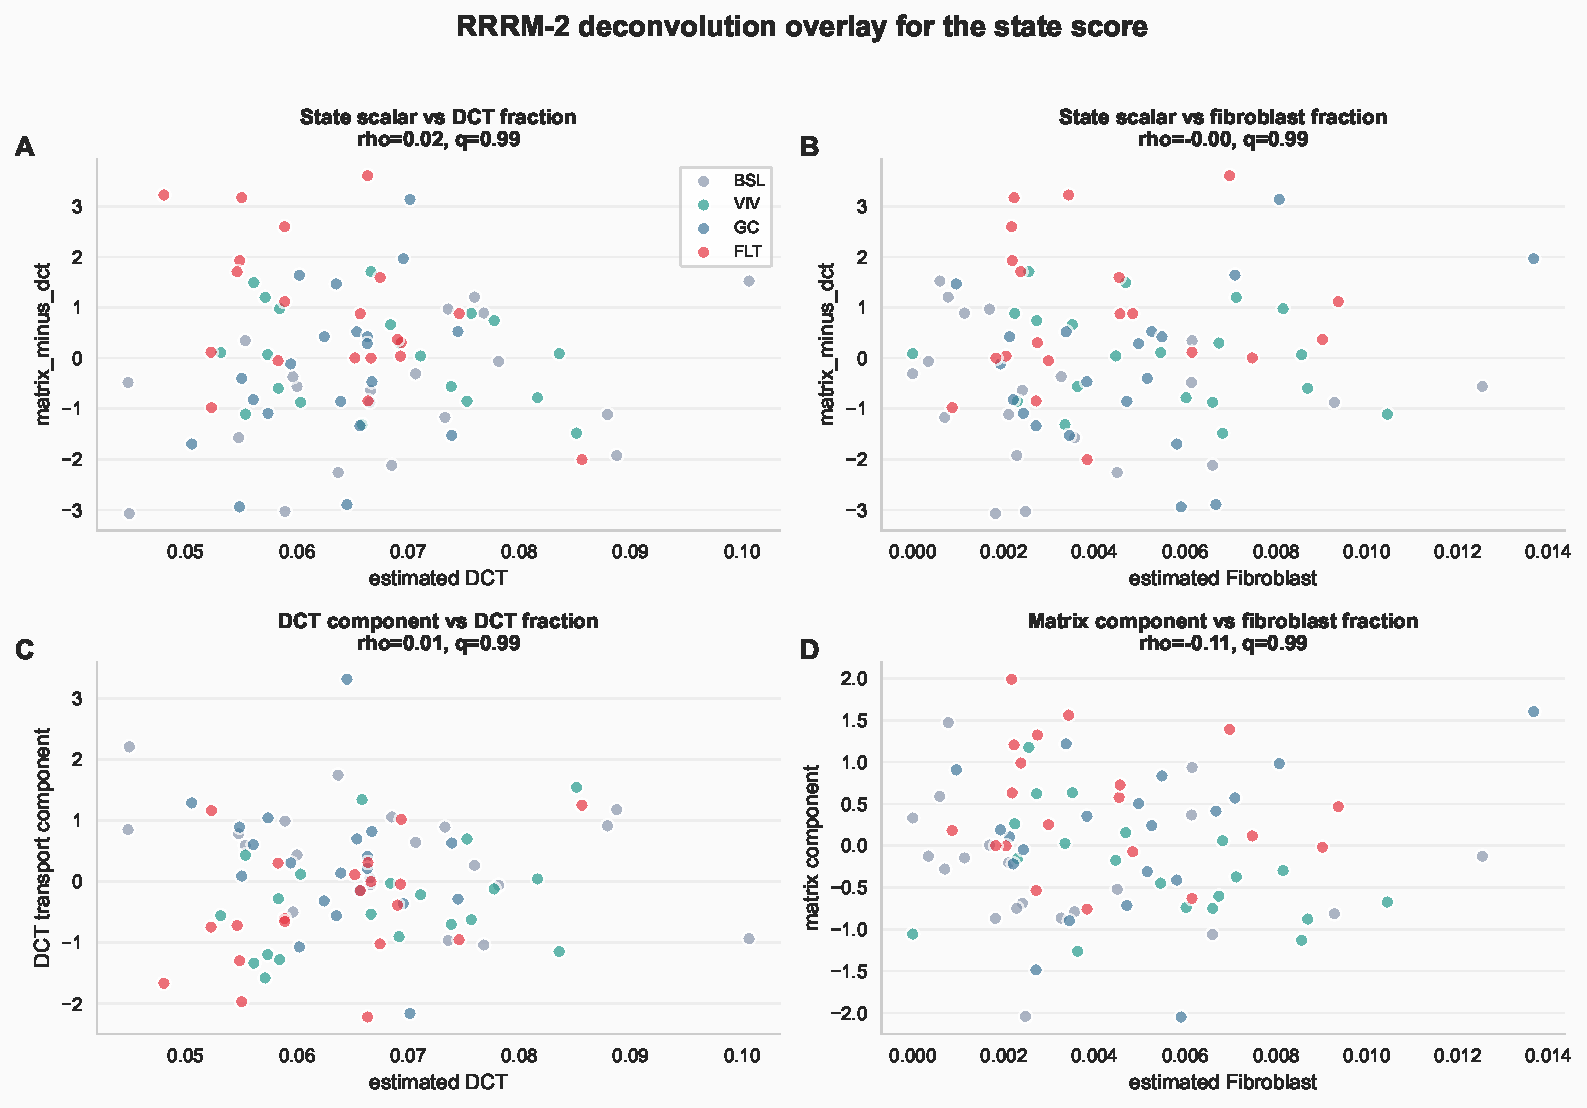
\includegraphics[width=\textwidth]{fig9_rrrm2_deconvolution_overlay.pdf}
\caption{\textbf{RRRM-2 deconvolution overlay for the tubulointerstitial state.} Points are individual RRRM-2 mice. The scalar state score and its components show little correlation with estimated DCT or fibroblast proportions, suggesting that the state-space signal is not explained by these deconvolution estimates alone.}
\label{fig:deconvoverlay}
\end{figure}

Finally, targeted residualized-expression visualization placed familiar renal genes inside the state interpretation (Figure~\ref{fig:renalpanel}). The panel includes 53 scored genes across ECM/adhesion/proteolysis, TLR/innate/macrophage, DCT/NCC-WNK transport, and tubular/metabolic-priority classes. This is a biological annotation display rather than an additional discovery test, but it is useful for seeing that the state-space result is carried by recognizable renal-remodeling and tubular-transport genes.

\begin{figure}[H]
\centering
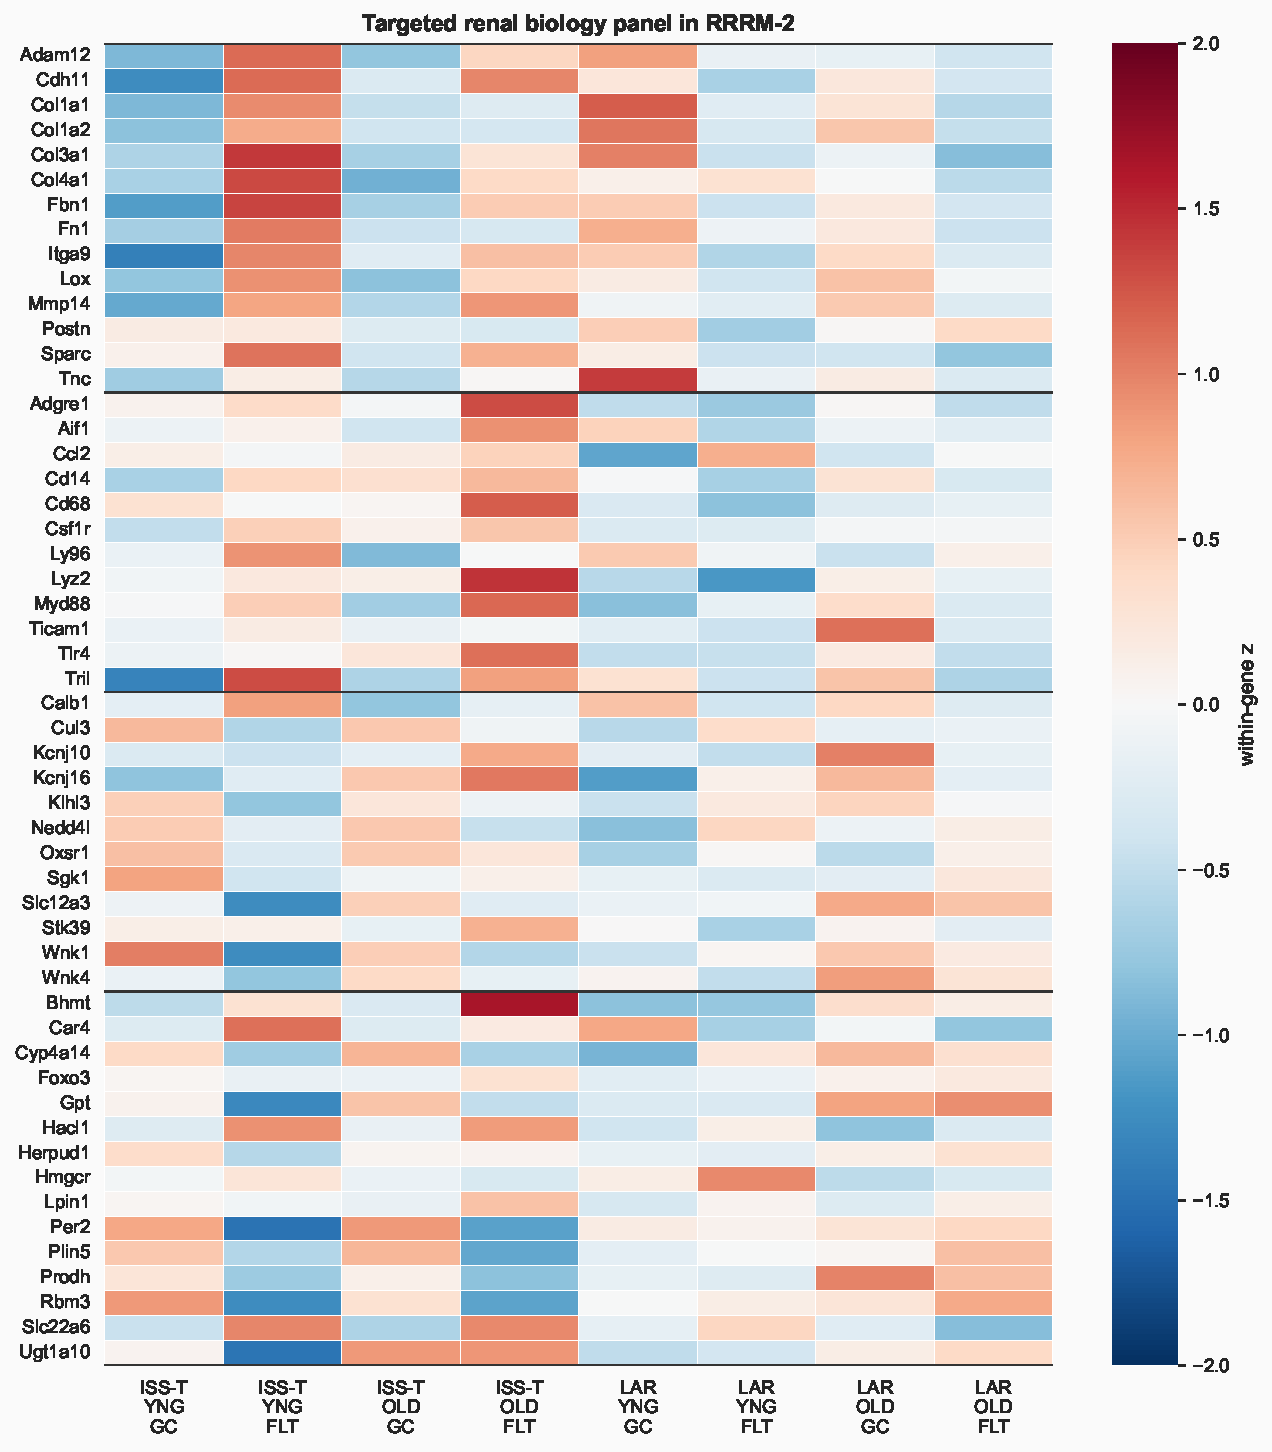
\includegraphics[width=0.95\textwidth]{fig10_targeted_renal_gene_heatmap.pdf}
\caption{\textbf{Targeted renal biology panel in RRRM-2.} Values are group-mean, within-gene z-scores from residualized expression. Rows are grouped by biology class: ECM/adhesion/proteolysis, TLR/innate/macrophage, DCT/NCC-WNK transport, and tubular/metabolic-priority genes.}
\label{fig:renalpanel}
\end{figure}

\subsection{LAR shows attenuation at state-score level and divergence at mechanism-score level}

The LAR arm was next tested against three competing models: attenuation/recovery toward baseline, true reversal of the ISS-T state, and mechanism switch into a different program. After removing the derived \code{matrix\_minus\_dct} scalar from the state-space vector geometry, the pooled LAR state-space vector remained weakly opposite to ISS-T but was unstable (cosine $=-0.564$, bootstrap CI $-0.940$ to $+0.339$, $\beta_{\mathrm{LAR}\rightarrow\mathrm{ISS}}=-0.199$). This supports attenuation rather than a stable state-space reversal. Young LAR had an extreme negative point-estimate cosine (cosine $=-0.982$, directional permutation $p=0.0030$, BH $q=0.0450$), but its bootstrap CI remained wide and crossed zero ($-0.969$ to $+0.559$), so the young state-space direction is not a robust estimate.

\begin{figure}[H]
\centering
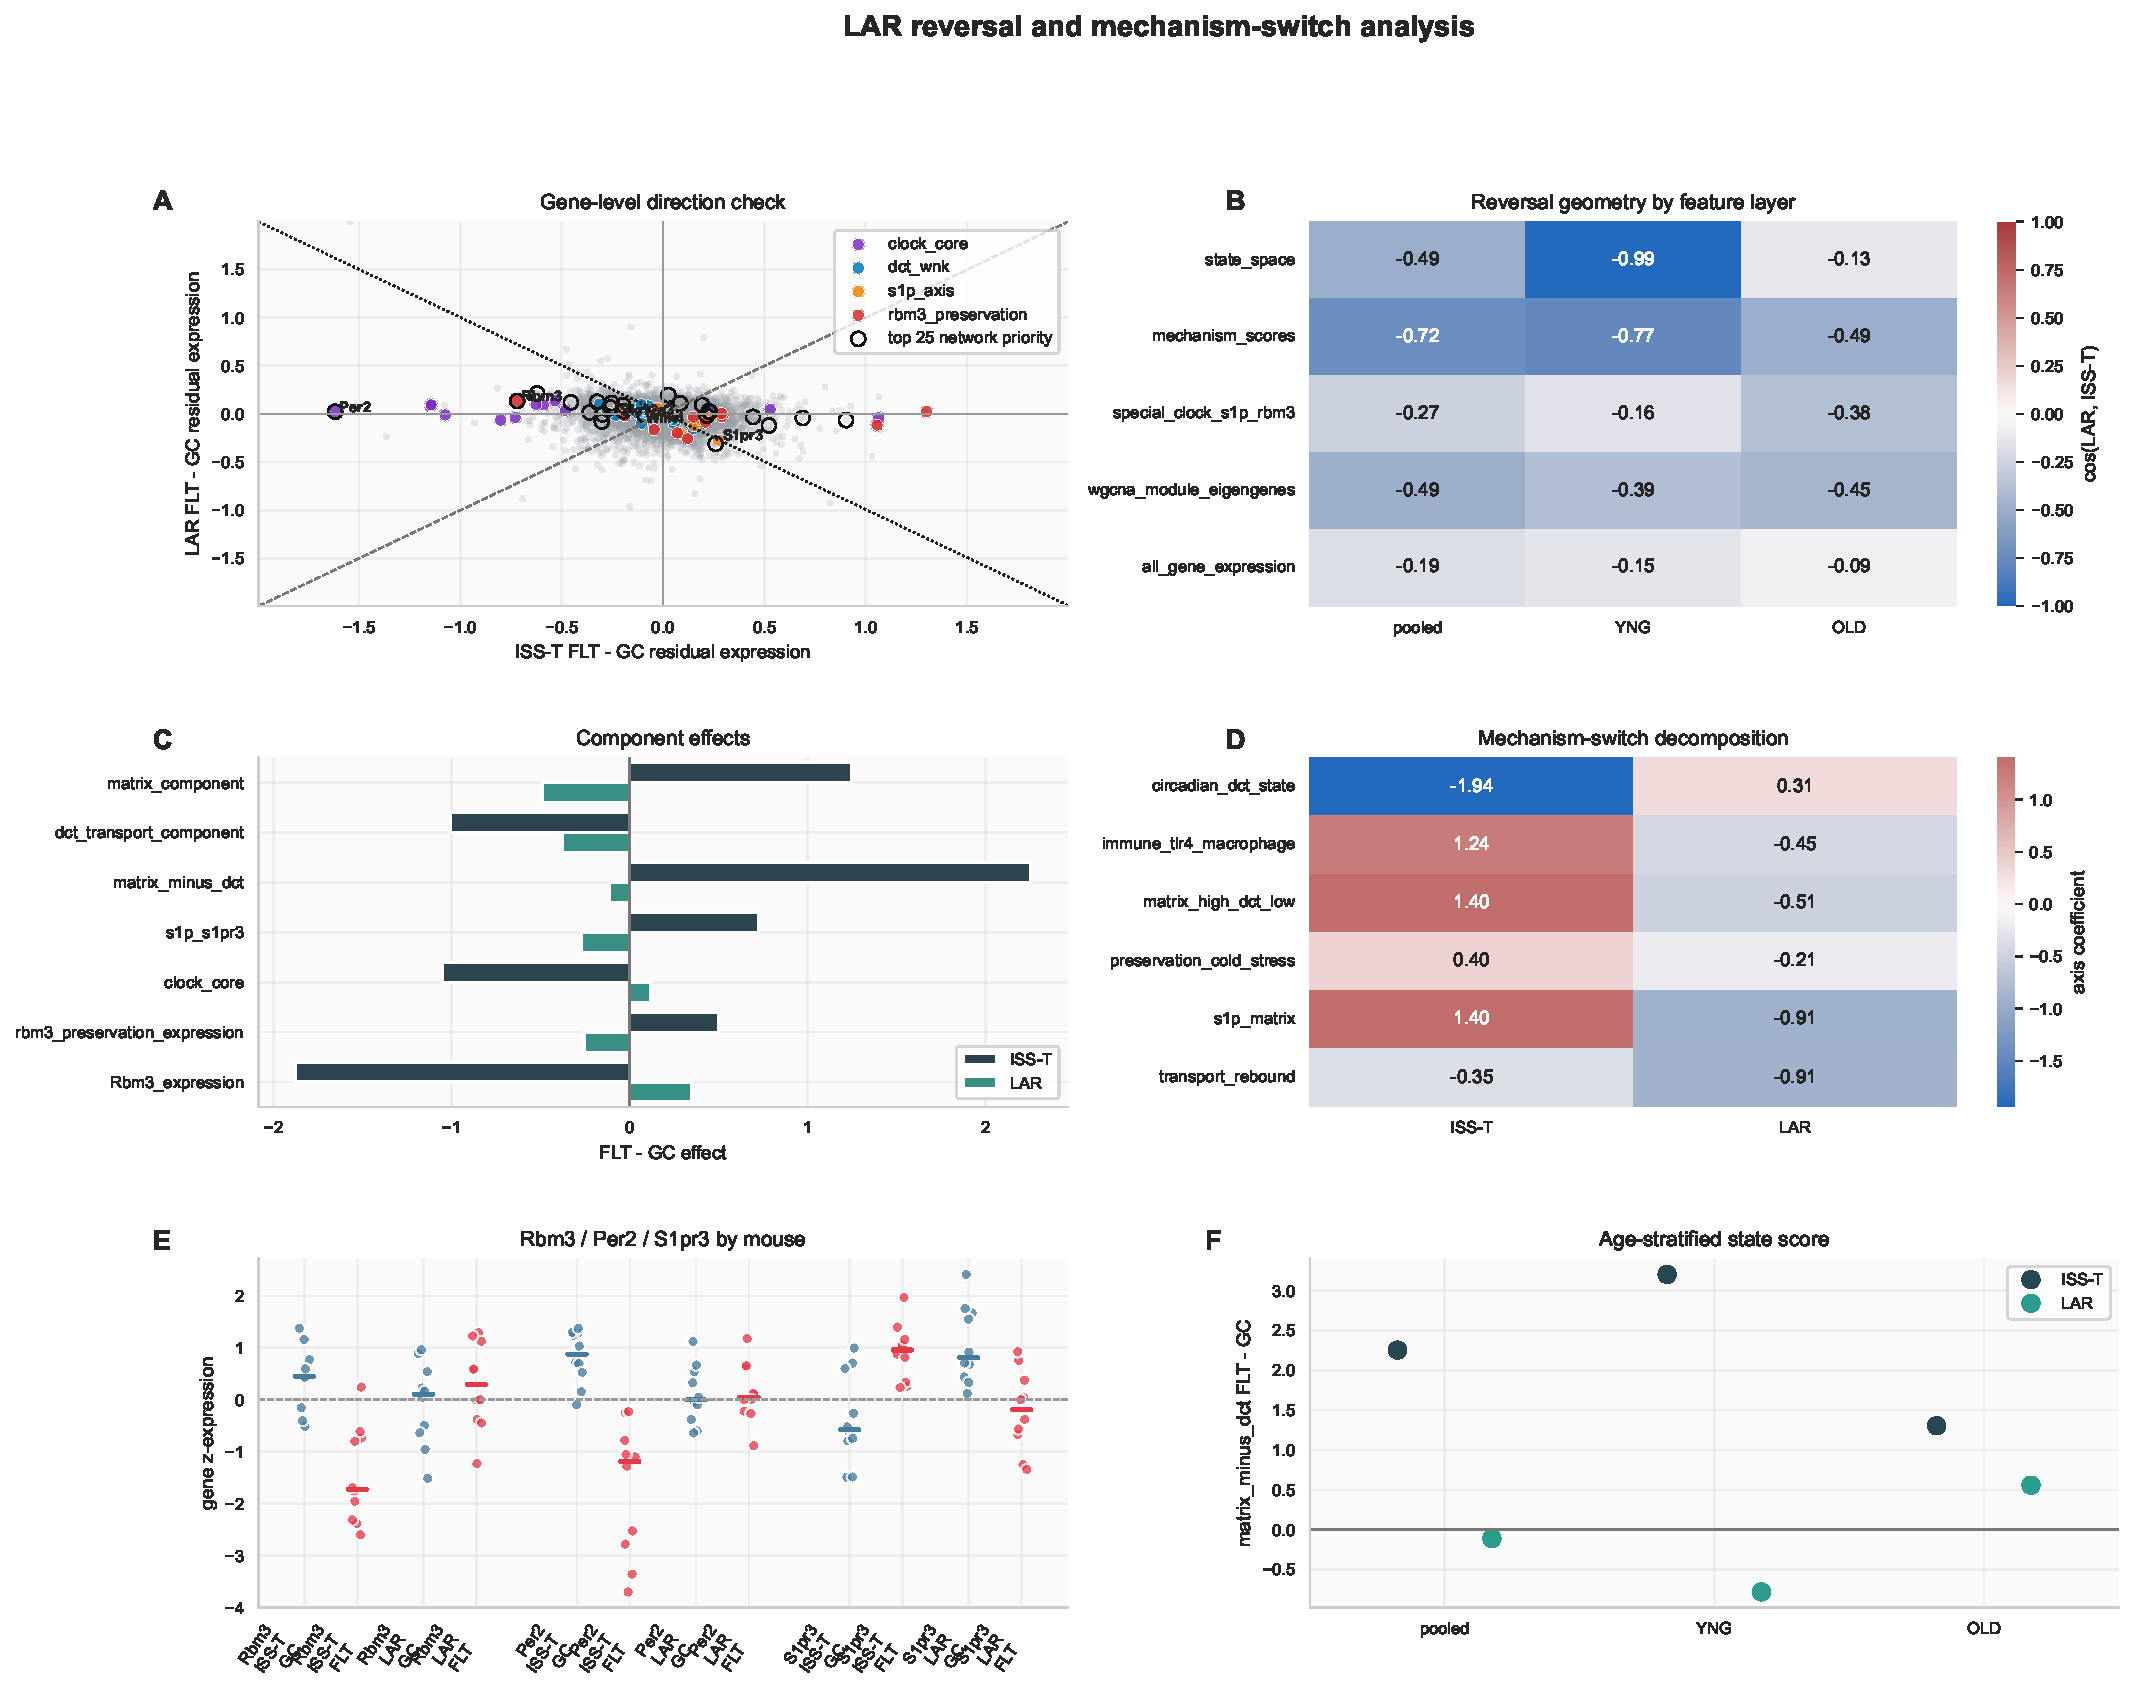
\includegraphics[width=\textwidth]{fig12_lar_reversal_dashboard.pdf}
\caption{\textbf{LAR attenuation/divergence and mechanism-context dashboard.} Panel A shows RRRM-2 ISS-T and LAR gene-level FLT-minus-GC effects, with curated renal biology classes highlighted. Panel B summarizes cosine alignment across feature sets. Panel C shows arm-specific component effects. Panel D projects ISS-T and LAR effects onto exploratory mechanism-context axes. Panel E shows targeted \gene{Rbm3}, \gene{Per2}, and \gene{S1pr3} expression effects. Panel F shows age-stratified matrix-minus-DCT state effects. The visually prominent young-LAR opposite point estimate is interpreted as hypothesis-generating because the LAR effect itself is not statistically distinguishable from zero.}
\label{fig:larreversal}
\end{figure}

The scalar state-score effects are most consistent with ISS-T response and LAR attenuation. Young ISS-T moved strongly toward the matrix-high/DCT-low state (matrix-minus-DCT effect $=+3.204$, BH $q=0.025$), while young LAR had an opposite point estimate ($-0.782$) that was not statistically distinguishable from zero (Welch $p=0.361$, BH $q=0.542$). Old ISS-T showed a weaker positive shift ($+1.304$), and old LAR was weakly positive ($+0.558$). At the pooled level, ISS-T showed a strong state shift ($+2.254$, BH $q=0.020$), whereas LAR was approximately zero ($-0.112$, BH $q=0.895$). The pooled arm-by-flight interaction for the matrix-minus-DCT state was positive and significant (interaction $=2.366$, bootstrap CI $0.865$ to $3.851$, permutation $p=0.0160$, BH $q=0.0267$), but this interaction is driven by ISS-T response against an attenuated LAR response, not by a confirmed non-zero LAR reversal.

Component interactions identify which biology differs most between arms. Matrix was the most robust component: ISS-T increased and LAR decreased the matrix component at the point-estimate level (interaction $=1.738$, BH $q=0.0037$), although the LAR matrix effect itself had a bootstrap interval crossing zero. DCT transport was lower in ISS-T and also lower in pooled LAR, and the pooled DCT interaction was not significant (BH $q=0.346$). Thus, LAR does not show clear DCT recovery.

Mechanism-score vectors provided the strongest evidence that LAR diverges from ISS-T beyond simple state-score attenuation. Pooled mechanism-score vectors showed LAR opposite to ISS-T (cosine $=-0.725$, bootstrap CI $-0.874$ to $-0.122$, directional permutation $p=0.0160$, BH $q=0.0800$). The clearest component-level divergences involved ECM organization, TLR4/innate signaling, S1P/S1PR3, and \gene{S1pr3} expression. S1P/S1PR3 increased in ISS-T and decreased in LAR (interaction $=0.997$, BH $q=0.0027$), and \gene{S1pr3} expression showed strong arm divergence (ISS-T effect $=+1.276$, LAR effect $=-1.269$, interaction $=2.545$, BH $q=0.0020$).

Clock-associated DCT features nominate a second follow-up axis. Core clock score decreased in ISS-T but was slightly positive in LAR (interaction $=-1.170$, BH $q=0.0020$); the Per/Cry subscore showed the same arm divergence (interaction $=-2.061$, BH $q=0.0024$). \gene{Per2} decreased strongly in ISS-T and was approximately unchanged in LAR (interaction $=-2.563$, BH $q=0.0024$). Across RRRM-2 samples, \gene{Per2} expression correlated positively with the DCT transport component ($\rho=0.449$, BH $q=7.5\times10^{-5}$) and negatively with matrix-minus-DCT ($\rho=-0.547$, BH $q=7.6\times10^{-7}$). Because RRRM-2 does not provide a time-series design or sufficient time-of-day metadata for phase inference, this result is described as a clock-gene-associated transcriptional state, not a measured circadian phase shift.

Exploratory mechanism-axis projections were retained as context, not as confirmatory decomposition. The hand-defined axes explained 37\% of the ISS-T mechanism-feature variance and 51\% of the LAR variance, leaving substantial residual signal. Their coefficients are therefore useful as biological sketches: matrix/S1P/innate features point toward ISS-T-positive/LAR-negative biology, clock-DCT features suggest ISS-T suppression with LAR attenuation or partial rebound, and transport-rebound features remain negative in both arms. These projections nominate mechanisms to test, but they do not establish three separable programs as a primary result.

At broader feature levels, WGCNA module eigengenes also pointed oppositely (pooled cosine $=-0.489$, bootstrap CI $-0.763$ to $-0.080$), though permutation support was weaker. All-gene expression was much weaker (cosine $=-0.187$), arguing against a genome-wide reversal. Node2vec displacement magnitudes were moved to a separate context table because magnitude vectors are non-directional and not comparable to signed effect vectors. Therefore, the LAR result is best framed as pooled attenuation with mechanism-level divergence, plus an underpowered age-stratified observation that may motivate validation.

\subsection{Mechanism scores nominate ECM, innate, adhesion, S1P, and DCT programs}

Mechanism scoring asked which candidate upstream or contextual programs track the scalar remodeling score. In RRRM-2, the remodeling score correlated strongly with ECM organization ($\rho=0.644$, $q=7.4\times10^{-10}$), DCT/NCC-WNK transport suppression ($\rho=-0.560$, $q=3.1\times10^{-7}$), TLR4/innate signaling ($\rho=0.488$, $q=1.8\times10^{-5}$), MMP/ADAM proteolysis ($\rho=0.478$, $q=2.6\times10^{-5}$), S1P/S1PR3 signaling ($\rho=0.451$, $q=8.2\times10^{-5}$), and integrin/cell adhesion ($\rho=0.374$, $q=1.5\times10^{-3}$). OSD-513 reproduced the ECM-positive and DCT-negative relationship: ECM organization correlated with the remodeling score ($\rho=0.745$, $q=2.7\times10^{-5}$), and DCT/NCC-WNK transport correlated negatively ($\rho=-0.676$, $q=2.8\times10^{-4}$). OSD-253, across all samples, showed strong associations of the remodeling score with TLR4/innate signaling, ECM organization, macrophage/inflammatory context, DCT/NCC-WNK suppression, and S1P/S1PR3 (Figure~\ref{fig:mechheat}).

\begin{figure}[H]
\centering
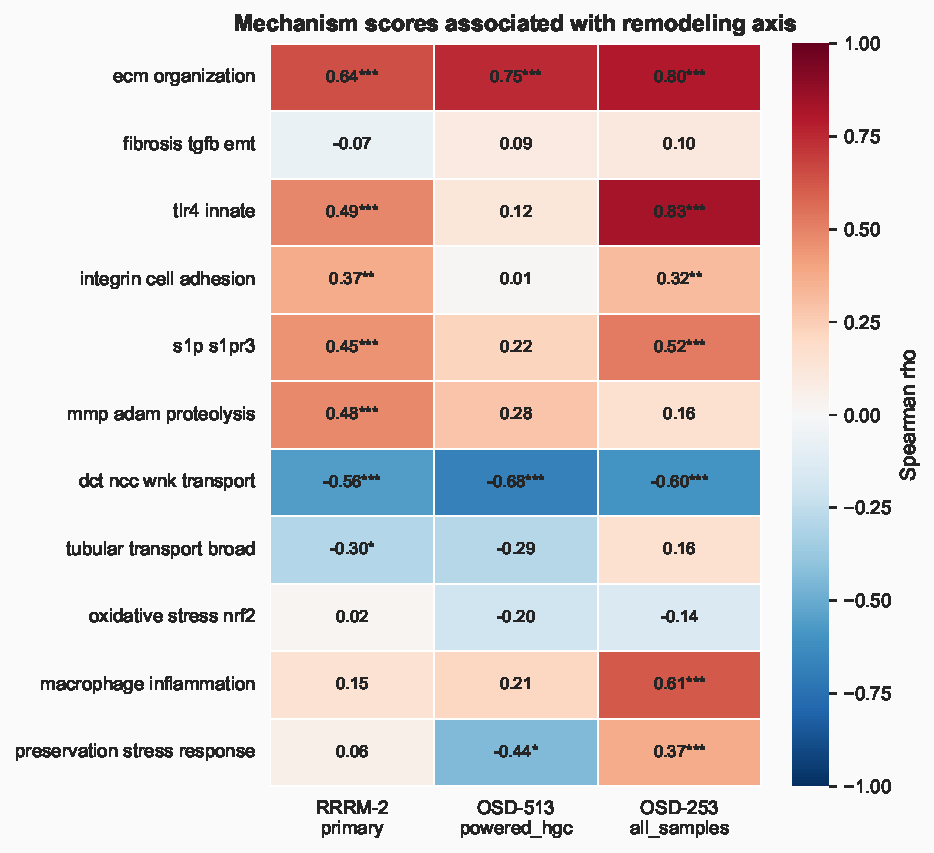
\includegraphics[width=0.82\textwidth]{fig6_mechanism_score_heatmap.pdf}
\caption{\textbf{Mechanism-score associations with the recurrent remodeling score.} Color indicates Spearman correlation between each mechanism score and the scalar remodeling score. Asterisks mark BH-adjusted $q<0.05$ within the association table. RRRM-2 and OSD-513 both show ECM-positive and DCT/NCC-WNK-negative structure. OSD-253 shows strong TLR4/innate, ECM, macrophage/inflammation, and transport relationships across its broader sample set.}
\label{fig:mechheat}
\end{figure}

The mechanism pattern is biologically plausible. TLR4 signaling is implicated in renal inflammation and fibrosis, and TLR4-mutant mice have been reported to be protected from chronic kidney disease progression and renal fibrosis \citep{souza2015tlr4}. TRIL is a co-receptor associated with TLR3/TLR4 signaling and cytokine production \citep{carpenter2009tril,wochal2014tril,carpenter2011tril}. Cadherin-11 has a recognized role in tissue fibrosis and fibroblast-like cell adhesion \citep{chavula2022cadherin}. Integrins and MMP/ADAM proteases are core mediators of cell-matrix adhesion and matrix turnover. Sphingosine-1-phosphate signaling, including S1PR3-centered biology, has been linked to kidney injury, inflammation, and fibrotic remodeling in several contexts \citep{s1p2017,s1p2020}. The DCT/NCC-WNK direction is also coherent with distal nephron transport regulation, where WNK-SPAK/OSR1-NCC signaling governs sodium-chloride cotransport and potassium-sensitive distal nephron physiology \citep{castaneda2024dct,ge2016wnk}.

The mechanism scores place the recurrent remodeling direction in a molecular neighborhood involving ECM deposition, adhesion/proteolysis, innate immune signaling, S1P biology, macrophage/inflammatory context, and tubular transport suppression. This supports a mechanism-prioritization model in which multiple upstream and downstream programs are carried forward for targeted validation.

\subsection{OSD-253 points to TLR4/innate association rather than TLR4 requirement}

OSD-253 was used as the immediate mechanistic discriminator because C3H/HeJ mice have impaired TLR4 signaling. A strict TLR4-dependent model predicts attenuation of the remodeling score in C3H/HeJ relative to C57BL/6J. The observed pattern supports an association model (Figure~\ref{fig:osd253}). Under the original GC blue-light scenario, C57BL/6J remodeling was positive (0.816) and C3H/HeJ remodeling was lower (0.328), with a strain-delta confidence interval crossing zero. Under the white-LED rerun scenario, remodeling was positive in both strains (C57BL/6J 1.379, C3H/HeJ 0.668), again with a strain-delta confidence interval crossing zero. ECM, fibrosis/TGF-beta, integrin/cell adhesion, and MMP/ADAM scores remained positive in C3H/HeJ under the rerun scenario.

\begin{figure}[H]
\centering
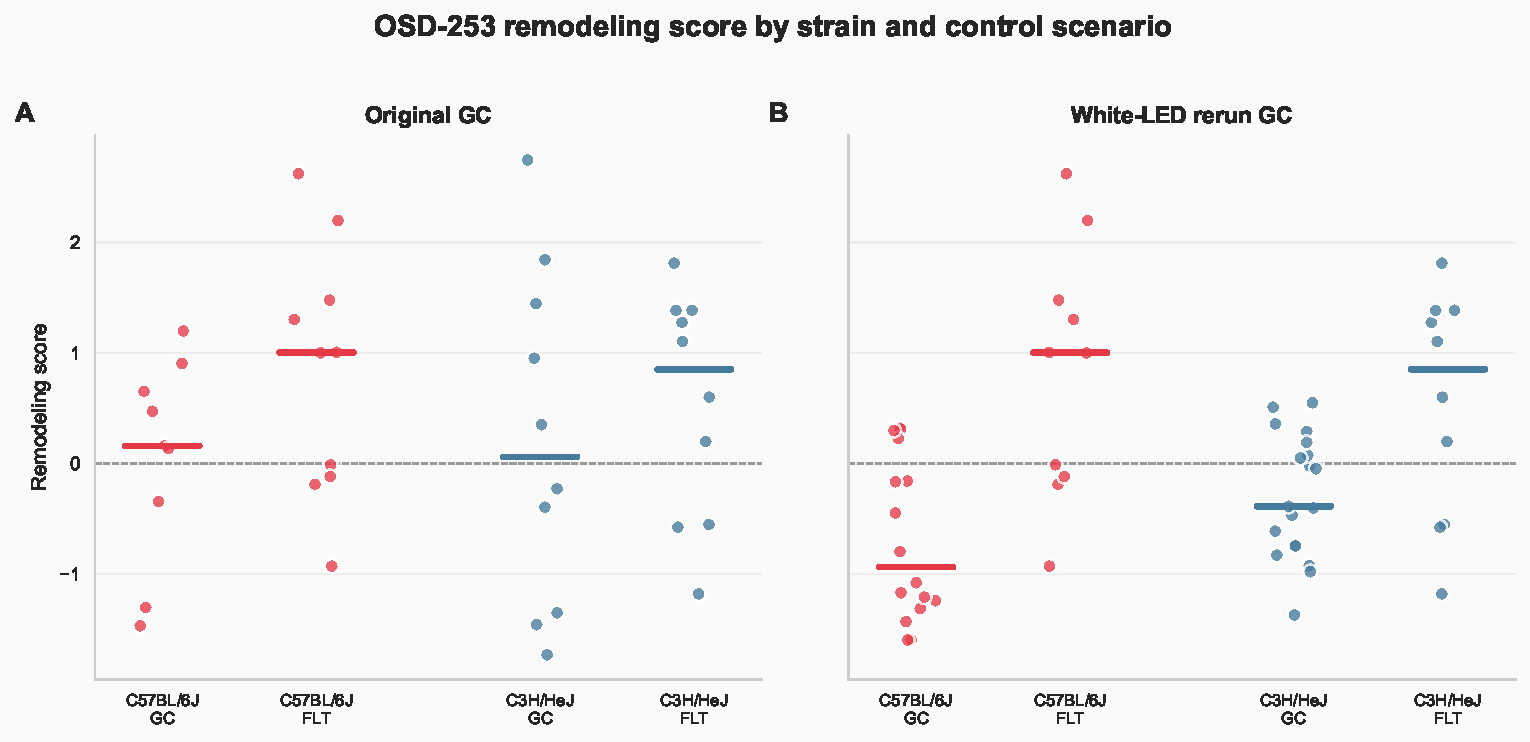
\includegraphics[width=\textwidth]{fig5_osd253_strain_points.pdf}
\caption{\textbf{OSD-253 remodeling score by strain and control scenario.} Points are individual mice, and colored bars show medians. The remodeling score is lower in C3H/HeJ at the point-estimate level, but the program remains positive under the white-LED rerun control scenario.}
\label{fig:osd253}
\end{figure}

TLR4/innate signaling tracks the remodeling score strongly, especially in OSD-253, and remains a plausible contextual axis. The strain comparison favors a TLR4-associated but broader remodeling program. Other mechanisms, including TGF-beta/EMT, adhesion, proteolysis, S1P signaling, macrophage context, and preservation stress, remain plausible contributors or covariates.

\subsection{WGCNA provides structural annotation of the remodeling program}

The WGCNA module layer annotates the remodeling program. A prior WGCNA analysis identified grey60 as a 48-gene ECM/cell-migration module with an ISS-T-specific eigengene pattern and hub structure involving genes such as \gene{Tril}, \gene{Itga9}, \gene{Fbn1}, \gene{S1pr3}, \gene{Cdh11}, \gene{Adam12}, and \gene{Mmp14}. That hub composition is consistent with the mechanism-axis result.

Follow-up overlap analyses place grey60 inside a broader multi-module response. The 11 ISS-T-Young LIONESS factorial edge-rewiring candidates distributed across purple, turquoise, yellow, black, brown, and one off-panel feature. Silent-shifter candidates enriched midnightblue in ISS-T-Young (11/185; $q=0.0031$) and purple in ISS-T-Old (13/171; $q=0.030$). Module eigengene contrasts showed an ISS-T-specific pattern in grey60, royalblue, salmon, and pink. WGCNA therefore supports structural annotation of a multi-module remodeling response, with grey60 as the most biologically interpretable ECM/cell-migration module.

\subsection{LIONESS/node2vec prioritizes candidate local-neighborhood contributors}

The exploratory LIONESS/node2vec ranking asked which genes show ISS-T-specific local network-neighborhood movement, stronger ISS-T node-strength effects than LAR, and support from OSD-513. In the 2,500-gene production run, the top composite genes included \gene{Rbm3}, \gene{Cyp4a14}, \gene{Bhmt}, \gene{Per2}, \gene{Hmgcr}, \gene{Sim2}, \gene{Hacl1}, \gene{Plin5}, \gene{Gpt}, \gene{Prodh}, and \gene{Ugt1a10}. In the 5,000-gene sensitivity run, high-ranking genes included \gene{Rbm3}, \gene{Bhmt}, \gene{Kank3}, \gene{Ugt1a10}, \gene{Ptpn1}, \gene{Serpinb8}, \gene{Cd200}, \gene{Per2}, and \gene{Cyp4a14}.

These genes are candidate local-neighborhood contributors to the pathway-level program. Top-k mechanism enrichment was weak after FDR correction (Figure~\ref{fig:genesens}). In the 2,500-gene production run, the strongest top-k findings were broad tubular transport at top 250 (2/4 genes; fold enrichment 5.0; raw $p=0.052$; $q=0.384$) and preservation stress at top 250 (3/10; fold enrichment 3.0; raw $p=0.070$; $q=0.384$). Ranked-list enrichment suggested broad tubular transport enrichment in the composite score (raw $p=0.0085$, $q=0.076$). In the 5,000-gene sensitivity run, the best ranked-list signals were preservation stress, broad tubular transport, and oxidative stress, all with $q=0.130$ or weaker.

\begin{figure}[H]
\centering
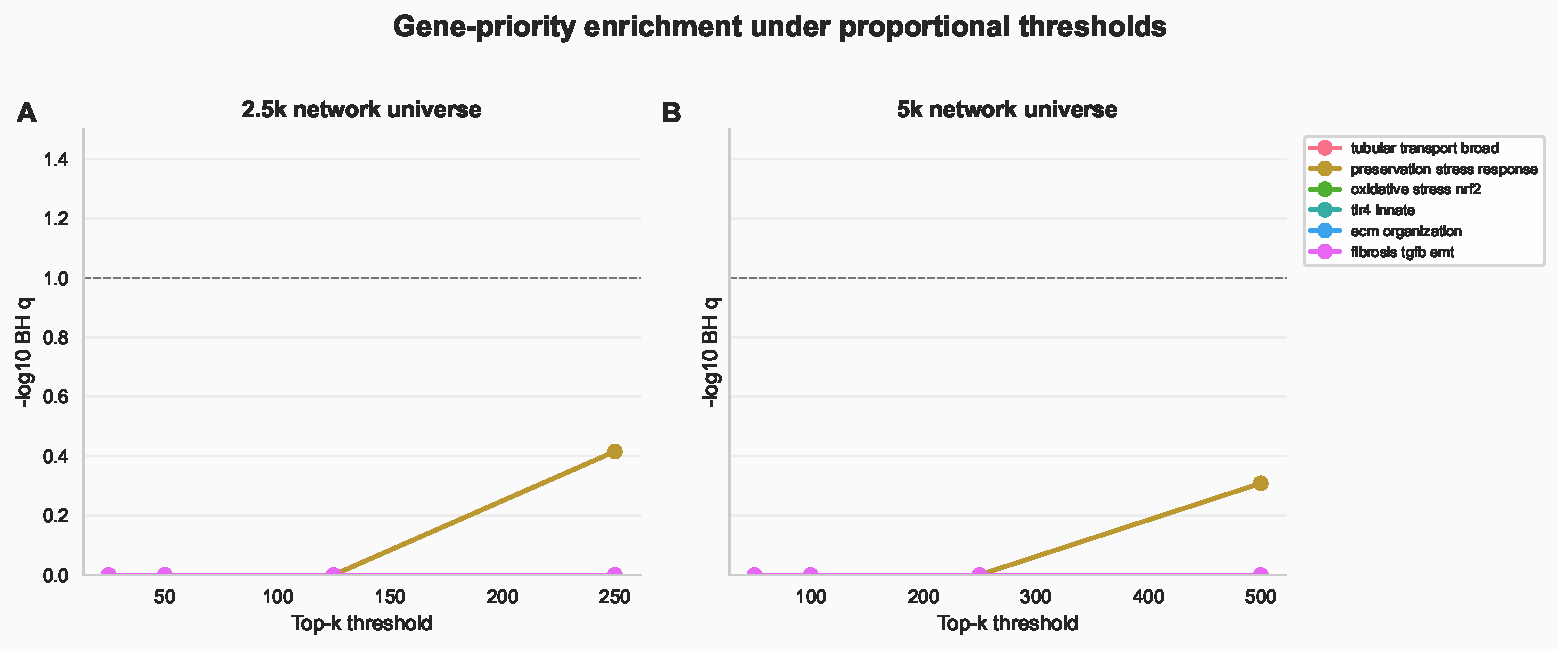
\includegraphics[width=\textwidth]{fig7_gene_priority_sensitivity.pdf}
\caption{\textbf{Top-k sensitivity for LIONESS/node2vec gene prioritization.} The gene-priority layer nominates candidate local-neighborhood contributors. The most consistent weak signals involve broad tubular transport, preservation stress, and oxidative/NRF2 context, while FDR support remains below the pathway/module-scale evidence.}
\label{fig:genesens}
\end{figure}

Node2vec and LIONESS add a gene-prioritization layer: they rank genes whose local network context moves with the ISS-T remodeling program. This layer is useful for follow-up target selection and gene-level annotation of the pathway/module result.

\subsection{External aging-axis projection favors remodeling over aging mimicry}

Projection onto the Tabula Muris Senis kidney aging axis separated the ISS-T remodeling program from simple aging mimicry. ISS-T was essentially orthogonal to the external aging vector ($\beta=-0.0027$, cosine $=-0.0187$). LAR had a small positive projection ($\beta=0.0162$, cosine $=0.175$), but the magnitude was small and the residual component remained dominant. The ISS-T signal is therefore best described as recurrent remodeling and transport biology rather than accelerated kidney aging.

\subsection{OSD-462 multi-omic anchor: the RNA direction recurs and resolves to NCC phospho-suppression}

The pre-registered OSD-462 anchor was the decisive test of whether the transcriptomic remodeling direction is reproducible and at which omic layer it lives. All four hypotheses returned interpretable outcomes; three were falsified and one was strongly supported.

\textbf{Layer 4 --- RNA recurrence gate (PASS).} The OSD-462 RNA flight effect (Space~Flight minus Ground~Control) reproduced the RRRM-2 ISS-T matrix-high / DCT-low pathway direction with cosine $0.869$ (95\% bootstrap CI $0.648$ to $0.903$) across 11 pathways, with a leave-one-pathway-out cosine range of $0.823$ to $0.904$ (Figure~\ref{fig:osd462rna}). Because the direction did not depend on any single pathway, the recurrence gate passed and the protein/phospho layers were interpretable. This is the core reproducibility result: a third independent mouse kidney cohort, not used to define the axis, recurs the same flight direction.

\textbf{Layer 1 --- protein-abundance concordance (NULL).} Pre-registered protein-abundance concordance failed for every targeted gene set. The genome-wide RRRM-2-RNA versus OSD-462-protein flight-effect correlation was negligible (Spearman $0.043$). No gene set was concordant in its predicted direction against the abundance-matched random-gene-set null. The matrix/ECM set moved \emph{opposite} its transcripts (mean protein effect $-0.107$, two-sided $p=0.012$; RNA--protein concordance $-0.40$), and the DCT set showed no protein-abundance effect (mean $-0.044$, concordance within the null band). Hypotheses H1 and H2 were therefore falsified at the abundance layer. This is a substantive negative result: the transcriptomic remodeling signal is not a transporter- or matrix-protein-abundance signal.

\textbf{Layer 2 --- phospho-axis (STRONG SUPPORT).} The phosphoproteomics checkpoint passed: all targeted NCC, SPAK (\gene{Stk39}), OSR1 (\gene{Oxsr1}), and WNK phosphosites were quantified. Total NCC protein abundance was unchanged in flight ($+0.089$), so any phosphosite change reflects altered phosphorylation stoichiometry rather than altered transporter abundance. Against that flat-protein background, the NCC N-terminal SPAK/OSR1-target activating cluster was strongly and specifically suppressed in flight (Table~\ref{tab:phospho}; Figure~\ref{fig:osd462dash}). NCC regulatory-cluster phosphosites Thr53, Thr58, Thr65, Thr68, and Thr89 fell by $0.79$ to $0.99$ log$_2$ units; the composite Ser65;Thr68 site fell $-1.56$ ($p=9.3\times10^{-7}$). SPAK Ser383 and Ser366 --- the kinase arm immediately upstream of NCC --- fell by $-0.79$ and $-0.52$. By contrast, non-regulatory NCC phosphosites (Ser96, Ser120, Ser122, Ser124) were unchanged, providing an internal negative control that rules out a global normalization or protein-abundance artifact: a non-specific effect would move all sites on the protein together, which is not observed. This pattern --- regulatory cluster down, non-regulatory sites flat, total protein flat, SPAK arm down --- independently reproduces the Cosmic Kidney Disease NCC dephosphorylation finding \citep{siew2024cosmic} through an orthogonal cross-cohort transcriptome-anchored route.

\textbf{Layer 3 --- network-candidate translation (NULL).} RRRM-2 LIONESS/node2vec top-composite candidate genes were not enriched among OSD-462 protein-changing or phosphoprotein-changing genes at any tested top-$k$ threshold (minimum enrichment $p=0.227$ for protein, $0.254$ for phosphoprotein). Hypothesis H4 was falsified. The network layer nominated transcripts without independent protein-level support, and is reported here as a negative methodological result rather than removed.

\begin{table}[H]
\centering\small
\caption{\textbf{OSD-462 WNK--SPAK/OSR1--NCC phospho-axis flight effects.} Space~Flight minus Ground~Control, log$_2$ scale, plex-corrected. Regulatory NCC cluster and SPAK sites are strongly suppressed; non-regulatory NCC sites and total NCC protein are unchanged.}
\label{tab:phospho}
\begin{tabular}{llrrl}
\toprule
Feature & Site & Flight effect & $p$ value & Role \\
\midrule
NCC (\gene{Slc12a3}) protein & --- & $+0.089$ & --- & total abundance (control) \\
NCC phospho & Thr53 & $-0.851$ & $3.8\times10^{-4}$ & regulatory (activating) \\
NCC phospho & Thr65 & $-0.790$ & $3.5\times10^{-6}$ & regulatory (activating) \\
NCC phospho & Thr68 & $-0.794$ & $3.3\times10^{-4}$ & regulatory (activating) \\
NCC phospho & Thr89 & $-0.930$ & $6.6\times10^{-5}$ & regulatory (activating) \\
NCC phospho & Ser65;Thr68 & $-1.563$ & $9.3\times10^{-7}$ & regulatory composite \\
NCC phospho & Ser96 & $+0.048$ & $0.48$ & non-regulatory (control) \\
NCC phospho & Ser120 & $+0.027$ & $0.78$ & non-regulatory (control) \\
SPAK (\gene{Stk39}) phospho & Ser366 & $-0.520$ & $1.7\times10^{-5}$ & kinase arm \\
SPAK (\gene{Stk39}) phospho & Ser383 & $-0.793$ & $2.8\times10^{-4}$ & kinase arm \\
\bottomrule
\end{tabular}
\end{table}

\begin{figure}[H]
\centering
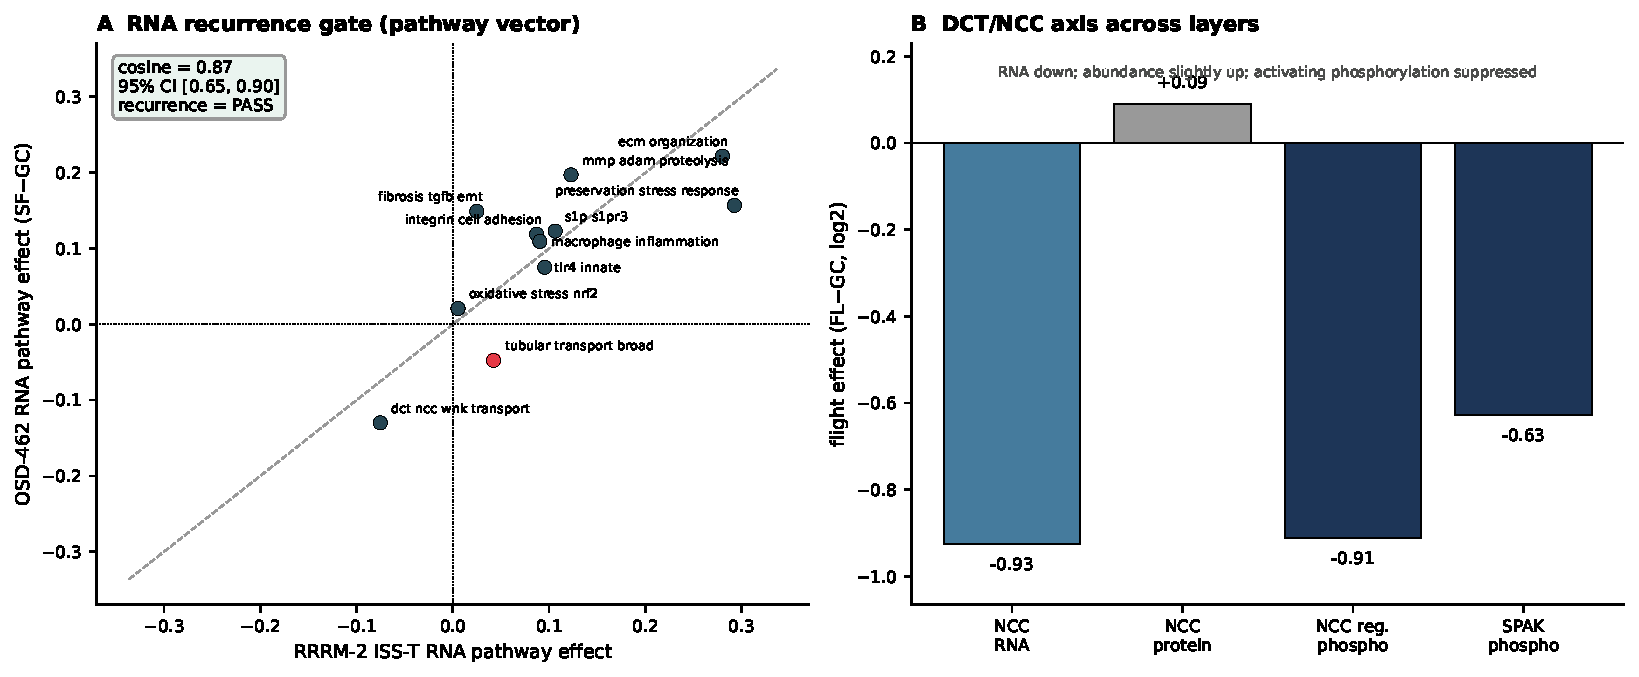
\includegraphics[width=0.92\textwidth]{fig_osd462_rna_recurrence.pdf}
\caption{\textbf{OSD-462 RNA recurrence gate.} The OSD-462 Space~Flight minus Ground~Control RNA pathway vector reproduces the RRRM-2 ISS-T matrix-high / DCT-low direction (cosine $0.87$, 95\% CI $0.65$--$0.90$). Leave-one-pathway-out diagnostics show the recurrence does not depend on any single pathway.}
\label{fig:osd462rna}
\end{figure}

\begin{figure}[H]
\centering
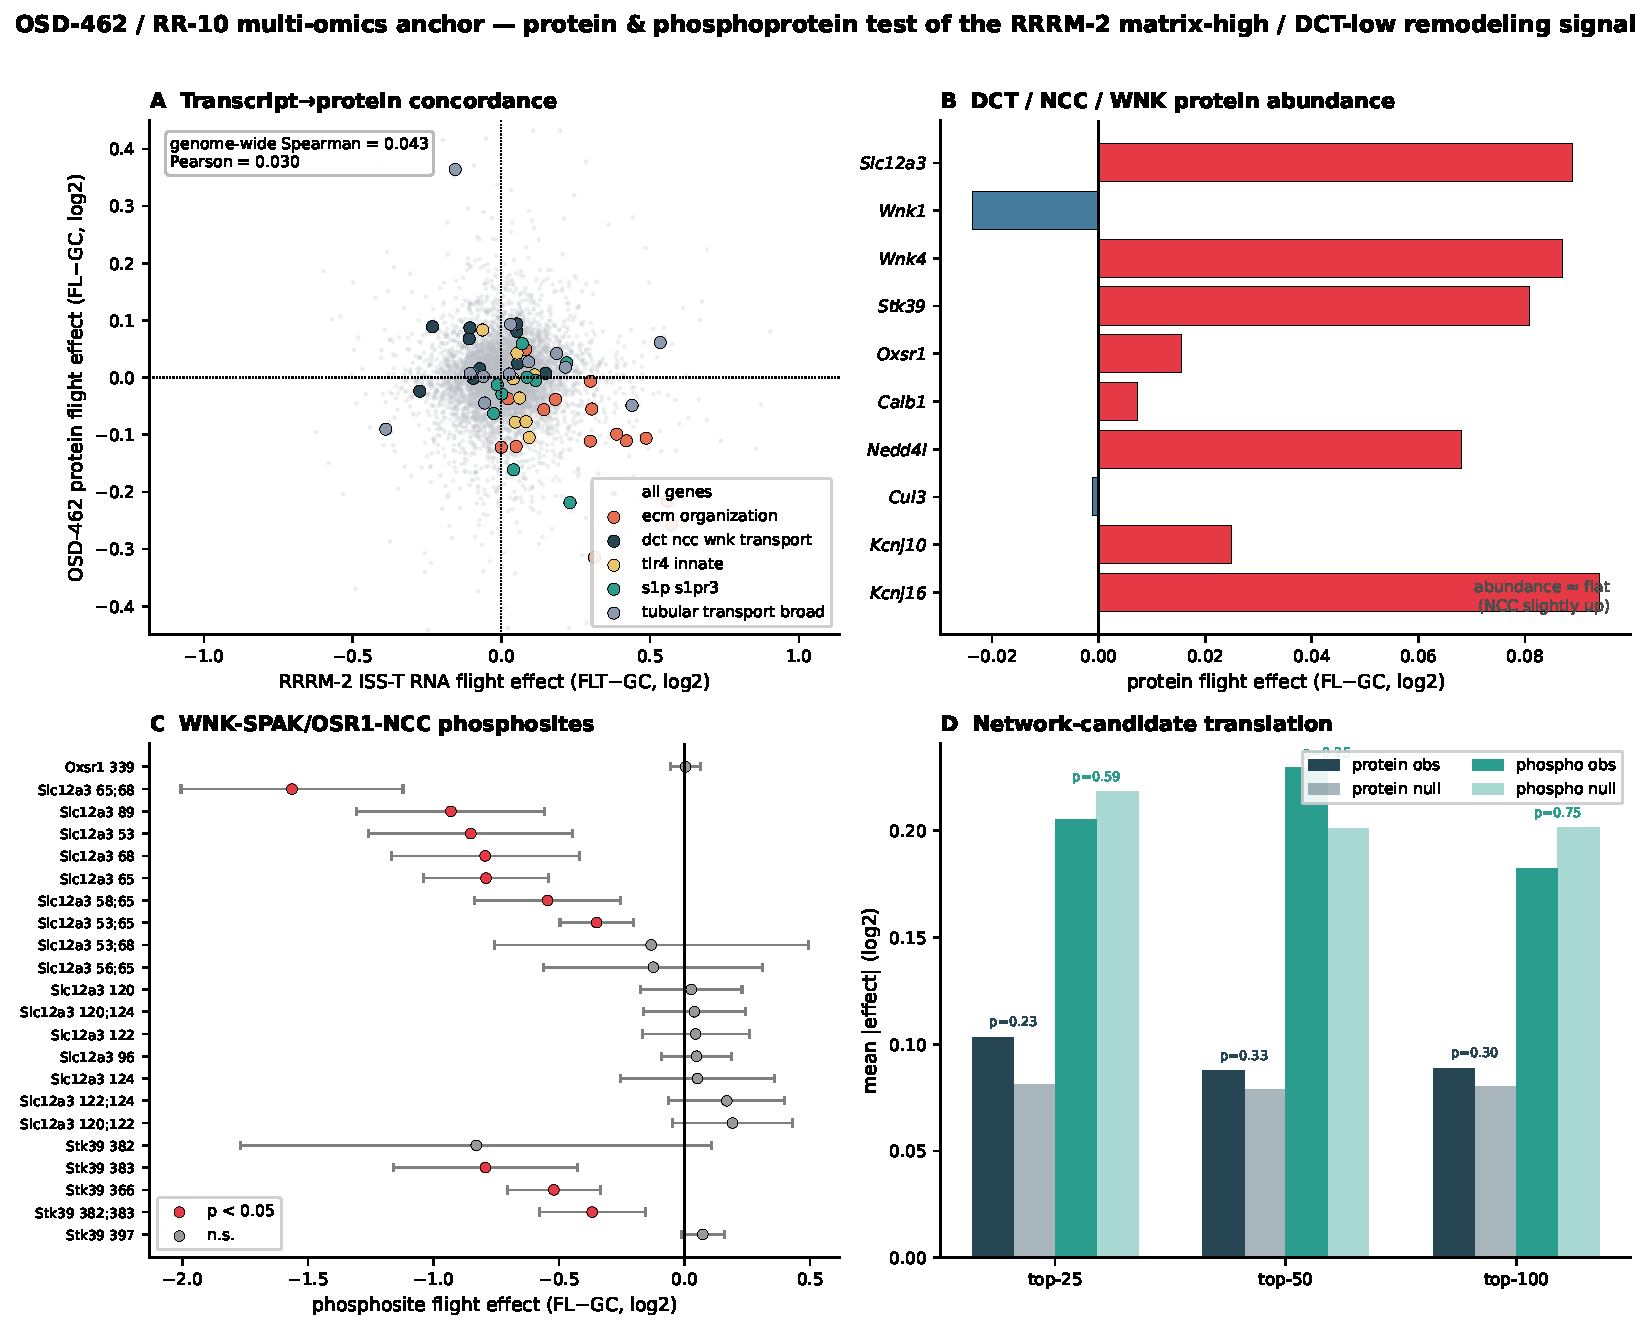
\includegraphics[width=\textwidth]{fig_osd462_multiomics_dashboard.pdf}
\caption{\textbf{OSD-462 multi-omic anchor dashboard.} Transcript-level recurrence with protein-abundance null and phospho-axis suppression. The WNK--SPAK/OSR1--NCC activating phosphosites are among the most strongly suppressed in the kidney phosphoproteome, while non-regulatory sites and total NCC protein are unchanged.}
\label{fig:osd462dash}
\end{figure}

Taken together, the anchor falsified protein-abundance concordance (H1, H2) and network translation (H4) and strongly supported phospho-axis suppression (H3). The transcriptomic matrix-high / DCT-low direction is reproducible across three cohorts, but its physical correlate is a change in NCC transport-pathway \emph{signaling activity}, not a change in transporter or matrix \emph{abundance} --- and that activity change is the same NCC dephosphorylation already documented in the Cosmic Kidney Disease study.

\subsection{KSEA confirms the Tier-1 phenotype: SPAK/OSR1 and WNK activity are inferred down}

Before linking the transcriptome to the phenotype anchor, the anchor itself was quantified as a regulator-activity endpoint. Kinase-substrate enrichment analysis applied to the OSD-462 phosphoproteome --- 21{,}083 quantified phosphosites forming the background distribution --- inferred that both kinases of the NCC-activating chain lose activity in flight (Table~\ref{tab:ksea}). SPAK/OSR1 activity was inferred down with $z=-6.31$ ($p=2.8\times10^{-10}$; mean substrate effect $-0.81$ log$_2$ units across three quantified substrate sites), and WNK activity was inferred down with $z=-4.12$ ($p=3.7\times10^{-5}$; mean substrate effect $-0.54$). Both passed the pre-specified positive-control rule, which required SPAK/OSR1 and WNK to return inferred activity down at $p<0.05$. This is not a new finding --- it is the expected consequence of the Cosmic Kidney Disease phenotype --- but its purpose is methodological: it confirms that the activity-inference layer is correctly implemented and sensitive, so that the regulator-activity machinery can be trusted when it is used for candidate nomination, and it expresses the Tier-1 anchor as a single interpretable activity score per kinase rather than as a scatter of individual sites.

\begin{table}[H]
\centering\small
\begin{tabular}{lrrrrl}
\toprule
Kinase & Substrate sites & Mean substrate effect & $z$ score & $p$ value & Inference \\
\midrule
SPAK/OSR1 & 3 & $-0.812$ & $-6.31$ & $2.8\times10^{-10}$ & activity down \\
WNK & 3 & $-0.539$ & $-4.12$ & $3.7\times10^{-5}$ & activity down \\
\bottomrule
\end{tabular}
\caption{\textbf{KSEA kinase-activity inference on the OSD-462 phosphoproteome.} Mean substrate effect is the mean Space~Flight minus Ground~Control log$_2$ phosphosite effect across quantified substrate sites; $z$ is standardized against all 21{,}083 quantified sites. Both kinases of the WNK--SPAK/OSR1--NCC chain pass the pre-specified positive-control rule (inferred activity down at $p<0.05$).}
\label{tab:ksea}
\end{table}

\subsection{Cross-cohort regulator activity recovers expected injury programs but no non-obvious driver}

With the activity-inference machinery certified by the KSEA positive control, transcription-factor and pathway activity were inferred from RNA within each of five cohorts to search for a non-obvious upstream organizer of the remodeling axis (Figure~\ref{fig:sixrecms}D). Across the four terminal-flight cohorts the recurrently-activated pathways are the programs already expected from kidney injury --- NF-$\kappa$B, TNF$\alpha$, JAK-STAT, and hypoxia --- and every one of them reverses sign in the RRRM-2 \LAR{} live-return arm, the directional behavior expected if they index an active terminal-flight injury state that recovers after return. Of 751 transcription factors scored in all four cohorts, none recur as inferred \emph{down}, and no single non-obvious factor dominates. The most coherent non-obvious recurrent signal is an endothelial/vascular transcription-factor module (\gene{Erg}, \gene{Gata2}, \gene{Ets1}), with the macrophage factor \gene{Spi1} and the retinoid receptors \gene{Rara}/\gene{Rarg} also recurrent; the endothelial module is biologically consistent with the S1P/S1PR3 and adhesion components of the RNA neighborhood. The honest verdict is therefore claim discipline: regulator-activity inference does not nominate a robust non-obvious driver beyond known injury and stress-response pathways, and the endothelial/vascular axis is reported as a candidate context axis rather than a proven regulator.

\subsection{Phenotype anchoring: the DCT transport RNA program co-varies with measured NCC activity}

The decisive test of the evidence ladder is the animal-matched comparison between the DCT transport RNA program and the measured NCC regulatory-phosphorylation activity, on the 20 Space~Flight and Ground~Control RR-10 animals that carry both modalities (Table~\ref{tab:phenoanchor}).

At the \emph{group level} the two scores are concordant. Flight lowers the DCT transport RNA program ($-0.32$) and lowers NCC regulatory phosphorylation ($-1.30$); the group effects share sign, as a genuine phenotype-coupled signal should. The specificity of this group effect is visible in the controls: the regulatory phosphosite cluster is suppressed about 4.3 times more strongly than the non-regulatory NCC phosphosites ($-1.30$ versus $-0.30$), and the RNA-side group effect survives removal of the \gene{Slc12a3} transcript from the score ($-0.25$). Group-level concordance between the transcriptomic DCT transport program and the measured NCC regulatory phosphorylation is therefore supported, and supported specifically at the regulatory sites.

At the \emph{per-animal level} the link is positive but underpowered. The all-sample Spearman correlation between the RNA score and the NCC regulatory-activity score is $+0.33$ ($p=0.16$); the condition-adjusted correlation, which removes the group means and is the real test of an animal-level link, is $+0.37$ ($p=0.11$). The sensitivity variant that adds \gene{Slc12a3} Thr89 gives $+0.34$ / $+0.32$, and the \gene{Slc12a3}-removed RNA score gives $+0.30$ / $+0.36$ --- all positive, none significant. This is exactly the underpowered-at-$n=20$ outcome anticipated in the Methods: a consistent positive direction without the precision to certify it. The interpretation label returned by the pre-specified rule is \emph{group-level concordant, animal-level underpowered}.

One control behaves in a way that must be reported openly. The non-regulatory NCC phosphosites, intended as a negative control, also correlate per-animal with the DCT transport RNA score, and more strongly than the regulatory sites ($+0.55$, $p=0.011$ all-sample; $+0.47$, $p=0.035$ condition-adjusted). The per-animal covariation is therefore \emph{not} exclusive to regulatory sites: the most plausible reading is that all NCC phosphosites partly track per-animal DCT-cell content or total NCC abundance, so per-animal correlation alone cannot establish regulatory-site specificity. The specificity evidence in this analysis is consequently the \emph{group-level magnitude} difference --- regulatory sites suppressed $\sim$4$\times$ more than non-regulatory sites --- and not the per-animal correlation. This wrinkle is reported rather than hidden, and it sets the honest claim ceiling: group-level concordance between the DCT transport RNA program and measured NCC regulatory phosphorylation is supported; an animal-level predictive link is suggestive but underpowered.

\begin{table}[H]
\centering\small
\resizebox{\textwidth}{!}{%
\begin{tabular}{lrrrrrrl}
\toprule
Comparison & $n$ & Group RNA & Group phospho & Spearman & $p$ & Spearman & $p$ \\
 & animals & FLT$-$GC & FLT$-$GC & all-sample & all & cond.-adj. & cond.-adj. \\
\midrule
Regulatory sites vs RNA & 20 & $-0.324$ & $-1.298$ & $+0.328$ & 0.158 & $+0.365$ & 0.113 \\
\quad + Slc12a3 Thr89 (sensitivity) & 20 & $-0.324$ & $-1.299$ & $+0.343$ & 0.139 & $+0.325$ & 0.162 \\
Non-regulatory sites vs RNA (control) & 20 & $-0.324$ & $-0.299$ & $+0.555$ & 0.011 & $+0.474$ & 0.035 \\
Regulatory vs RNA, Slc12a3 removed (control) & 20 & $-0.247$ & $-1.298$ & $+0.301$ & 0.198 & $+0.364$ & 0.115 \\
\bottomrule
\end{tabular}
}
\caption{\textbf{Animal-matched phenotype-anchoring comparison within OSD-462 / RR-10.} Per-animal DCT transport RNA score versus per-animal NCC phosphorylation activity score, on 20 Space~Flight and Ground~Control animals carrying both modalities. Group effects are concordant (same sign) for the regulatory comparison; the regulatory phosphosite cluster is suppressed $\sim$4.3$\times$ more than non-regulatory sites. Per-animal correlations are positive throughout but non-significant. The non-regulatory-site control also correlates per-animal, so per-animal specificity cannot be claimed; the specificity evidence is the group-level magnitude difference.}
\label{tab:phenoanchor}
\end{table}

\subsection{Marker-panel decomposition localizes part of the DCT-low signal to interstitial expansion}

Because the DCT-low signal is read from bulk tissue, a curated marker-panel decomposition was used to ask whether it reflects transcriptional suppression within DCT cells or a change in tissue composition (Figure~\ref{fig:sixrecms}E). Across the four flight cohorts, the DCT \emph{transport} program and the DCT \emph{identity} panel fall \emph{together} (OSD-462 identity $-1.00$, OSD-513 $-1.48$, OSD-253 $-1.59$), while the endothelial and stromal/fibroblast compartments rise recurrently. Within OSD-462 the largest per-sample flight increases are the endothelial ($+1.00$, $p=0.036$) and stromal ($+0.67$, $p=0.054$) scores, and per animal the endothelial compartment score \emph{anti-correlates} with the measured NCC regulatory-phosphorylation score ($\rho=-0.76$, $p=0.0004$; stromal $\rho=-0.51$, $p=0.023$), whereas the DCT identity score tracks it positively ($\rho=+0.52$, $p=0.020$). Because DCT identity falls alongside transport while interstitial compartments expand, the bulk DCT-low signal carries a genuine composition / interstitial-expansion component and cannot be read as pure cell-autonomous transcriptional suppression. This bounds the ``state'' language and, importantly, reinforces why the regulatory-phosphosite layer --- normalized within the phosphoproteome and suppressed $\sim$4$\times$ more at regulatory than non-regulatory sites --- is the more reliable transporter readout than bulk RNA: the phosphosite specificity is exactly what a composition shift cannot produce.

\begin{figure}[H]
\centering
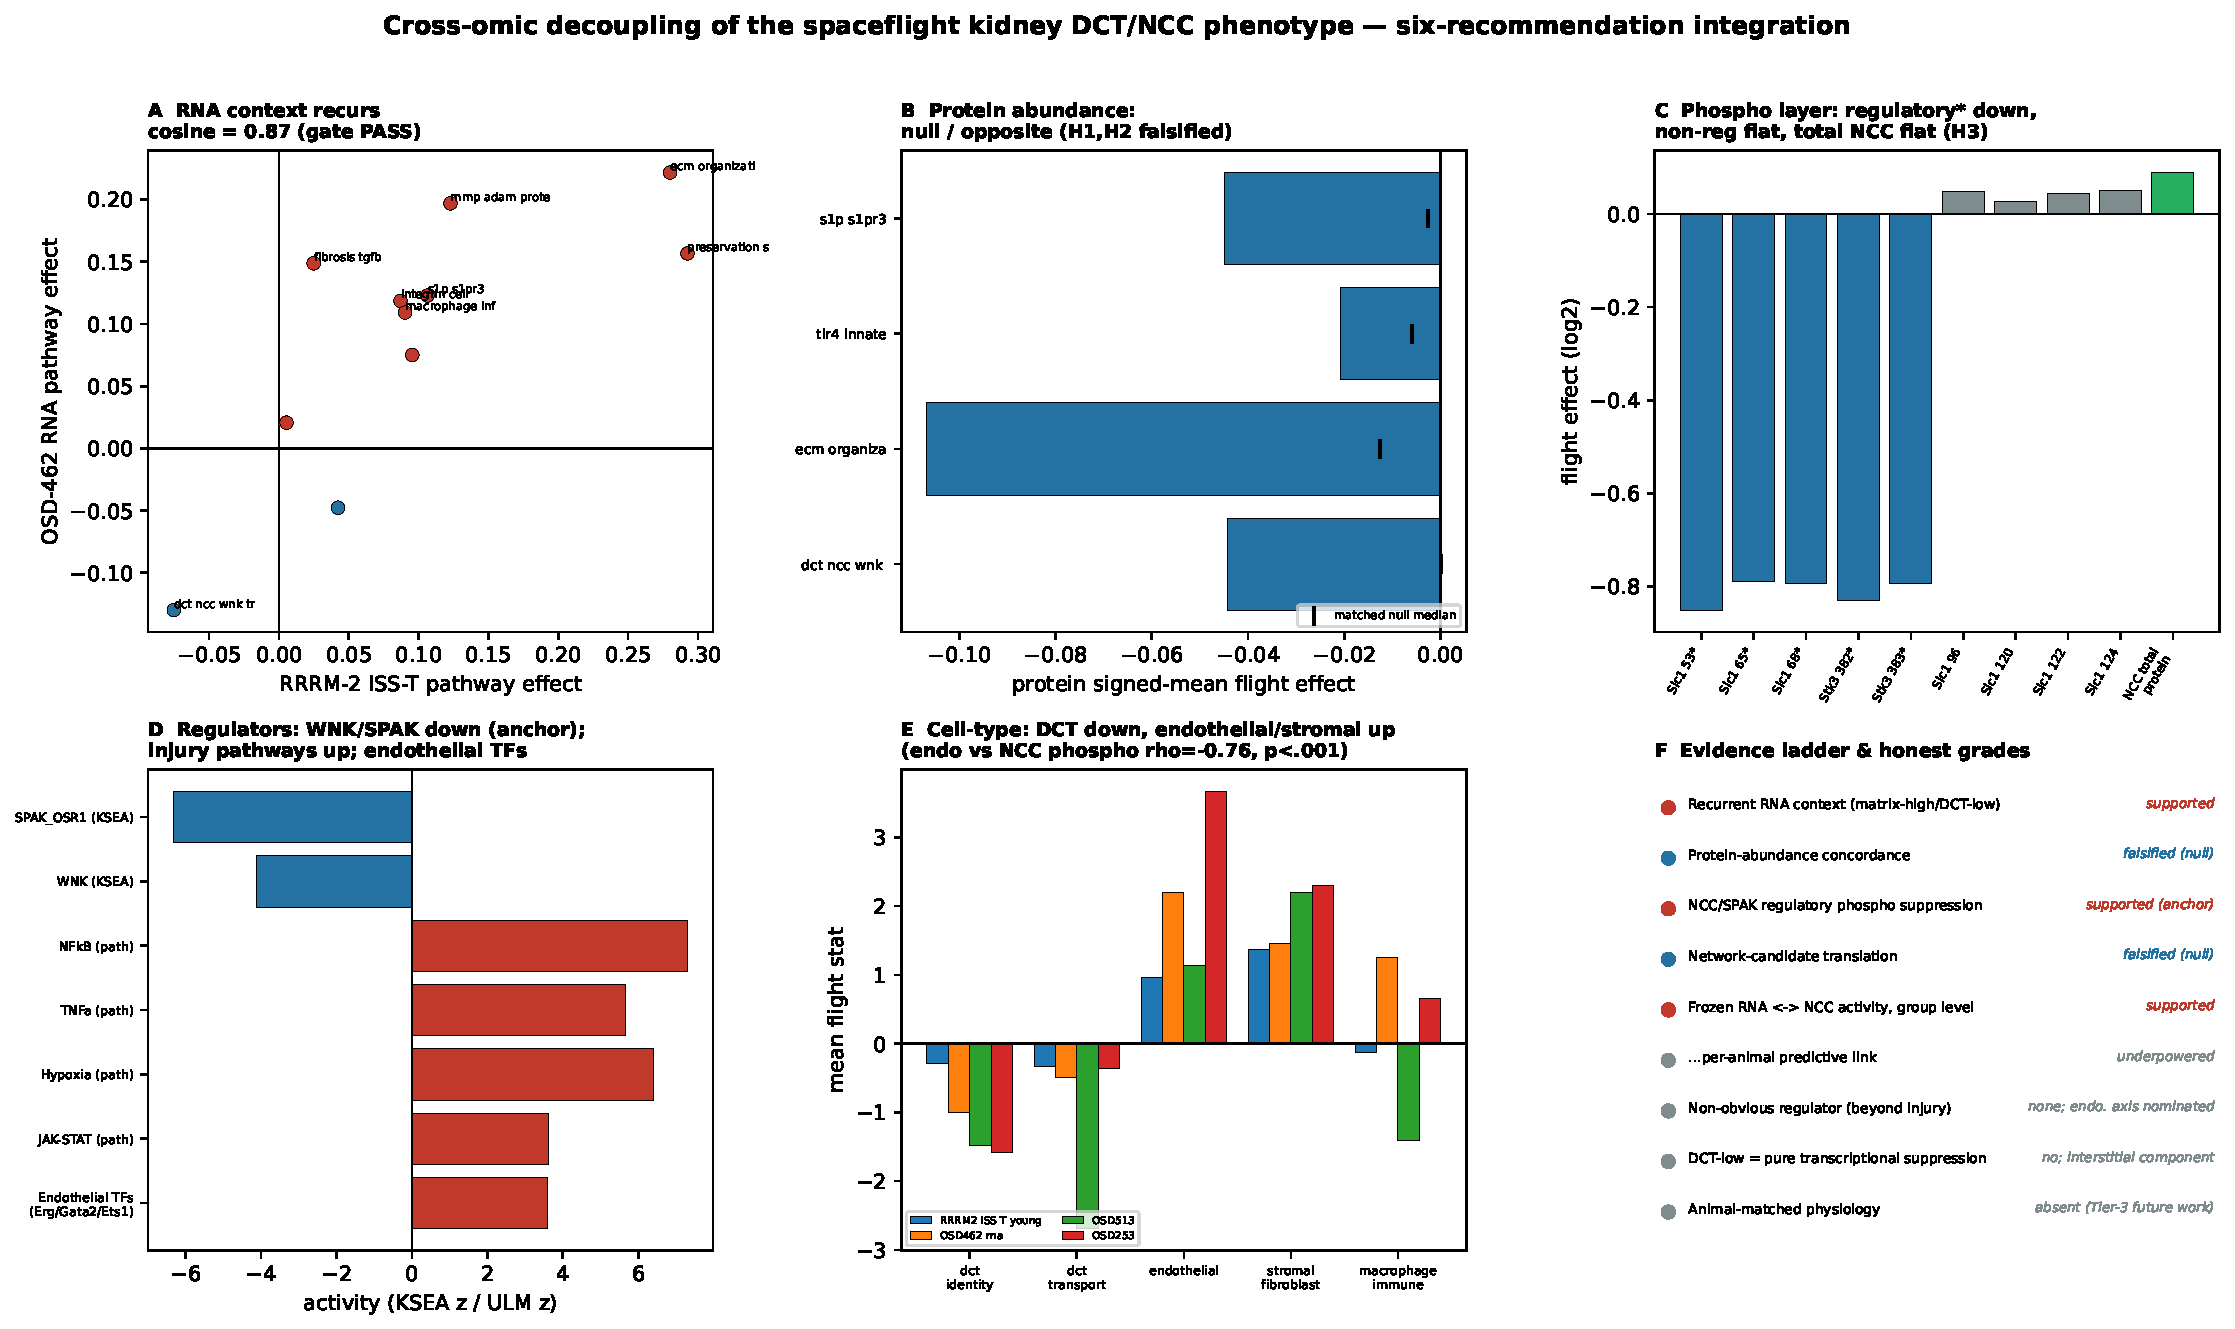
\includegraphics[width=\textwidth]{fig_sixrec_integration.pdf}
\caption{\textbf{Consolidated cross-omic decoupling of the spaceflight kidney DCT/NCC phenotype.} (A)~The matrix-high/DCT-low RNA pathway vector recurs between RRRM-2 \ISS{} and OSD-462 (cosine $0.87$, recurrence gate PASS). (B)~Matched-null protein-abundance concordance is null or opposite for both matrix (ECM) and DCT families (H1, H2 falsified). (C)~On the WNK--SPAK/OSR1--NCC chain, activating regulatory phosphosites (asterisk) are strongly suppressed while non-regulatory \gene{Slc12a3} sites and total NCC protein are flat (H3 supported). (D)~KSEA returns WNK and SPAK/OSR1 inferred-activity down (anchor); decoupler recurrent pathway activity is dominated by expected injury programs, with an endothelial/vascular transcription-factor module as the most coherent non-obvious recurrent signal. (E)~Marker-panel decomposition: DCT identity \emph{and} transport fall while endothelial/stromal compartments rise across cohorts; per animal the endothelial score anti-correlates with NCC regulatory phospho ($\rho=-0.76$, $p<0.001$). (F)~Evidence ladder and honest grades.}
\label{fig:sixrecms}
\end{figure}

\subsection{Claim hierarchy emerging from the full analysis}

The final claim hierarchy is:
\begin{enumerate}
  \item RRRM-2 does not resolve the planned within-cohort age-dependent rewiring contrast at primary module/pathway scale.
  \item RRRM-2 ISS-T aligns with an independent OSD-513 kidney flight direction; RRRM-2 LAR directionally anti-aligns but does not pass the external-label permutation null.
  \item The aligned ISS-T direction is a matrix-high / DCT-low tubulointerstitial state.
  \item LAR shows no detectable pooled matrix-minus-DCT flight response, so the primary LAR interpretation is attenuation relative to ISS-T. The young-LAR opposite point estimate is hypothesis-generating because the LAR effect itself is not significant and the state-space bootstrap CI crosses zero.
  \item Mechanism-score vectors support LAR divergence from ISS-T. Matrix/S1P/innate, clock-DCT, and tubular-transport projections are retained as follow-up mechanism hypotheses, not as confirmed separable programs.
  \item OSD-253 suggests TLR4/innate association, while the C3H/HeJ comparison favors a broader remodeling program rather than strict TLR4 requirement.
  \item The matrix-high / DCT-low RNA direction reproduces in a third independent cohort: the OSD-462 (RR-10) RNA flight effect recurs the RRRM-2 ISS-T direction (pathway-vector cosine $0.87$, 95\% CI $0.65$--$0.90$).
  \item In OSD-462, the RNA direction does not translate to protein abundance --- targeted protein concordance is null, matrix proteins move opposite their transcripts, and total NCC protein is unchanged.
  \item The OSD-462 phosphoproteome localizes the signal to transport-pathway activity: the WNK--SPAK/OSR1--NCC activating phosphorylation cluster is specifically suppressed, with non-regulatory sites unchanged. This independently reproduces the Cosmic Kidney Disease NCC dephosphorylation phenotype \citep{siew2024cosmic}.
  \item KSEA applied to the OSD-462 phosphoproteome infers SPAK/OSR1 ($z=-6.31$) and WNK ($z=-4.12$) activity down, passing the pre-specified positive-control rule and quantifying the Tier-1 phenotype as a regulator-activity endpoint.
  \item Cross-cohort transcription-factor and pathway-activity inference (decoupler, five cohorts) recovers the expected injury programs (NF-$\kappa$B, TNF$\alpha$, JAK-STAT, hypoxia; all reversing in \LAR) but nominates no robust non-obvious upstream driver; the most coherent non-obvious recurrent signal is an endothelial/vascular transcription-factor module (\gene{Erg}, \gene{Gata2}, \gene{Ets1}), reported as a candidate context axis.
  \item Animal-matched within RR-10 ($n=20$), the DCT transport RNA program and measured NCC regulatory phosphorylation are concordant at group level (both lowered in flight; regulatory cluster suppressed $\sim$4.3$\times$ more than non-regulatory sites). The per-animal link is positive but underpowered (Spearman $+0.33$ to $+0.37$, $p\approx0.11$--$0.16$). A non-regulatory-site control also co-varies per-animal, so per-animal specificity is not claimed; the supported claim is group-level concordance plus a suggestive, underpowered animal-level link.
  \item Marker-panel decomposition shows the bulk DCT-low signal includes an interstitial-expansion/composition component --- DCT identity and transport markers fall together while endothelial and stromal compartments rise, and the per-animal endothelial score anti-correlates with measured NCC phosphorylation ($\rho=-0.76$) --- so it is not pure DCT transcriptional suppression, which reinforces the phosphosite layer as the more reliable transporter readout.
  \item WGCNA, LIONESS, and node2vec provide structural annotation and exploratory gene prioritization below the cross-cohort pathway/module and mechanism-state results; their candidate genes show no independent protein- or phosphoprotein-level support in OSD-462, which is reported as a negative result on the added value of network methods.
\end{enumerate}

% =====================================================================
\section{Discussion}

\subsection{Principal biological interpretation}

The central result of this study is not that a matrix-high / DCT-low remodeling context exists --- matrix activation and distal-transport suppression are individually expected from kidney injury biology. The result is how that context behaves \emph{across omic layers}. Across RRRM-2 ISS-T, OSD-513, and OSD-462 RNA, flight is associated with a coordinated and recurrent matrix-high / DCT-low transcriptomic context: extracellular-matrix organization, cell adhesion, proteolysis, innate/stress-associated biology, and S1P/S1PR3-related features rise, while distal convoluted tubule transport programs fall. But in the one cohort with matched proteomics and phosphoproteomics, that recurrent RNA context does not propagate as a protein-abundance change; it resolves at the regulatory-phosphorylation layer. Spaceflight kidney remodeling is, in this specific and testable sense, \emph{cross-omically decoupled}. That decoupling --- not the RNA context by itself --- is the strongest and most transferable object recovered by the analysis, and it is the spine of the interpretation that follows.

This interpretation reframes the project away from a broad age-rewiring model. RRRM-2 was initially attractive because its factorial design could, in principle, ask whether spaceflight amplifies, dampens, or redirects age-associated kidney networks. In practice, the within-cohort control-aging directions were too unstable at primary module/pathway resolution to support that claim. The more defensible biology is a flight-associated tubulointerstitial remodeling context that recurs across independent kidney spaceflight cohorts, is modulated by live return, and --- crucially --- is expressed at the activity layer rather than the abundance layer.

\subsection{Relationship to the Cosmic Kidney Disease study}

The most important context for interpreting this work is the Cosmic Kidney Disease study \citep{siew2024cosmic}, which characterized spaceflight-induced renal dysfunction across mice, rats, and astronauts with integrated transcriptomic, proteomic, phosphoproteomic, physiological, and morphological data, and reported NCC and distal nephron transporter dephosphorylation together with distal convoluted tubule remodeling. The mouse kidney phosphoproteomics in that study is the RR-10 experiment, deposited as OSD-462 and used here as the multi-omic anchor. The present analysis therefore does not claim to discover that spaceflight dephosphorylates NCC or that the distal convoluted tubule remodels; that phenotype is established.

What this work adds is not the phenotype but its \emph{context} and its \emph{cross-omic behavior}. The Cosmic Kidney Disease study centered the transporter lesion; it did not ask whether that lesion is an isolated distal-tubule event or part of a reproducible kidney-wide remodeling context, nor at which omic layer that context is expressed. This work answers both. First, the matrix-high / DCT-low context recurs across RRRM-2 (OSD-771) and OSD-513 --- cohorts not part of the Cosmic Kidney Disease study --- and again in OSD-462 RNA, establishing it as a reproducible cross-cohort feature rather than a single-study result. Second, anchoring that context to the matched OSD-462 protein and phosphoprotein layers shows it is cross-omically decoupled: it does not appear as matrix- or transporter-protein abundance change, and the measurable transporter lesion is post-translational. The honest statement of novelty is therefore precise: this is not a discovery of NCC dephosphorylation, and it is not merely a reproduction of it; the contribution is a reproducible cross-omic context map that shows \emph{where} --- in cohorts and in omic layers --- the established phenotype does and does not generalize, together with the methodological lesson that bulk-RNA recurrence must not be over-read as protein-level change.

\subsection{The phenotype anchor and the evidence ladder}

The methodological core of this work is that the analysis is hung off a measured endpoint rather than off a moved pathway score. This matters because the most common failure mode of high-dimensional spaceflight transcriptomics is to mistake a statistically moved construct for a biological phenotype. By fixing the anchor as the measured suppression of NCC/SPAK regulatory phosphorylation --- an endpoint that is independently established by the Cosmic Kidney Disease study \citep{siew2024cosmic} and is mechanistically specific within the WNK--SPAK/OSR1--NCC chain --- every transcriptomic claim in the paper can be graded by how directly it connects to that anchor.

The KSEA layer is the first payoff of that discipline. Rather than asserting that the phosphosite table ``shows'' kinase suppression, KSEA expresses it as a single standardized activity score per kinase and submits it to a pre-specified positive-control rule. That SPAK/OSR1 ($z=-6.31$) and WNK ($z=-4.12$) both pass is unsurprising biologically but valuable methodologically: it certifies that the regulator-activity machinery is sensitive and correctly implemented, which is the precondition for trusting the same machinery when it nominates candidate transcription factors and pathways. A positive control that passes is not a discovery; it is a license to use the tool.

The animal-matched comparison is the rung of the ladder that the available data can actually test, and its result is deliberately reported with a confidence label rather than a headline. Group-level concordance is real and specific: flight lowers both the DCT transport RNA program and measured NCC regulatory phosphorylation, and the regulatory phosphosites are suppressed roughly fourfold more than non-regulatory sites, which is the magnitude signature expected if the regulatory cluster is the genuinely targeted feature. The per-animal link is positive across every variant and control, but it does not reach significance at twenty animals, and the condition-adjusted test --- the honest test of an animal-level link once group means are removed --- is likewise non-significant. The most important piece of intellectual honesty in the paper is the non-regulatory-site control: it was meant to be a clean negative, and it was not, because non-regulatory NCC phosphosites also co-vary per-animal with the RNA score. The reasonable interpretation is that per-animal NCC phosphosite intensity partly tracks DCT-cell content or total NCC abundance, so per-animal correlation cannot by itself establish regulatory-site specificity. Reporting this openly, and relocating the specificity claim to the group-level magnitude difference where it is genuinely supported, is the correct response. The honest claim ceiling is therefore precise: group-level concordance between the DCT transport RNA program and measured NCC regulatory phosphorylation is supported; an animal-level predictive link is suggestive but underpowered.

Stated as a ladder, the evidence is: RNA-state recurrence across cohorts (supported); measured NCC/SPAK regulatory-phosphorylation suppression as the Tier-1 anchor, quantified by targeted phosphosite effects and by KSEA (supported, and reproduced from Cosmic Kidney Disease rather than discovered); group-level coupling of the transcriptomic DCT program to that measured anchor (supported); an animal-level predictive link (suggestive, underpowered); DCT morphological remodeling as a Tier-2 literature anchor (taken from Cosmic Kidney Disease, not measured here --- in that study's source data, spaceflight reduces DCT NCC-positive tubule density by $\sim$48\% ($p=0.001$), a morphological correlate consistent with the measured phospho suppression); and physiology --- urine and serum electrolytes, blood pressure --- as a Tier-3 rung that these datasets cannot reach and that is named explicitly as future work, since no animal-level physiology is present in the OSD-462 omics record. The contribution is the honest construction and labelling of this ladder, not the conquest of its top rung.

\subsection{Cross-omic decoupling as the central result}

The defining result of the multi-omic anchor, and the thesis of this paper, is a dissociation between omic layers. The transcriptomic remodeling context reproduced cleanly at the RNA level, yet pre-registered protein-abundance concordance was null for every targeted gene set, matrix proteins moved opposite their transcripts, and total NCC protein abundance did not change. The signal that did move was phosphorylation: the SPAK/OSR1-target activating cluster on NCC was strongly and specifically suppressed, and KSEA independently inferred WNK and SPAK/OSR1 activity loss. Had the matrix-high / DCT-low recurrence reflected simple abundance remodeling, matrix proteins would have risen and transporter proteins would have fallen; neither happened. The biological reading is that the spaceflight kidney transcriptomic remodeling context corresponds to a change in transport-pathway \emph{signaling activity} rather than to bulk changes in transporter or matrix protein abundance --- the recurrent RNA context is best understood as a kidney-wide setting for a phosphorylation-layer transporter phenotype, not as a direct protein-abundance signature.

This cross-omic decoupling carries a direct and transferable methodological consequence for spaceflight transcriptomics, where bulk RNA-seq is often the only modality available: an RNA-level ``DCT transport down'' signature should be interpreted as a candidate activity/regulation change to be confirmed at the phosphoprotein layer, not as evidence that transporter protein is lost; and an RNA-level matrix-up signature should not be read as matrix-protein deposition. The matrix-protein result --- transcripts up, soluble proteins modestly down --- should itself be read cautiously, because bulk proteomics with sum-to-100 normalization can show compositional effects and because secreted matrix proteins may partition out of the soluble proteome; it is reported as an observation, not a mechanism. The cell-type decomposition (below) gives the decoupling a concrete cause: because the bulk DCT-low signal partly reflects interstitial expansion rather than cell-autonomous transcriptional change, the phosphoproteome --- normalized within itself and specific to regulatory sites --- is the layer at which the transporter phenotype is least confounded.

\subsection{What network methods did and did not contribute}

A frank assessment of the network layer is warranted because network rewiring was the original motivation for the project. WGCNA provided interpretable module structure, and LIONESS/node2vec nominated candidate genes. But when those network-prioritized candidates were tested for independent support in the OSD-462 proteome and phosphoproteome, they showed no enrichment. The network layer did not translate to protein-level biology. This is reported as a negative result rather than omitted. The practical lesson, consistent with the statistical fragility of small-cohort co-expression and embedding metrics, is that sample-specific network and embedding methods at $n=5$ per cell are best treated as hypothesis-generating annotation, and that pathway-scale contrasts with external recurrence and orthogonal-omic anchoring carried essentially all of the defensible signal in this study.

\subsection{A tubulointerstitial remodeling state}

The word remodeling is used deliberately. The transcriptomic pattern is not simply generic differential expression, and it is not by itself proof of established fibrosis. It is a tissue-state signal in which matrix, adhesion, proteolysis, innate immune context, and tubular transport move together. In kidney biology, these processes are plausibly linked: renal injury and repair programs commonly involve epithelial stress, inflammatory signaling, fibroblast and matrix activation, altered cell-matrix adhesion, and changes in segment-specific transport identity \citep{liu2011fibrosis,natneph2024fibrosis,jci2024fibrosis,chavula2022cadherin}. The present data place the spaceflight-associated kidney response in that injury-repair/remodeling neighborhood.

The distal tubule side of the axis is especially important. DCT/NCC-WNK biology is not only a marker panel; it represents a physiologic transport system involved in sodium-chloride handling, potassium-sensitive WNK-SPAK/OSR1 signaling, and downstream electrolyte and blood-pressure regulation \citep{castaneda2024dct,ge2016wnk}. Suppression of this program alongside ECM/adhesion/proteolysis activity suggests a kidney state in which specialized distal nephron transport identity is reduced while matrix and interstitial remodeling programs are engaged. That coupling is the main biological signal in the study.

This does not mean that transcriptomics has measured fibrosis, transport function, or renal injury directly. The appropriate conclusion is more constrained: terminal-flight kidney transcriptomes carry molecular evidence for a matrix-remodeling/high-stress state coupled to lower distal-nephron transport signatures. The result nominates concrete tissue and physiology endpoints for validation, including collagen deposition, tubular injury markers, immune infiltration, vascular/interstitial markers, urine and serum chemistry, and segment-specific NCC/WNK abundance or phosphorylation. A marker-panel decomposition further qualifies the distal-tubule side: DCT identity and transport markers fall \emph{together} while endothelial and stromal compartments expand, and the per-animal endothelial score anti-correlates with measured NCC phosphorylation ($\rho=-0.76$). Part of the bulk DCT-low signal is therefore attributable to interstitial expansion or changing segment composition rather than to purely cell-autonomous transcriptional suppression --- an additional reason the phosphorylation-activity layer, not bulk RNA, is treated as the definitive transporter readout, since regulatory-site phosphosite specificity is not something a composition shift can manufacture.

\subsection{What live return changes}

The live animal return arm is biologically informative because it does not simply preserve the terminal-flight state. At the pooled scalar level, LAR shows no detectable matrix-minus-DCT state shift, whereas ISS-T shows a clear positive shift. This supports attenuation of the terminal-flight remodeling state after return rather than a confirmed reversal. The age-stratified young-LAR opposite point estimate remains hypothesis-generating because the LAR effect is not statistically distinguishable from zero.

The more interesting LAR interpretation is decoupling. Matrix/S1P/innate features and \gene{S1pr3} show strong arm divergence, with ISS-T-positive and LAR-negative behavior. DCT transport features, however, do not show a clean pooled recovery. Thus, return may reduce or redirect the matrix/innate/S1P arm of the terminal-flight response while leaving distal transport biology incompletely recovered, weakly affected, or differently organized. In biological terms, the data are more consistent with a transition between an active terminal-flight injury-repair state and a post-return recovery/reloading state than with a simple ``flight effect disappears'' model.

Clock-associated DCT features add a plausible but limited recovery-context signal. \gene{Per2} and clock-score behavior separate ISS-T from LAR and correlate with the DCT/state components. Because RRRM-2 is not a time-course experiment and time-of-day information is insufficient for phase inference, this should be described as a clock-gene-associated transcriptional state, not as evidence of circadian phase shifting.

\subsection{Mechanistic neighborhood}

The mechanism-score results place the remodeling state near ECM organization, adhesion/proteolysis, TLR4/innate signaling, macrophage/inflammatory context, S1P/S1PR3 biology, and DCT/NCC-WNK suppression. This is a plausible renal injury-remodeling neighborhood. TLR4 and innate immune signaling can promote inflammatory and fibrotic kidney injury, TRIL is connected to TLR3/TLR4 signaling, integrins and cadherins participate in cell-matrix and fibroblast-like adhesion, MMP/ADAM proteases mediate matrix turnover, and S1P/S1PR3 signaling has recognized links to vascular, immune, inflammatory, and fibrotic responses \citep{souza2015tlr4,carpenter2009tril,carpenter2011tril,wochal2014tril,s1p2017,s1p2020,s1p2009}.

OSD-253 helps set a boundary around this interpretation. If the state were strictly TLR4-dependent, it should collapse in the TLR4-impaired C3H/HeJ context. Instead, the remodeling score is lower in C3H/HeJ at the point-estimate level, but strain-delta confidence intervals cross zero, and ECM/fibrosis/adhesion/proteolysis scores remain positive in C3H/HeJ under the white-LED rerun control scenario. The safer conclusion is that TLR4/innate biology is associated with, and may amplify or contextualize, the remodeling state; it is not established as a required single upstream driver.

\subsection{Why this is not accelerated kidney aging}

The negative aging result is important. Projection onto an external Tabula Muris Senis kidney aging axis did not support a simple accelerated-aging interpretation, and RRRM-2 control-aging vectors were too unstable to support the original age-rewiring claim. This does not make the analysis uninformative. It narrows the biology. The ISS-T signal is better described as flight-associated renal remodeling with distal transport suppression than as aged kidney mimicry. Age may still modify susceptibility or recovery, but the current design cannot make that interaction a primary claim.

\subsection{Role of WGCNA, LIONESS, and node2vec}

The network methods are best understood as annotation and prioritization layers below the pathway/state result. WGCNA maps the remodeling state onto co-expression structure, especially an ECM/cell-migration module containing genes such as \gene{Tril}, \gene{Itga9}, \gene{Fbn1}, \gene{S1pr3}, \gene{Cdh11}, \gene{Adam12}, and \gene{Mmp14}. That module structure gives the pathway-level result a recognizable gene neighborhood.

LIONESS and node2vec answer a different, secondary question: which genes may have local network neighborhoods that move with the ISS-T remodeling program? The top-ranked genes include stress-response, metabolic, clock-associated, transport, and signaling candidates, including \gene{Rbm3}, \gene{Per2}, \gene{Cyp4a14}, and \gene{Bhmt}. These methods do not establish a separate gene-level topology-reversal claim. Their value is to nominate candidate genes and local neighborhoods for follow-up inside the broader remodeling/transport state.

\subsection{Limitations}

Several limitations constrain the interpretation. First, RRRM-2 has only $n=5$ per Age $\times$ Arm $\times$ Environment cell, limiting high-dimensional interaction estimation and making age-stratified LAR patterns descriptive. Second, ISS-T and LAR differ in flight state, return/recovery timing, reloading, and collection context; their contrast should not be interpreted as a pure recovery experiment. Third, the clock-DCT result cannot be interpreted as circadian phase because RRRM-2 is not a circadian time-course experiment. Fourth, external OSDR cohorts differ in sex, strain, mission, duration, sequencing, and metadata. Cross-cohort agreement at pathway-vector level is therefore meaningful, but raw expression pooling would be inappropriate. Fifth, OSD-253 has two imperfect control definitions, so it should remain a mechanism-context cohort rather than a clean validation endpoint. Sixth, curated mechanism signatures and bootstrap procedures cannot propagate every source of pipeline-level uncertainty. Seventh, the OSD-462 anchor is bulk whole-kidney proteomics and phosphoproteomics with a two-plex TMT design; although the NCC machinery was well quantified, bulk tissue dilutes distal convoluted tubule signal and TMT normalization can introduce compositional effects, which is one reason the matrix-protein result is treated as observational. Eighth, OSD-462 has no live-return arm and no aged animals, so it can corroborate only the ISS-T-side flight direction and cannot test the live-return or age-stratified observations. Ninth, and most importantly for framing, the spaceflight NCC dephosphorylation phenotype is not novel to this work: it was established by the Cosmic Kidney Disease study using the same RR-10 phosphoproteomics, and the present analysis reproduces rather than discovers it. Tenth, the animal-matched phenotype-anchoring comparison is underpowered: at twenty flight and ground animals the per-animal RNA$\leftrightarrow$activity correlation cannot be certified, and the non-regulatory-site control co-varies per-animal, so per-animal regulatory-site specificity cannot be claimed --- the supported claim is restricted to group-level concordance and the group-level magnitude difference. Eleventh, the KSEA layer uses a small, curated kinase-substrate network restricted to the WNK--SPAK/OSR1--NCC chain; it is a deliberate, individually cited positive control rather than a kinome-wide activity screen, and the supporting decoupler transcription-factor and pathway-activity layer yields ranked candidate lists that are explicitly suggestive and require independent validation. Twelfth, that cross-cohort regulator scan recovered the expected injury/inflammation programs but no robust non-obvious upstream driver, so the nominated endothelial/vascular axis is a candidate context axis only, and the marker-panel decomposition indicates the bulk DCT-low signal includes an interstitial-expansion/composition component, so it cannot be read as pure DCT transcriptional suppression. Thirteenth, no animal-level physiology (urine/serum electrolytes, blood pressure) exists in the OSD-462 record; the same-mission Cosmic Kidney Disease morphometry and electrolyte data provide only a group-level literature ladder, and animal-matched functional endpoints remain future work.

\subsection{Future work}

The most direct follow-up is tissue-level validation of the remodeling/transport axis. Collagen staining, tubular injury markers, immune and macrophage markers, vascular/interstitial markers, and segment-specific NCC/WNK assays would test whether the transcriptomic state corresponds to structural remodeling, tubular injury, or altered distal-nephron transport machinery. The LAR-specific question is whether return and reloading preferentially attenuate matrix/S1P/innate activity while leaving distal transport programs incompletely restored. A design powered for Age $\times$ Arm $\times$ Flight interaction would be needed before age-specific recovery or reversal can be claimed.

Mechanistically, TLR4-intact and TLR4-impaired comparisons should be paired with S1P/S1PR3, TGF-beta/ECM, adhesion/proteolysis, macrophage/innate, and DCT/WNK markers. Computationally, the next useful step is not to add more network machinery, but to preserve the claim hierarchy: cross-cohort pathway/state recurrence first, mechanism-context interpretation second, and network-neighborhood gene prioritization third.

% =====================================================================
\section{Conclusion}

This study is a cross-omic context-mapping analysis of the spaceflight kidney. Its thesis is that the established spaceflight DCT/NCC transporter phenotype is embedded in a recurrent kidney-wide RNA remodeling context, but that context is \emph{cross-omically decoupled}: it recurs in transcriptomes, fails as a simple protein-abundance story, and converges most clearly on NCC/SPAK phosphorylation-activity suppression. A matrix-high / DCT-low remodeling context recurs across three independent mouse kidney spaceflight cohorts (RRRM-2 ISS-T, OSD-513, and OSD-462 RNA), establishing it as a reproducible feature rather than a single-study artifact. Anchored against matched OSD-462 (RR-10) protein and phosphoprotein data under a pre-registered plan, the transcriptomic context does not correspond to transporter or matrix protein abundance; the measurable transporter lesion is the specific suppression of the WNK--SPAK/OSR1--NCC activating phosphorylation cluster, with KSEA independently confirming WNK and SPAK/OSR1 activity loss. A phosphoproteomics-naive RNA score and the measured NCC regulatory phosphorylation are concordant at group level but the per-animal link is underpowered at $n=20$; a cell-type decomposition shows the bulk DCT-low signal carries an interstitial-expansion component, which is itself why the phosphoproteome is the reliable transporter readout. A regulator-activity scan across five cohorts recovers expected injury programs but no non-obvious upstream driver, and co-expression network candidates do not translate to protein-level biology. RRRM-2 cannot support the original age-rewiring claim, and the live-return arm shows attenuation rather than reversal. The defensible value of the work is that it maps --- reproducibly, and omic layer by omic layer --- where a clinically relevant spaceflight transporter phenotype generalizes and where it does not, and supplies a concrete methodological warning that recurrent bulk-RNA remodeling must not be read as protein-level change.

\section*{Author contributions}
I.S. designed and implemented the analytical framework, conducted the contrast-vector, cross-OSDR, mechanism-axis, WGCNA-context, LIONESS/node2vec, multi-omic anchoring, KSEA regulator-activity, phenotype-anchoring, and sensitivity analyses, generated the figures, drafted the manuscript, and maintained the source code, tests, and run artifacts. Authorship and collaboration structure will be revised with mentor and collaborator input.

\section*{Competing interests}
The author declares no competing interests.

\section*{Data and code availability}
NASA Open Science Data Repository accessions: OSD-771 (RRRM-2), OSD-513, OSD-253, and OSD-462 (RR-10; the multi-omic anchor cohort, also the source of the Cosmic Kidney Disease mouse kidney phosphoproteomics). Tabula Muris Senis kidney was used as the external aging reference. Pipeline source, configuration files, run manifests, tests, figures, the pre-registered multi-omic analysis plan, and manuscript drafts are version-controlled in the project repository.

\begin{itemize}
  \item Main transcriptomic production run: \code{run\_20260519\_000547\_2500g}.
  \item Cross-OSDR permutation sensitivity run: \code{run\_20260519\_cosine\_perm\_null}.
  \item Primary mechanism-axis and tubulointerstitial state-space outputs: \path{data/results/run_20260519_000547_2500g/contrast_vectors/mechanism_axis}.
  \item Pre-registered OSD-462 multi-omic analysis plan: \path{docs/osd462_multiomics_analysis_plan.md}.
  \item OSD-462 multi-omic anchor run and outputs: \code{run\_20260521\_osd462\_anchor}; \path{data/results/run_20260521_osd462_anchor/osd462_anchor}.
  \item Multi-omic anchor module, layer scripts, and tests: \path{src/multiomics/osd462_anchor.py}; \path{scripts/osd462/}; \path{tests/test_osd462_anchor.py}.
  \item KSEA regulator-activity layer: module \path{src/multiomics/regulator_activity.py}; orchestrator \path{scripts/regulator_activity/run_regulator_activity.py}; curated kinase-substrate network \path{data/external/kinase_substrate/renal_kinase_substrate_core.tsv}; run \code{run\_20260522\_regulator\_activity}.
  \item Phenotype-anchoring layer: module \path{src/multiomics/phenotype_anchor.py}; orchestrator \path{scripts/regulator_activity/run_phenotype_anchor.py}; run \code{run\_20260522\_phenotype\_anchor} (\path{phenotype_anchor_summary.tsv}, \path{phenotype_anchor_per_animal.tsv}, \path{manifest.json}).
  \item Unit tests for the new layers: \path{tests/test_regulator_activity.py} and \path{tests/test_phenotype_anchor.py} (15 tests pass).
  \item Consolidated final-version plan: \path{docs/final_version_plan.md}.
  \item Methodology overview figure source: \path{latex_paper/figures_osd462/methodology_overview.tex}.
  \item 5,000-gene sensitivity run: \code{run\_20260519\_5000g\_sensitivity\_3seed}.
  \item Figure-generation scripts: \path{scripts/plot_manuscript_v4_figures.py}; \path{scripts/osd462/05_plot_dashboard.py}.
\end{itemize}

% =====================================================================
\begin{thebibliography}{99}\small

\bibitem{afshinnekoo2020fundamental} Afshinnekoo E, Scott RT, MacKay MJ, et al. Fundamental biological features of spaceflight: advancing the field to enable deep-space exploration. \emph{Cell}. 2020;183:1162--1184. doi:10.1016/j.cell.2020.10.050.

\bibitem{badia2022decoupler} Badia-i-Mompel P, V\'elez Santiago J, Braunger J, et al. decoupleR: ensemble of computational methods to infer biological activities from omics data. \emph{Bioinformatics Advances}. 2022;2:vbac016. doi:10.1093/bioadv/vbac016.

\bibitem{benjamini1995controlling} Benjamini Y, Hochberg Y. Controlling the false discovery rate: a practical and powerful approach to multiple testing. \emph{Journal of the Royal Statistical Society Series B}. 1995;57:289--300.

\bibitem{casado2013kinase} Casado P, Rodr\'iguez-Prados JC, Cosulich SC, et al. Kinase-substrate enrichment analysis provides insights into the heterogeneity of signaling pathway activation in leukemia cells. \emph{Science Signaling}. 2013;6:rs6. doi:10.1126/scisignal.2003573.

\bibitem{carpenter2009tril} Carpenter S, Carlson T, Dellacasagrande J, et al. TRIL, a functional component of the TLR4 signaling complex, highly expressed in brain. \emph{Journal of Immunology}. 2009. doi:10.4049/jimmunol.0901518.

\bibitem{carpenter2011tril} Carpenter S, Wochal P, Dunne A, O'Neill LAJ. Toll-like receptor 3 and Toll-like receptor 4 accessory protein TRIL. \emph{Journal of Biological Chemistry}. 2011. doi:10.1074/jbc.M111.255893.

\bibitem{castaneda2024dct} Castaneda-Bueno M, et al. The distal convoluted tubule and sodium chloride cotransporter regulation in kidney physiology. \emph{Pfluegers Archiv}. 2024. doi:10.1007/s00424-024-03029-5.

\bibitem{chavula2022cadherin} Chavula T, et al. Cadherin-11 and its role in tissue fibrosis. \emph{Cells Tissues Organs}. 2022;212:293--309. doi:10.1159/000525359.

\bibitem{chouker2025impact} Chouker A, Gallo A, et al. Impact of spaceflight on endocrine, metabolic and kidney function: current evidence, open issues, and potential countermeasures. \emph{BMC Biology}. 2025. doi:10.1186/s12915-025-02471-w.

\bibitem{cockett1962astronautical} Cockett ATK, Beehler CC, Roberts JE. Astronautical urolithiasis: a potential hazard during prolonged weightlessness in space travel. \emph{Journal of Urology}. 1962;88:542--544.

\bibitem{daSilveira2020comprehensive} da Silveira WA, Fazelinia H, Rosenthal SB, et al. Comprehensive multi-omics analysis reveals mitochondrial stress as a central biological hub for spaceflight impact. \emph{Cell}. 2020;183:1185--1201. doi:10.1016/j.cell.2020.10.005.

\bibitem{finch2025strain} Finch RH, Vitry G, Siew K, Walsh SB, Beheshti A, Hardiman G, da Silveira WA. Spaceflight causes strain-dependent gene expression changes in the kidneys of mice. \emph{npj Microgravity}. 2025. doi:10.1038/s41526-025-00465-0.

\bibitem{galazka2020rnaseq} Galazka JM, et al. RNAseq analysis of rodent spaceflight experiments is confounded by sample collection techniques. \emph{iScience}. 2020;23:101733. doi:10.1016/j.isci.2020.101733.

\bibitem{garcia2019benchmark} Garcia-Alonso L, Holland CH, Ibrahim MM, T\"urei D, Saez-Rodriguez J. Benchmark and integration of resources for the estimation of human transcription factor activities. \emph{Genome Research}. 2019;29:1363--1375. doi:10.1101/gr.240663.118.

\bibitem{ge2016wnk} Ge Y, et al. WNK pathway genes and renal electrolyte transport biology. \emph{Gene}. 2016. doi:10.1016/j.gene.2016.07.033.

\bibitem{grover2016node2vec} Grover A, Leskovec J. node2vec: scalable feature learning for networks. \emph{Proceedings of the 22nd ACM SIGKDD International Conference on Knowledge Discovery and Data Mining}. 2016. doi:10.1145/2939672.2939754.

\bibitem{jci2024fibrosis} Dumoulin B, Susztak K. Fibrosis uncovered: ADAMTS12 cuts to the core of extracellular matrix drama. \emph{Journal of Clinical Investigation}. 2024;134:e183115. doi:10.1172/JCI183115.

\bibitem{kuijjer2019estimating} Kuijjer ML, Tung MG, Yuan G, Quackenbush J, Glass K. Estimating sample-specific regulatory networks. \emph{iScience}. 2019;14:226--240. doi:10.1016/j.isci.2019.03.021.

\bibitem{langfelder2008wgcna} Langfelder P, Horvath S. WGCNA: an R package for weighted correlation network analysis. \emph{BMC Bioinformatics}. 2008;9:559. doi:10.1186/1471-2105-9-559.

\bibitem{langfelder2011preservation} Langfelder P, Luo R, Oldham MC, Horvath S. Is my network module preserved and reproducible? \emph{PLoS Computational Biology}. 2011;7:e1001057. doi:10.1371/journal.pcbi.1001057.

\bibitem{liu2011fibrosis} Liu Y. Cellular and molecular mechanisms of renal fibrosis. \emph{Nature Reviews Nephrology}. 2011;7:684--696. doi:10.1038/nrneph.2011.149.

\bibitem{love2014deseq2} Love MI, Huber W, Anders S. Moderated estimation of fold change and dispersion for RNA-seq data with DESeq2. \emph{Genome Biology}. 2014;15:550. doi:10.1186/s13059-014-0550-8.

\bibitem{natneph2024fibrosis} Allison SJ. ECM remodelling by ADAMTS12 in fibrosis. \emph{Nature Reviews Nephrology}. 2024;20:770. doi:10.1038/s41581-024-00905-2.

\bibitem{pietrzyk2007renal} Pietrzyk RA, Jones JA, Sams CF, Whitson PA. Renal stone formation among astronauts. \emph{Aviation, Space, and Environmental Medicine}. 2007;78:A9--A13.

\bibitem{preserve2016} Ray S, et al. Preservation of multiple mammalian tissues to maximize science return from ground based and spaceflight experiments. \emph{PLOS ONE}. 2016. doi:10.1371/journal.pone.0167391.

\bibitem{ray2019genelab} Ray S, Gebre S, Fogle H, et al. GeneLab: omics database for spaceflight experiments. \emph{Bioinformatics}. 2019;35:1753--1759.

\bibitem{ritchie2015limma} Ritchie ME, Phipson B, Wu D, et al. limma powers differential expression analyses for RNA-sequencing and microarray studies. \emph{Nucleic Acids Research}. 2015;43:e47. doi:10.1093/nar/gkv007.

\bibitem{robinson2010edger} Robinson MD, McCarthy DJ, Smyth GK. edgeR: a Bioconductor package for differential expression analysis of digital gene expression data. \emph{Bioinformatics}. 2010;26:139--140. doi:10.1093/bioinformatics/btp616.

\bibitem{s1p2009} Hla T, et al. Sphingosine-1-phosphate signaling in physiology and disease. \emph{Medecine/Sciences}. 2009. doi:10.1051/medsci/2009252161.

\bibitem{s1p2017} Du C, Ren Y, Yao F, et al. Sphingosine kinase 1 protects renal tubular epithelial cells from renal fibrosis via induction of autophagy. \emph{International Journal of Biochemistry and Cell Biology}. 2017;90:17--28. doi:10.1016/j.biocel.2017.07.011.

\bibitem{s1p2020} Donati C, Cencetti F, Bernacchioni C, Vannuzzi V, Bruni P. Role of sphingosine 1-phosphate signalling in tissue fibrosis. \emph{Cellular Signalling}. 2021;78:109861. doi:10.1016/j.cellsig.2020.109861.

\bibitem{schubert2018progeny} Schubert M, Klinger B, Kl\"unemann M, et al. Perturbation-response genes reveal signaling footprints in cancer gene expression. \emph{Nature Communications}. 2018;9:20. doi:10.1038/s41467-017-02391-6.

\bibitem{siew2024cosmic} Siew K, Nestler KA, Nelson C, et al. Cosmic kidney disease: an integrated pan-omic, physiological and morphological study into spaceflight-induced renal dysfunction. \emph{Nature Communications}. 2024;15:4923. doi:10.1038/s41467-024-49212-1.

\bibitem{smith2014men} Smith SM, Heer M, Shackelford LC, Sibonga JD, Spatz J, Pietrzyk RA, Hudson EK, Zwart SR. Men and women in space: bone loss and kidney stone risk after long-duration spaceflight. \emph{Journal of Bone and Mineral Research}. 2014;29:1639--1645. doi:10.1002/jbmr.2185.

\bibitem{soma2024} Overbey EG, et al. The Space Omics and Medical Atlas across orbits. \emph{Nature}. 2024. doi:10.1038/s41586-024-07639-y.

\bibitem{souza2015tlr4} Souza ACP, et al. TLR4 mutant mice are protected from renal fibrosis and chronic kidney disease progression. \emph{Physiological Reports}. 2015. doi:10.14814/phy2.12558.

\bibitem{tabula2020} The Tabula Muris Consortium. A single-cell transcriptomic atlas characterizes ageing tissues in the mouse. \emph{Nature}. 2020;583:590--595. doi:10.1038/s41586-020-2496-1.

\bibitem{wochal2014tril} Wochal P, et al. TRIL is involved in cytokine production following Toll-like receptor activation. \emph{Journal of Immunology}. 2014. doi:10.4049/jimmunol.1302392.

\end{thebibliography}

\vspace{1em}
\begin{center}
\rule{0.4\textwidth}{0.4pt}
\end{center}
\vspace{0.3em}
\noindent\textit{Draft v10 prepared May 2026 --- the final draft. This draft is framed as a cross-omic context-mapping study; the spaceflight NCC dephosphorylation phenotype it anchors to was first established by the Cosmic Kidney Disease study \citep{siew2024cosmic}. Reference metadata should be curated against a journal style file before submission.}

\end{document}
